\documentclass[a4paper,12pt,twoside]{article}
\usepackage[utf8]{inputenc}
\usepackage[myheadings]{fullpage}
\DeclareUnicodeCharacter{0301}{\hspace{-1ex}\'{ }}
\usepackage{amssymb}

\usepackage{fancyhdr}
\usepackage{lastpage}

\usepackage{graphicx, wrapfig, subcaption, setspace, booktabs}
\usepackage[T1]{fontenc}

\usepackage[font=small, labelfont=bf]{caption}
\usepackage{fourier}
\usepackage[protrusion=true, expansion=true]{microtype}

\usepackage{amsmath,amssymb}
\usepackage{float}
\usepackage{graphicx}
\usepackage{wrapfig}
\usepackage[colorinlistoftodos]{todonotes}
\usepackage[colorlinks=true, allcolors=blue]{hyperref}

\usepackage{biblatex} 
\addbibresource{references.bib}

\usepackage{tabularx}
\usepackage[french,english]{babel}
\usepackage{csquotes}
\usepackage{etoolbox}
\usepackage{pdflscape}
\usepackage{afterpage}

% Removed automatic page break before sections
% \pretocmd{\section}{\cleardoublepage}{}{}

% Add automatic new page after each section ends
\preto{\section}{\ifnum\value{section}>0\clearpage\fi}

\newcommand{\HRule}[1]{\rule{\linewidth}{#1}}

% Set paragraph spacing: 6pt before and after paragraphs, single spacing within
\setlength{\parskip}{6pt}
\setlength{\parindent}{0pt}
\singlespacing

\setcounter{tocdepth}{5}
\setcounter{secnumdepth}{5}

\usepackage[a4paper,top=2.5cm,bottom=2.5cm,left=3cm,right=2.5cm,marginparwidth=1.8cm]{geometry}

\pagestyle{fancy}
\fancyhf{}

\setlength\headheight{15pt}
\fancyhead[L]{ICSD - ESI} 
\fancyhead[R]{Yahia Bourraoui}
\fancyfoot[R]{\thepage}
 \setlength {\marginparwidth }{2cm}
\begin{document}

\date{}

\title{ \normalsize Ecole des Sciences de l'Information
		\\ [0.3cm]
		
\includegraphics[width=40mm]{img/esi-logo-v.jpg}  \\[.3cm]
		and   \\[.3cm]
		\includegraphics[width=50mm]{img/Aix-Marseille_Université_Logo_2024.png }\\[.3cm] 
        
\includegraphics[width=50mm]{img/ins-300x100.png} \\[.3cm]
		\normalsize Instut de Neurosciences des Systemes \\ [0.3cm]
		PhysioNet\\
            \small Engineering Degree in Knowledge Engineering and Data Science\\
		\HRule{2pt} \\
		\LARGE \textbf{Sleep Stages detection using Deep Learning, an unsupervised approach}
		\HRule{2pt} \\ [0.3cm]
		\normalsize \today}
		
\date{}

\author{
        End-of-study internship Report \\[0.5cm]
		Yahia Bourraoui (ICSD)            \\[.5cm]
		 Supervised by:        \\
		 Pr. Christophe Bernard, INS \\
		 Pr. Manar Abourezq, ESI \\[.5cm]
         \textbf{Jury Members:} \\[0.5cm]
         Jury President: \\
         Pr. Btihal El Ghali, ESI
		 }
		 
\maketitle

\thispagestyle{empty} % No page number on title page
\pagenumbering{roman}
\setcounter{page}{0} % Start counting from 0 so next page is 1
\clearpage

\addcontentsline{toc}{section}{Acknowledgements}
\section*{Acknowledgements}

\onehalfspacing % 1.5 spacing for Acknowledgements

I would like to express my sincere gratitude to all those who have contributed to the completion of this research project and the writing of this report.

First and foremost, I extend my deepest appreciation to my supervisors, M. Christophe Bernard from the Institut de Neurosciences des Systèmes (INS) and Mme. Manar Abourezq from the École des Sciences de l'Information (ESI), for their invaluable guidance, expertise, and continuous support throughout this research journey. Their insights and constructive feedback have been instrumental in shaping this work.

I would like to thank the Institut de Neurosciences des Systèmes (INS) and its research teams for providing an exceptional research environment and access to state-of-the-art facilities. The collaborative atmosphere and scientific rigor at INS have greatly enriched my understanding of computational neuroscience and ML applications in biological systems.

My gratitude extends to the École des Sciences de l'Information (ESI) and Aix-Marseille University for their academic support and for providing the educational foundation that made this research possible.

I am grateful to the jury members, including the jury president Mme. Btihal El Ghali from ESI, for their time and expertise in evaluating this work.

Special thanks go to the developers and contributors of the PhysioNet database and the Sleep Cassette database, whose efforts in creating and maintaining these valuable datasets have made this research possible.

I would also like to acknowledge the open-source community and the developers of the various ML and signal processing libraries that were essential to this work, including Python, TensorFlow, PyTorch, and numerous other scientific computing tools.

Finally, I express my heartfelt appreciation to my family and friends for their unwavering support, encouragement, and understanding throughout this academic endeavor.

\clearpage


\begin{otherlanguage}{english}

\begin{abstract}
\onehalfspacing % 1.5 spacing for Abstract
This research develops advanced ML methodologies for automated sleep analysis and micro-arousal detection using both rodent and human datasets. The study employs four distinct approaches: sliding window clustering, Hidden Markov Models, Bidirectional Long Short-Term Memory networks, and Time Series Transformers.

The key innovation lies in integrating Dynamic Mode Decomposition (DMD) techniques for physics-informed feature extraction that maintains biological interpretability while capturing complex spatiotemporal dynamics of sleep physiology. The unsupervised learning framework emphasizes pattern discovery through comprehensive exploratory analysis including temporal dependencies, frequency domain characterization, and complexity assessment.

Major findings include identification of novel sleep microstates through unsupervised clustering and superior performance of Time Series Transformers in capturing long-range temporal dependencies for micro-arousal detection. The research demonstrates sequence-based training strategies significantly outperform traditional epoch-based approaches.

Clinical implications extend to precision medicine through automated, objective analysis tools for complex physiological signals. The algorithms show potential for detecting subtle micro-arousal patterns associated with epilepsy pathophysiology and support deployment in diverse clinical environments from specialized sleep centers to home-based monitoring systems.

The work establishes new benchmarks for automated physiological signal interpretation and provides a foundation for future investigations into neurological health through computational sleep analysis.

\textbf{Keywords}: Sleep Stages, Epilepsy, Sequential Data, Deep Learning, Dynamic Mode Decomposition.
\singlespacing % Reset to single spacing
\end{abstract}
\end{otherlanguage}

\clearpage


\begin{otherlanguage}{french}
\begin{abstract}
\onehalfspacing % 1.5 spacing for Résumé

Cette recherche développe des méthodologies avancées d'apprentissage automatique pour l'analyse automatisée du sommeil et la détection des micro-éveils en utilisant des données provenant de rongeurs et d'humains. L'étude emploie quatre approches distinctes : le clustering par fenêtre glissante, les modèles de Markov cachés, les réseaux de mémoire à long terme bidirectionnels et les transformers pour séries temporelles.

L'innovation principale réside dans l'intégration des techniques de Décomposition en Modes Dynamiques (DMD) pour l'extraction de caractéristiques basées sur la physique qui maintiennent l'interprétabilité biologique tout en capturant les dynamiques spatio-temporelles complexes de la physiologie du sommeil. Le cadre d'apprentissage non supervisé met l'accent sur la découverte de motifs à travers une analyse exploratoire complète incluant les dépendances temporelles, la caractérisation du domaine fréquentiel et l'évaluation de la complexité.

Les résultats majeurs comprennent l'identification de nouveaux micro-états de sommeil par clustering non supervisé et la performance supérieure des Transformers pour Séries Temporelles dans la capture des dépendances temporelles à long terme pour la détection des micro-éveils. La recherche démontre que les stratégies d'entraînement basées sur les séquences surpassent significativement les approches traditionnelles basées sur les époques.

Les implications cliniques s'étendent à la médecine de précision grâce à des outils d'analyse automatisés et objectifs pour les signaux physiologiques complexes. Les algorithmes montrent un potentiel pour détecter des motifs subtils de micro-éveil associés à la physiopathologie de l'épilepsie et soutiennent le déploiement dans divers environnements cliniques, des centres spécialisés du sommeil aux systèmes de surveillance à domicile.

Ce travail établit de nouvelles références pour l'interprétation automatisée des signaux physiologiques et fournit une base pour les futures investigations sur la santé neurologique à travers l'analyse computationnelle du sommeil.

\textbf{Mots-clés} : Stades de sommeil, Épilepsie, Données séquentielles, Apprentissage profond, Décomposition en modes dynamiques.

\singlespacing % Reset to single spacing
\end{abstract}
\end{otherlanguage}

\clearpage


\addcontentsline{toc}{section}{List of Abbreviations}
\section*{List of Abbreviations}

\begin{tabular}{ll}
\textbf{AI} & Artificial Intelligence \\
\textbf{ANN} & Artificial Neural Network \\
\textbf{BiLSTM} & Bidirectional Long Short-Term Memory \\
\textbf{CNRS} & Centre National de la Recherche Scientifique \\
\textbf{CNN} & Convolutional Neural Network \\
\textbf{CRISP-DM} & Cross-Industry Standard Process for Data Mining \\
\textbf{DBSCAN} & Density-Based Spatial Clustering of Applications with Noise \\
\textbf{DL} & Deep Learning \\
\textbf{DMD} & Dynamic Mode Decomposition \\
\textbf{EDF} & European Data Format \\
\textbf{EDMD} & Extended Dynamic Mode Decomposition \\
\textbf{EEG} & Electroencephalography \\
\textbf{EMG} & Electromyography \\
\textbf{EOG} & Electrooculography \\
\textbf{ESI} & École des Sciences de l'Information \\
\textbf{FFT} & Fast Fourier Transform \\
\textbf{fMRI} & Functional Magnetic Resonance Imaging \\
\textbf{HDBSCAN} & Hierarchical Density-Based Spatial Clustering of Applications with Noise \\
\textbf{HMM} & Hidden Markov Model \\
\textbf{Hz} & Hertz \\
\textbf{INS} & Institut de Neurosciences des Systèmes \\
\textbf{INSERM} & Institut National de la Santé et de la Recherche Médicale \\
\textbf{LSTM} & Long Short-Term Memory \\
\textbf{MEG} & Magnetoencephalography \\
\textbf{ML} & Machine Learning \\
\textbf{MRI} & Magnetic Resonance Imaging \\
\textbf{NREM} & Non-Rapid Eye Movement \\
\textbf{OPTICS} & Ordering Points To Identify the Clustering Structure \\
\textbf{PCA} & Principal Component Analysis \\
\textbf{PSG} & Polysomnography \\
\textbf{REM} & Rapid Eye Movement \\
\textbf{RNN} & Recurrent Neural Network \\
\textbf{SVM} & Support Vector Machine \\
\textbf{t-SNE} & t-Distributed Stochastic Neighbor Embedding \\
\textbf{TST} & Time Series Transformer \\
\end{tabular}

\clearpage

\tableofcontents
\clearpage
\listoffigures
\clearpage
\listoftables

\clearpage

\pagenumbering{arabic}


\addcontentsline{toc}{section}{General Introduction}
\section*{General Introduction}

\onehalfspacing % 1.5 spacing for Introduction

Neuroscience represents one of the most complex and rapidly evolving fields of scientific inquiry, encompassing the comprehensive study of the nervous system, including the brain, spinal cord, and peripheral nerves \cite{niedermeyer2004electroencephalography}. This multidisciplinary domain seeks to unravel the intricate mechanisms through which neural networks orchestrate cognitive processes, emotional responses, and behavioral patterns. The evolution of neuroscientific research has progressed from fundamental anatomical investigations to sophisticated analyses of neural dynamics, memory consolidation, and decision-making processes.

The advent of ML (ML) and Data Science has fundamentally transformed the landscape of biological and neuroscientific research, introducing unprecedented capabilities for pattern recognition and data interpretation \cite{supratak2017deepsleepnet}. These computational methodologies enable researchers to process vast quantities of complex neural data, uncovering subtle patterns and relationships that remain imperceptible through conventional analytical approaches. The historical trajectory of neuroscience research has witnessed a paradigmatic shift from predominantly observational methodologies and traditional statistical analyses toward sophisticated computational frameworks capable of extracting meaningful insights from high-dimensional neural datasets.

The introduction of advanced neuroimaging techniques, including electroencephalography (EEG), magnetic resonance imaging (MRI), and functional magnetic resonance imaging (fMRI), has revolutionized our capacity to observe and quantify brain activity in real-time \cite{goldberger2000physiobank}. These technological innovations have provided researchers with unprecedented access to dynamic neural processes, enabling the development of sophisticated analytical frameworks. Subsequently, the integration of computational power and advanced algorithms has facilitated the application of ML models for the detection and classification of various neurological conditions, including neurodegenerative diseases such as Alzheimer's disease and epileptic disorders \cite{frauscher2018atlas}.

Sleep research represents a particularly compelling domain for the application of ML methodologies, given the fundamental importance of sleep for optimal brain function and overall physiological well-being \cite{de2014sleep}. Traditional approaches to sleep analysis have relied heavily on manual interpretation of EEG signals according to standardized scoring criteria \cite{rechtschaffen1968manual, iber2007aasm}, a process that is inherently time-consuming, subjective, and prone to inter-rater variability. The implementation of automated ML systems has the potential to significantly enhance the efficiency and objectivity of sleep stage classification while maintaining or exceeding human-level accuracy \cite{phan2019sleeptransformer}.

This research focuses specifically on the analysis of oscillatory activities across multiple physiological systems, with particular emphasis on advanced sleep stage classification methodologies. Through the strategic application of sophisticated ML techniques to multi-modal brain signal data, this investigation aims to substantially improve the precision and reliability of sleep stage detection algorithms. The implications of this research extend beyond academic interest, offering potential clinical applications for the diagnosis and monitoring of sleep disorders, as well as enhanced understanding of the complex interactions between different physiological systems during various sleep states.

The convergence of neuroscience and ML has opened unprecedented avenues for investigating the fundamental mechanisms of brain function \cite{brunton2016discovering}. As computational methodologies continue to advance and our understanding of neural dynamics deepens, these integrated approaches promise to yield transformative insights into neurological diseases and cognitive processes, ultimately contributing to the development of more effective therapeutic interventions and a more comprehensive understanding of human consciousness and cognition.

This comprehensive investigation is structured to provide a systematic exploration of advanced ML applications in sleep analysis across multiple interconnected chapters. \textbf{Chapter 1} establishes the foundational project context and methodology, presenting the host organization at Institut de Neurosciences des Systèmes, detailing the complex relationship between epilepsy and sleep, and outlining our research framework for automated sleep stage classification and micro-arousal detection. \textbf{Chapter 2} conducts an extensive literature review, examining existing ML approaches in sleep analysis and establishing the theoretical foundation for our methodological innovations. The \textbf{Data Understanding and Processing} section provides comprehensive characterization of the multi-modal physiological datasets, including EEG, EOG, and EMG signals, while detailing preprocessing protocols and signal quality assessment procedures. \textbf{Data Preparation and Feature Engineering} presents our advanced sequential processing methodology, emphasizing the integration of Extended Dynamic Mode Decomposition (EDMD) for physics-informed feature extraction and the development of temporal windowing strategies for optimal signal representation. The \textbf{Modeling} section constitutes the technical core of this research, presenting four distinct ML approaches: sliding window clustering for unsupervised pattern discovery, Hidden Markov Models for temporal state modeling, Bidirectional Long Short-Term Memory networks for sequence-based learning, and Time Series Transformers for capturing long-range temporal dependencies in physiological signals. Finally, the \textbf{General Conclusion} synthesizes our principal achievements, evaluates clinical and scientific impact, discusses future research directions, and contextualizes the broader implications of this work for precision medicine and neurological health assessment.

\singlespacing % Reset to single spacing for main content

\section{Chapter 1: Project Context and Methodology}



\subsection{Host Organization Presentation}
\subsubsection{Institut de Neurosciences des Systèmes}
The Institut de Neurosciences des Systèmes (INS, UMR1106) represents a flagship multidisciplinary research institute strategically positioned at the intersection of computational neuroscience, clinical medicine, and theoretical physics. Established through the collaborative partnership between Inserm (Institut National de la Santé et de la Recherche Médicale) and Aix-Marseille University, INS operates from the prestigious La Timone Campus in Marseille, France. This unique institutional framework facilitates unprecedented collaboration between academic researchers, clinical specialists from the renowned La Timone Hospital (Assistance Publique-Hôpitaux de Marseille), and distinguished scientists from both Inserm and the Centre National de la Recherche Scientifique (CNRS).

The institute's fundamental mission centers on deciphering the intricate dynamics of brain function through an innovative integrative approach that seamlessly combines experimental methodologies, advanced theoretical frameworks, and cutting-edge clinical applications \cite{frauscher2018atlas}. INS's research philosophy is anchored in the belief that understanding brain function requires a comprehensive synthesis of multiple scales of investigation, from molecular mechanisms to large-scale network dynamics, ultimately leading to translational applications that benefit human health and well-being.

INS operates state-of-the-art research facilities that position the institute among the world's leading neuroscience research centers. The Magnetoencephalography (MEG) facility provides unparalleled temporal resolution for non-invasive brain imaging, enabling researchers to investigate neural dynamics with millisecond precision. The TMS-EEG facility, equipped with advanced Brain Navigation systems, allows for precise neuromodulation studies that can causally probe brain-behavior relationships. Multiple specialized electrophysiology laboratories facilitate detailed investigations of neural circuits at various scales, from single-cell recordings to large-scale population dynamics. The dedicated epilepsy patient unit provides a unique clinical research environment where advanced neuroscience techniques can be directly applied to understand and treat neurological disorders. Perhaps most notably, the Virtual Brain platform represents a pioneering computational framework for large-scale brain modeling and simulation, enabling researchers to test theoretical predictions and develop novel therapeutic interventions \cite{brunton2016discovering}.

The research conducted at INS encompasses both human and animal model studies, providing complementary perspectives on healthy brain function and pathological conditions. Epilepsy serves as a particularly important model system within the institute, representing a prototypical example of pathological brain dynamics arising from disrupted neural network organization \cite{murphy2009sleep}. This focus on epilepsy research has yielded fundamental insights into the mechanisms of abnormal neural synchronization and has contributed to the development of novel therapeutic approaches.

INS's distinctive approach combines rigorous fundamental theoretical investigations with innovative methodological developments, enabling the exploration of high-risk, high-impact research questions that push the boundaries of current neuroscientific understanding. The institute's interdisciplinary environment brings together experts in applied mathematics, advanced neuroimaging techniques, computational modeling, and clinical neuroscience, creating a synergistic research ecosystem that is uniquely positioned to address complex questions about brain function and dysfunction. Through this comprehensive approach, researchers at INS are actively shaping the future direction of neuroscience research, developing novel theoretical frameworks and experimental methodologies that will inform the next generation of neuroscientific discoveries.

\subsubsection{Research Teams at INS}

The NEUROSTIM (Brain Stimulation Group) represents a pioneering research unit dedicated to advancing our understanding of functional neuroanatomy through sophisticated neurostimulation paradigms combined with high-resolution neurophysiological measurements. This interdisciplinary team focuses on elucidating the complex relationships between brain structure and function by strategically interfering with neural activity while simultaneously monitoring resulting changes in cognitive processes and behavioral outputs. Their research methodology encompasses the development of innovative approaches for precise brain activity modulation in patients suffering from various neurological and psychiatric disorders, including treatment-resistant depression, epilepsy, and movement disorders. The team's collaborative approach extends across multiple research groups within INS, facilitating advanced data processing techniques and sophisticated computational modeling of brain networks.

DynaMaP (Dynamical Brain Mapping and Pathophysiology of Focal Human Epilepsies) constitutes a highly specialized research unit that focuses on comprehensive brain mapping strategies for understanding both epileptic pathophysiology and normal cognitive function. This team employs a sophisticated array of neuroimaging and electrophysiological techniques, including scalp EEG, magnetoencephalography (MEG), and intracerebral EEG recordings, to investigate the spatiotemporal dynamics of epileptic networks and their interactions with cognitive processes. The unit maintains exceptional collaborative relationships between clinical neurologists and biomedical engineers, fostering the development of translational research approaches that directly benefit patient care. DynaMaP has played instrumental roles in major research initiatives, including the prestigious RHU Epinov project and the ERC Galvani program, contributing significantly to the advancement of epilepsy treatment strategies. Additionally, the team manages the institutional MEG platform and develops sophisticated software tools for both clinical diagnostic applications and fundamental research investigations.

    D-CAP (Dynamics of Communication and Auditory Processes Group)
    D-CAP explores auditory neuroscience and the neuroscience of speech, language, and music. Their work spans behavioral studies, imaging, and clinical applications, such as using music therapy for conditions like dyslexia and ADHD. They also emphasize environmental awareness and open, sustainable science practices.

    PhysioNet (Physiology and Physiopathology of Brain Networks Team)
    PhysioNet investigates neuronal network dynamics and their role in brain communication and information exchange. They perform high-density neuronal recordings in rats to study memory, perception, and behavior. The team’s work is key to understanding epilepsy and other neural disorders.

    TNG (Theoretical Neurosciences Group)
    TNG uses mathematical and computational methods to study brain network dynamics. Their multi-scale approach integrates data across time and space to understand brain states, including consciousness and behavioral representations. They focus on disorders like epilepsy and aim to develop new treatments using stimulation, surgery, and pharmaceuticals.

\subsubsection{Principal Achievements of INS}

INS has established itself as a world-class research institute, recognized for its strengths in modeling, theory, and advanced data collection. The institute’s research program is dedicated to understanding the complex dynamics of the brain, with a particular focus on epilepsy as a paradigmatic dynamic brain disease. This multidisciplinary approach enables INS to bridge fundamental discoveries with clinical applications, advancing both basic and translational neuroscience.

The institute houses a remarkable suite of state-of-the-art facilities, including a magnetoencephalography (MEG) lab, transcranial magnetic stimulation with electroencephalography (TMS-EEG) and Brain Navigation, various electrophysiology laboratories, and a specialized unit for epileptic patients equipped with stereoelectroencephalography (SEEG). These resources allow INS researchers to perform cutting-edge investigations across species---from rodents to humans---yielding profound insights into the mechanisms underlying healthy brain function and its disorders.



Among INS’s most celebrated contributions is the development and dissemination of \textbf{The Virtual Brain (TVB)}, an open-source neuroinformatics platform that simulates large-scale brain network models using neuroimaging data. TVB, which is closely associated with the European Human Brain Project, has revolutionized the way researchers model and visualize brain dynamics, enabling the exploration of brain function and dysfunction with unprecedented precision. This platform has become a global standard in computational neuroscience, fostering international collaborations and driving advancements in digital brain research.

INS has also pioneered \textbf{AnyWave}, a modular and extensible software for visualizing and analyzing EEG, SEEG, MEG, and other neurophysiological data. AnyWave’s flexibility and broad compatibility make it a preferred tool for neuroscientists worldwide. Additionally, INS developed \textbf{MULAN}, a MATLAB toolbox for systematically evaluating connectivity analysis methods, and \textbf{Epitools}, a suite of software packages for innovative neuroimaging data analysis. These tools have significantly enhanced the reproducibility and robustness of neuroscience research.

Another major achievement is the creation of the \textbf{VEP Atlas}, an anatomic and functional human brain atlas dedicated to epilepsy patients. This resource provides clinicians and researchers with detailed maps of brain structure and function, supporting both diagnosis and research.



INS’s achievements have garnered international recognition. The 2017 HCERES evaluation highlighted the institute’s ``terrific set of resources and expertise'' and its ``clear potentials for translational science.'' The report commended INS for its remarkable achievements, particularly in the context of its administrative constraints, and underscored the institute’s ability to attract top talent and foster collaborative, high-impact research.



\begin{table}[H]
\centering
\begin{tabularx}{\textwidth}{lX}
\toprule
\textbf{Achievement/Contribution} & \textbf{Description} \\
\midrule
The Virtual Brain (TVB) & Open-source platform for large-scale brain network modeling and simulation \\
AnyWave & Modular software for EEG, SEEG, MEG, and XMG data visualization and analysis \\
MULAN & MATLAB toolbox for connectivity analysis evaluation \\
Epitools & Suite for innovative neuroimaging data analysis \\
VEP Atlas & Anatomic and functional brain atlas for epilepsy research \\
State-of-the-Art Facilities & MEG, TMS-EEG, electrophysiology labs, epileptic patient unit with SEEG, high-performance IT \\
Translational Neuroscience & Bridging experimental, theoretical, and clinical research for clinical impact \\
\bottomrule
\end{tabularx}
\caption{Key Achievements and Contributions of INS}
\end{table}


\subsection{Project Presentation}

\subsubsection{Problem Statement}

Epilepsy represents one of the most prevalent neurological disorders worldwide, characterized by recurrent episodes of abnormal electrical brain activity that manifest as seizures with diverse clinical presentations including cognitive alterations, behavioral modifications, and motor disturbances \cite{murphy2009sleep}. The intricate bidirectional relationship between epilepsy and sleep has emerged as a critical area of investigation within contemporary neuroscience research, revealing fundamental interconnections that significantly impact both seizure management strategies and our broader understanding of neurological pathophysiology.

Sleep architecture and temporal patterns exert profound influences on epileptic activity, with research demonstrating that sleep deprivation, circadian rhythm disruptions, and alterations in sleep stage distribution can substantially exacerbate seizure frequency and intensity \cite{penzel2003dynamics}. Conversely, epileptic seizures themselves can dramatically disrupt normal sleep continuity, leading to fragmented sleep patterns, reduced sleep efficiency, and alterations in the natural progression through sleep stages. This complex interplay creates a self-perpetuating cycle where poor sleep quality increases seizure susceptibility, while seizure activity further compromises sleep integrity, ultimately affecting patient quality of life and neurological outcomes.

The key challenge lies in the difficulty of accurately detecting and classifying sleep stages and micro-arousals in an automated, objective manner. Traditional manual scoring methods are time-consuming, subjective, and prone to inter-rater variability. Furthermore, subtle micro-arousals that may have significant clinical relevance, particularly in epilepsy monitoring, are often overlooked in conventional analysis approaches.

\subsubsection{Project Objectives}

This research project focuses on advancing ML methodologies for sleep stage prediction and analysis from unlabeled biometric signals. A core aim is to automate the classification of sleep stages and detect micro-arousals with minimal human intervention, leveraging sophisticated algorithms to reduce reliance on traditional manual scoring methods. By implementing unsupervised learning approaches, the project seeks to uncover latent patterns and potentially identify novel sleep substates that remain unrecognized under conventional scoring criteria. These advancements hold the promise of reshaping the understanding of sleep dynamics and offering new insights into sleep-related physiological processes.

Another key objective is the detection and in-depth analysis of micro-arousals, brief yet clinically significant events often overlooked in traditional studies. The project aspires to create a scalable framework for processing vast quantities of physiological signal data, ensuring its applicability across varied clinical contexts. By bridging computational innovation with clinical relevance, the research aims to provide interpretable models that deliver actionable insights for neurologists and sleep specialists, ultimately enhancing diagnostic accuracy and treatment strategies in sleep medicine.


\subsubsection{Research Questions and Methodology}

This research is guided by the following key questions:

1. How can ML techniques be used to classify sleep stages from unlabeled raw signals efficiently and accurately?

2. What preprocessing and feature extraction methods are most effective in transforming raw signals into usable data for ML models?

3. Can micro-arousals be reliably detected through automated methods, and what insights can they provide about sleep and its connection to epilepsy?

4. How can the modeling process be optimized for cost and time efficiency while maintaining high accuracy?

To address these questions, we employ a methodology that includes:

1. Exploratory data analysis to understand the characteristics of EEG, EOG, and EMG signals across different sleep stages.

2. Implementation of Dynamic Mode Decomposition (DMD) for physics-informed feature extraction that maintains biological interpretability.

3. Development of multiple complementary ML approaches including sliding window clustering, Hidden Markov Models, Bidirectional Long Short-Term Memory networks, and Time Series Transformers.

4. Comprehensive evaluation strategies that emphasize both computational performance and biological relevance.

The research integrates traditional signal processing techniques with advanced ML approaches to develop a robust analytical framework capable of extracting meaningful insights from complex physiological signals. By combining multiple methodological approaches, we aim to leverage the strengths of each technique while addressing their individual limitations.

\subsection{Project Management}




\subsubsection{CRISP-DM Methodology}



The Cross-Industry Standard Process for Data Mining (CRISP-DM) methodology serves as the foundational framework guiding this research project. This industry-standard approach provides a structured yet flexible methodology for conducting data science projects, particularly those involving complex biological signals and unsupervised learning techniques \cite{wirth2000crisp}. The CRISP-DM framework consists of six interconnected phases that facilitate systematic knowledge discovery and ensure robust scientific methodology.

The business understanding phase encompasses the comprehensive definition of research objectives, establishing clear connections between neuroscientific hypotheses and computational approaches. In this project, this phase involved identifying the critical gap in understanding micro-arousals during sleep and their potential relationship to epileptic activity. The clinical relevance of automated sleep analysis and micro-arousal detection was established through extensive consultation with domain experts and review of clinical literature.

Data understanding represents a crucial phase where we characterized both the rat and human datasets comprehensively. This involved analyzing the PhysioNet Sleep-EDF database structure, understanding the sampling rates and signal characteristics, and evaluating data quality across different recording conditions. The temporal patterns, frequency distributions, and signal-to-noise ratios were systematically assessed to inform subsequent preprocessing decisions. Statistical properties such as autocorrelation functions and spectral density distributions were analyzed to understand the underlying dynamics of the physiological signals.

The data preparation phase encompassed sophisticated preprocessing pipelines tailored to each dataset's unique characteristics. For rat data, this involved handling continuous 30-day recordings with appropriate segmentation strategies, while human data required careful artifact removal and signal standardization across multiple modalities. Advanced filtering techniques, outlier detection methods, and standardization procedures were implemented to ensure data quality while preserving physiological integrity.

Modeling represents the core analytical phase where Dynamic Mode Decomposition (DMD), Extended DMD (EDMD), and DL architectures were applied to extract meaningful features and patterns. The unsupervised nature of this research required careful consideration of model selection criteria, with emphasis on interpretability and biological relevance rather than traditional accuracy metrics. Both BiLSTM and Transformer architectures were implemented with careful attention to temporal dependencies and multi-channel signal processing.

The evaluation phase employs novel metrics appropriate for unsupervised learning in neuroscience contexts. Rather than relying solely on classification accuracy, evaluation encompasses clustering validity indices, temporal consistency measures, and biological plausibility assessments. Cross-validation strategies were adapted for time series data to ensure temporal integrity while providing robust performance estimates.

Finally, the deployment phase considers the practical implementation of developed methodologies in clinical and research environments. This includes developing user-friendly visualization tools, establishing computational requirements, and creating documentation for reproducible analysis pipelines. The ultimate goal is to provide clinicians and researchers with practical tools for automated sleep analysis and micro-arousal detection.

\begin{table}[H]
\centering
\caption{CRISP-DM Methodology Implementation in Sleep Stage Analysis Project}
\begin{tabular}{|p{3cm}|p{11cm}|}
\hline
\textbf{CRISP-DM Phase} & \textbf{Tasks Completed} \\
\hline
Business Understanding & 
\begin{itemize}
  \item Identification of research gaps in micro-arousal detection
  \item Definition of clear research objectives and hypotheses
  \item Consultation with domain experts in neuroscience and sleep medicine
  \item Establishment of clinical relevance and potential applications
  \item Review of literature on sleep stages and epilepsy connections
\end{itemize} \\
\hline
Data Understanding & 
\begin{itemize}
  \item Characterization of rat and human PhysioNet Sleep-EDF datasets
  \item Analysis of sampling rates, signal characteristics, and quality assessment
  \item Evaluation of temporal patterns and frequency distributions
  \item Statistical analysis of autocorrelation functions
  \item Exploration of spectral density distributions across sleep stages
\end{itemize} \\
\hline
Data Preparation & 
\begin{itemize}
  \item Development of specialized preprocessing pipelines for each dataset
  \item Implementation of segmentation strategies for continuous recordings
  \item Advanced filtering and artifact removal techniques
  \item Signal standardization across multiple modalities
  \item Outlier detection while preserving physiological integrity
\end{itemize} \\
\hline
Modeling & 
\begin{itemize}
  \item Application of Dynamic Mode Decomposition (DMD) techniques
  \item Extension to nonlinear systems using Extended DMD (EDMD)
  \item Implementation of BiLSTM networks for temporal dependencies
  \item Development of Transformer architectures for multi-channel signals
  \item Integration of unsupervised learning techniques for pattern discovery
\end{itemize} \\
\hline
Evaluation & 
\begin{itemize}
  \item Development of novel metrics for unsupervised neuroscience applications
  \item Application of clustering validity indices and temporal consistency measures
  \item Assessment of biological plausibility of identified patterns
  \item Time series-specific cross-validation strategies
  \item Comparative analysis of different modeling approaches
\end{itemize} \\
\hline
Deployment & 
\begin{itemize}
  \item Creation of user-friendly visualization tools for clinical interpretation
  \item Documentation of computational requirements and reproducible pipelines
  \item Development of practical tools for automated sleep analysis
  \item Integration pathways for clinical and research environments
  \item Knowledge transfer to stakeholders in neuroscience and sleep medicine
\end{itemize} \\
\hline
\end{tabular}
\label{tab:crisp_dm_implementation}
\end{table}

\subsubsection{Scheduling and Timeline}

The project timeline was structured over a six-month period, with careful allocation of time across different phases to ensure thorough investigation and validation of results. The temporal organization followed the CRISP-DM methodology while accounting for the iterative nature of data science research and the complexities inherent in biological signal processing.

The initial phase, spanning the first month, focused on comprehensive literature review and theoretical foundation establishment. This period involved systematic review of sleep research methodologies, Dynamic Mode Decomposition applications in neuroscience, and state-of-the-art ML approaches for physiological signal analysis. Concurrently, the research environment was established, including software installation, dataset acquisition, and preliminary data exploration to understand the scope and challenges of the available data.

The second month concentrated on intensive data understanding and exploratory analysis. This phase involved detailed characterization of both rat and human datasets, implementation of visualization tools, and preliminary signal processing experiments. Statistical analysis of temporal dependencies, frequency domain characteristics, and data quality assessment were completed during this period. Additionally, initial preprocessing pipelines were developed and tested to establish optimal parameters for subsequent analysis.

Months three and four comprised the core data preparation and feature engineering phase. This period involved implementation of sophisticated preprocessing pipelines, development of DMD and EDMD analysis frameworks, and creation of temporal segmentation strategies. Extensive experimentation with different filtering approaches, standardization techniques, and feature extraction methods were conducted. The sliding window approaches and sequence construction methodologies were refined during this phase to optimize temporal information preservation.

The fifth month focused on intensive modeling and analysis activities. Both BiLSTM and Transformer architectures were implemented, trained, and evaluated using the prepared datasets. Clustering algorithms were applied to identify sleep stages and micro-arousals, with careful attention to parameter tuning and validation strategies. Multiple iterations of model development and refinement were conducted to optimize performance and biological interpretability.

The final month was dedicated to comprehensive evaluation, result interpretation, and documentation. This phase involved systematic comparison of different approaches, statistical validation of findings, and development of visualization tools for result presentation. The scientific manuscript preparation, including figure generation and statistical analysis reporting, was completed during this period. Additionally, code documentation and reproducibility verification ensured that the developed methodologies could be effectively shared with the scientific community.

\subsubsection{GANTT Chart}

The project timeline was visually represented through GANTT charts to facilitate effective project management and milestone tracking. These charts provided a clear visualization of task dependencies, durations, and overlaps throughout the six-month research period.

\afterpage{%
\clearpage%
\begin{landscape}
\begin{figure}[p]
    \centering
    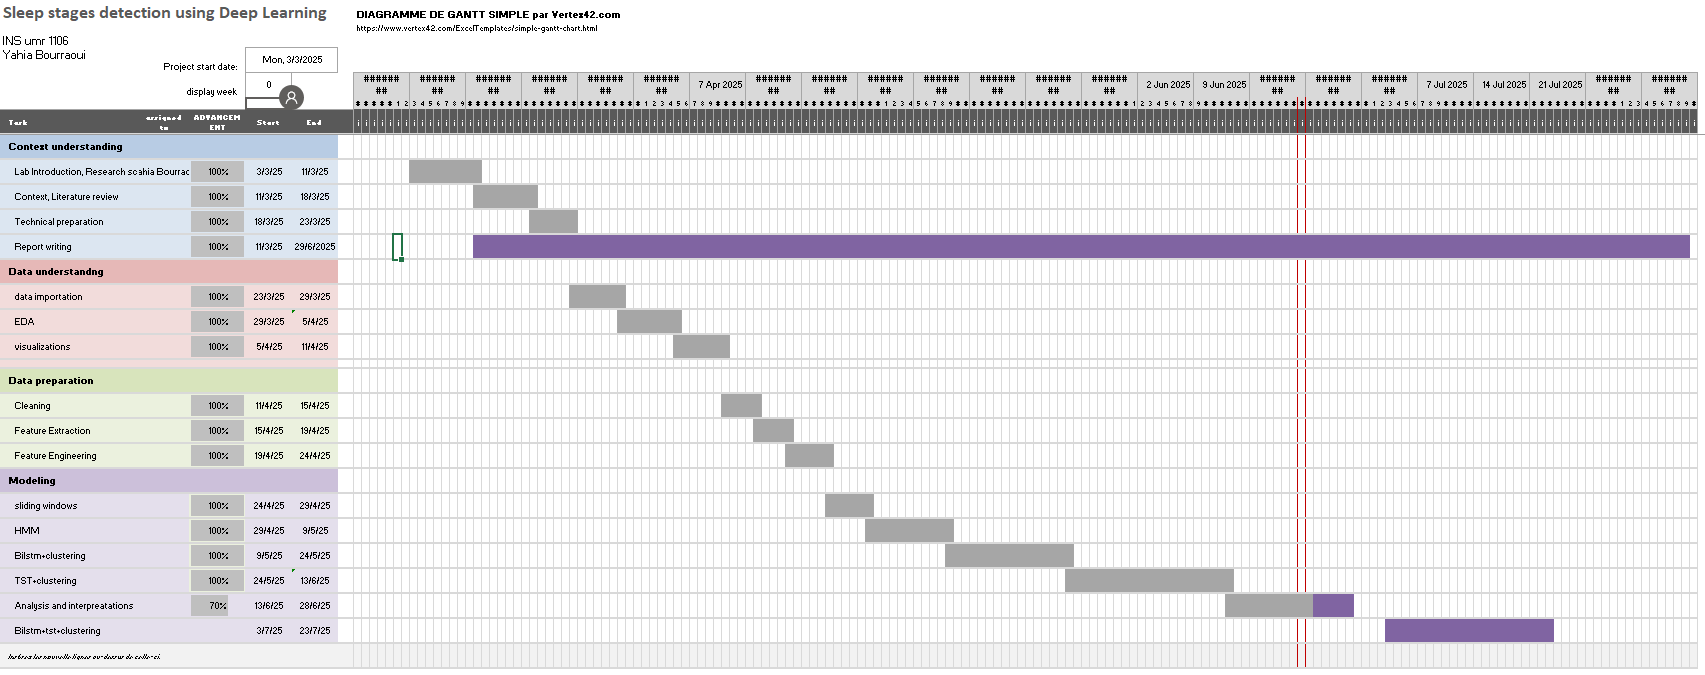
\includegraphics[width=0.95\linewidth]{img/new gantt.png}
    \caption{Project Timeline in Gantt Chart}
    \label{fig:Gantt Diagram}
\end{figure}
\end{landscape}
\clearpage%
}



Having established the project context, organizational structure, and management framework, we now turn our attention to the theoretical foundations and existing literature that inform our approach. The following chapter explores the scientific concepts underlying sleep physiology and neural signal processing, as well as previous research efforts in applying ML techniques to sleep analysis. By building upon this established knowledge base, we position our research within the broader scientific landscape while identifying opportunities for methodological innovation and advancement of the field.

\section{Chapter 2 : Literature Review}
In this chapter, we will define the different notions and concepts that will be exploited, as well
as similar work done on the subject.
\subsection{Neuroscience Notions}

\subsubsection{Sleep Physiology and Architecture}

Sleep represents one of the most fundamental and ubiquitous biological phenomena, constituting approximately one-third of the human lifespan and playing crucial roles in physiological maintenance, cognitive function, and overall health. The scientific understanding of sleep has evolved dramatically over the past century, transitioning from a simple view of sleep as a passive state to recognition of its complex, active, and highly regulated nature \cite{carskadon2017normal}. Modern neuroscience recognizes sleep as a dynamic process involving intricate neural networks, neurotransmitter systems, and oscillatory patterns that orchestrate the transition between consciousness and unconsciousness.

The architecture of sleep exhibits remarkable conservation across mammalian species, suggesting fundamental evolutionary significance while displaying species-specific adaptations that reflect ecological and physiological constraints \cite{siegel2009sleep}. In humans, sleep follows a characteristic architecture composed of Non-Rapid Eye Movement (NREM) and Rapid Eye Movement (REM) stages, each serving distinct physiological functions. NREM sleep encompasses three progressive stages, beginning with light sleep (Stage 1) characterized by the transition from alpha to theta wave dominance, progressing through intermediate sleep (Stage 2) marked by sleep spindles and K-complexes that reflect thalamo-cortical circuit activity, and culminating in deep sleep (Stage 3) dominated by high-amplitude delta waves generated by synchronized cortical neuronal populations.

The neurophysiological mechanisms underlying sleep stage transitions involve complex interactions between multiple brain regions, including the hypothalamic sleep-wake centers, brainstem arousal systems, and thalamo-cortical networks \cite{saper2010sleep}. The suprachiasmatic nucleus serves as the master circadian pacemaker, coordinating sleep timing with environmental light-dark cycles through melatonin secretion and autonomic nervous system regulation. Concurrently, homeostatic sleep pressure, mediated by adenosine accumulation during wakefulness, interacts with circadian influences to determine sleep propensity and architecture.

REM sleep presents a paradoxical state characterized by heightened brain activity resembling wakefulness while maintaining profound muscle atonia and vivid dreaming. This stage emerges through complex interactions between brainstem cholinergic neurons, particularly in the pedunculopontine and laterodorsal tegmental nuclei, which orchestrate the characteristic EEG desynchronization, rapid eye movements, and muscle paralysis. REM sleep serves critical functions in memory consolidation, particularly for procedural and emotional memories, and plays essential roles in brain development and synaptic plasticity.

Comparative analysis reveals that rodent models, particularly rats, exhibit fundamental similarities to human sleep architecture while displaying species-specific characteristics that reflect their ecological niche as nocturnal animals. Rat sleep cycles are considerably shorter, averaging 12-15 minutes compared to human cycles of 90-120 minutes, and rats display polyphasic sleep patterns with multiple brief sleep episodes distributed throughout their active and inactive periods. Despite these temporal differences, the underlying neurochemical and electrophysiological mechanisms show remarkable conservation, making rodent models invaluable for understanding fundamental sleep processes and pathological conditions.

Micro-arousals represent brief interruptions in sleep continuity, typically lasting 3-15 seconds, that may not result in conscious awakening but significantly impact sleep quality and restorative functions. These transient events are characterized by sudden increases in EEG frequency, often accompanied by autonomic nervous system activation including heart rate acceleration and blood pressure elevation. While occasional micro-arousals occur naturally during normal sleep, increased frequency may indicate underlying sleep disorders, respiratory disturbances, or neurological conditions, making their detection and quantification clinically significant for sleep quality assessment \cite{bonnet2007clinical}.

\begin{figure}[H]
    \centering
    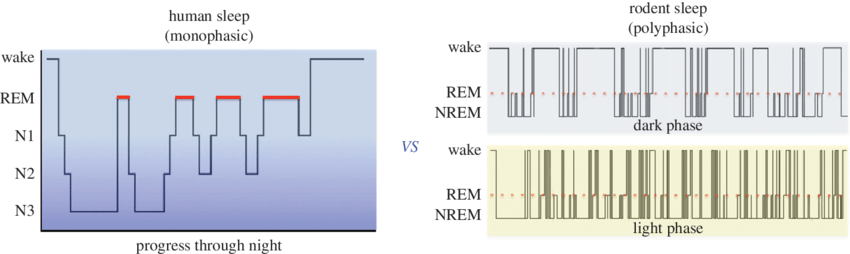
\includegraphics[width=0.8\textwidth]{img/human vs rat sleep.png}
    \caption{Comparison of hypnograms representing typical sleep patterns in humans and rodents. Human sleep is monophasic and normally consists of three to five cycles of the sleep stages throughout the night. Longer bouts of NREMS stage N3 or SWS occur earlier in the night while REMS increases in duration and frequency as the night progresses. Rodent sleep is polyphasic, with wake, NREMS and REMS occurring throughout the light and dark phases. More sleep is acquired in the light phase, while the dark phases consist of consolidated periods of wake. \cite{mong2016sex}}
    \label{fig:sleep_architecture_comparison}
\end{figure}

\begin{enumerate}
    \item \textbf{Human Sleep Architecture}
    
    Humans typically cycle through these stages 4–6 times per night, with the proportion of REM sleep increasing in later cycles.
    
    \item \textbf{Sleep in Rats}
    
    Sleep in rats shares similarities with human sleep but exhibits distinct characteristics due to differences in brain structure and behavior. Like humans, rats experience NREM and REM sleep, but the duration of their sleep cycles is shorter, averaging 12–15 minutes compared to 90–120 minutes in humans.
    
            \textbf{NREM Sleep in Rats:}
    
            Divided into light and deep sleep phases. During NREM sleep, the rat’s EEG displays slow-wave activity similar to that seen in humans.
    
            \textbf{REM Sleep in Rats:}
    
            Characterized by desynchronized EEG patterns, rapid eye movements, and muscle atonia. This stage is shorter in rats but still plays a role in memory consolidation and emotional regulation.
    
    Rats are nocturnal animals and exhibit polyphasic sleep, meaning they sleep in multiple shorter periods distributed throughout the day and night. This contrasts with humans' monophasic sleep pattern.
        
    \item \textbf{Micro-Arousals}
            Micro-arousals are transient events lasting seconds or milliseconds that do not lead to full awakening but interrupt sleep continuity. Despite being hard to detect, they are considered important markers of sleep quality. These events can provide critical insights into sleep disorders and neurological conditions such as epilepsy.
    \end{enumerate}



\subsubsection{Signal Processing Methods for Neural Data}
Signal processing is crucial for analyzing neural data, which often consists of high-dimensional, noisy, and complex signals. To extract meaningful information, several preprocessing steps are applied, including filtering, outlier detection, and data transformation techniques such as standardization and normalization. Below, we expand on these concepts with specific examples relevant to this project.
\begin{enumerate}
    \item \textbf{Filtering}:
    
    \textbf{Bandpass Filters}: Commonly used to isolate specific frequency bands of interest in EEG data, such as:

    \textbf{Delta waves (0.5–4 Hz):} Associated with deep sleep stages.

    \textbf{Theta waves (4–8 Hz):} Linked to light sleep and transitions between sleep stages.

    \textbf{Alpha waves (8–13 Hz):} Observed during relaxed wakefulness.

    \textbf{Beta waves (13–30 Hz):} Present during active cognition and REM sleep.

A bandpass filter can be applied to remove unwanted low-frequency drifts and high-frequency noise. For example, filtering the signal to retain only frequencies between 0.5 and 30 Hz is standard practice in sleep studies and for data containing wake data the filter goes up to 80hz.

    

\item \textbf{Outlier Detection:}

    Neural recordings often contain spikes or irregularities due to technical glitches or unexpected physiological events.
    
    \textbf{Z-Score Analysis}: Outliers can be detected by calculating the Z-score of each data point. Values exceeding a threshold (e.g., ±3 standard deviations) are flagged as potential outliers.
    
    \textbf{Median Absolute Deviation (MAD):} A robust alternative to standard deviation, especially for skewed data.
    
\item \textbf{Standardization and Normalization:}
    Neural data are often recorded on different scales (e.g., voltage, frequency, or power) across channels or sessions. Standardization and normalization ensure that features are comparable and improve the performance of ML models.
        
        \textbf{Standardization:}
        Rescales data to have a mean of 0 and a standard deviation of 1.
        
        Formula:\begin{equation}
        z = \frac{x - \mu}{\sigma}                      \label{eq:standardization}
                    \end{equation}
        
        where:
        \begin{itemize}
            \item $z$ is the standardized value (Z-score)
            \item $x$ is the original data point 
            \item $\mu$ is the mean of the dataset
            \item $\sigma$ is the standard deviation of the dataset
        \end{itemize}


        \item \textbf{Spectrograms}
        A spectrogram is a visual representation of the spectrum of frequencies of a signal as it varies with time. It is generated by segmenting the signal into small time windows and computing the Fourier Transform for each window, producing a time-frequency representation.

        \item \textbf{Spectral Analysis}
        Spectral analysis involves calculating the power spectral density (PSD) of a signal to quantify its energy distribution across different frequency bands. Neural signals, such as EEG, are typically analyzed in terms of their power in specific frequency bands.
        
        \textbf{Frequency Bands:}
        
        \textbf{Delta (0.5–4 Hz):} Dominant during deep sleep (N3 stage).
        
        \textbf{Theta (4–8 Hz):} Prominent in light sleep (N1 and N2 stages) and during transitions between wakefulness and sleep.
        
        \textbf{Alpha (8–13 Hz):} Associated with relaxed wakefulness and sometimes seen during REM sleep.
        
        \textbf{Beta (13–30 Hz):} Linked to active thinking and REM sleep.
        
        \textbf{Gamma (>30 Hz):} Associated with high-level cognitive processes and micro-arousals.

        \textbf{Feature Extraction:}
            
            Calculating the \textbf{relative power} of each band as a feature. For example:
            \begin{equation}
        \text{Relative Power} = \frac{\text{Power in a Band}}{\text{Total Power}}                      \label{eq:relative_power}
                    \end{equation}
        
        where:
        \begin{itemize}
            \item Power in a Band represents the spectral power within a specific frequency range (e.g., delta, theta, alpha)
            \item Total Power is the sum of spectral power across all frequency bands
            \item The result is a normalized measure between 0 and 1 representing the proportion of total power in that frequency band
        \end{itemize}
        
            \textbf{Spectral entropy}, which measures the complexity of the frequency distribution, can help characterize sleep stages and micro-arousals.
\end{enumerate}

\subsubsection{Neurophysiological Signal Measurement and Analysis}

EEG recordings provide valuable insights into neural activity during sleep and wakefulness. The proper understanding of neurophysiological signal properties is essential for developing effective machine learning approaches. These signals exhibit various characteristics:

\begin{itemize}
    \item \textbf{Multi-scale temporal dynamics} - Sleep signals contain information at multiple time scales, from millisecond-level neuronal firing to minute-level sleep stage transitions
    
    \item \textbf{Non-stationary characteristics} - Signal properties change dynamically throughout recording sessions, reflecting state transitions
    
    \item \textbf{Multi-modal integration} - Combining EEG with other physiological measures (EMG, EOG) provides complementary information about sleep states
    
    \item \textbf{Cross-frequency coupling} - Interactions between different frequency bands (e.g., theta-gamma coupling) contain important information about neural state
    
    \item \textbf{Individual variability} - Signal characteristics vary significantly between subjects, requiring robust analytical approaches
\end{itemize}

These neurophysiological properties guide the design of appropriate signal processing and machine learning methodologies for sleep stage analysis and micro-arousal detection.

\subsubsection{EEG Signal Characteristics and Analysis}

EEG signals provide a critical window into neural activity during sleep, capturing oscillatory patterns that distinguish different sleep stages and transient events. These electrophysiological recordings measure voltage fluctuations resulting from ionic current within neurons, reflecting both local processing and distributed network activity across cortical regions.

During wakefulness, EEG patterns typically display low-amplitude, high-frequency activity, particularly in the beta (13-30 Hz) range, reflecting active cognitive processing and desynchronized neural activity. As an individual transitions into light sleep (N1 stage), alpha rhythms (8-13 Hz) diminish while theta oscillations (4-7 Hz) become more prominent, marking the initial disengagement from conscious awareness.

Intermediate sleep (N2 stage) introduces characteristic waveforms including sleep spindles and K-complexes. Sleep spindles are short bursts of oscillatory activity in the sigma band (11-16 Hz) that reflect thalamocortical circuit activation and play critical roles in memory consolidation and sensory gating during sleep. K-complexes, characterized by distinctive high-amplitude biphasic waves, represent synchronized neuronal responses that may serve protective functions by suppressing arousal to non-threatening stimuli while enabling awakening to potentially significant disturbances.

Deep sleep (N3 stage) exhibits high-amplitude delta waves (0.5-4 Hz), reflecting widespread synchronization of cortical neurons alternating between depolarized up-states and hyperpolarized down-states. This slow-wave activity correlates with synaptic homeostasis processes essential for cognitive function and reflects the highest threshold for arousal.

REM sleep presents a paradoxical EEG pattern, with desynchronized, low-amplitude, mixed-frequency activity resembling wakefulness despite profound behavioral sleep. This stage is characterized by sawtooth waves, transient sharp waves in the theta range that often precede rapid eye movements, and the suppression of higher-voltage, lower-frequency components seen in NREM sleep.

Micro-arousals manifest as abrupt frequency shifts in the EEG, typically from delta or theta rhythms toward alpha or beta activity, lasting between 3-15 seconds without producing full behavioral awakening. These events often display distinctive spectral characteristics, including rapid power increases in higher frequency bands (>16 Hz) and concurrent alterations in autonomic measures including heart rate and respiratory patterns.

Quantitative EEG analysis techniques employed in this research include time-domain statistics (amplitude distributions, zero-crossing rates), frequency-domain measures (spectral power across traditional frequency bands), time-frequency analyses (wavelet transforms, spectrograms), and non-linear methods (entropy calculations, phase synchronization indices). These complementary approaches capture different aspects of the complex, non-stationary neural dynamics underlying sleep architecture and micro-arousal phenomena.

Given the high-dimensional, sequential nature of EEG data and the complex temporal patterns within frequency bands, machine learning approaches are required to automate pattern recognition and classification tasks.

\subsection{ML for Sequential Data}  %for sequential data
ML (ML) provides a powerful set of tools for analyzing complex data in neuroscience, including time series data from sleep studies. This section explores relevant ML approaches, focusing on unsupervised learning, recurrent neural networks, clustering algorithms, and transformer-based models, including self-supervised learning techniques.

\subsubsection{Unsupervised Learning}
    
    Unsupervised learning involves discovering hidden patterns or structures in unlabeled data. In the context of neuroscience, it is often used for clustering, dimensionality reduction, and identifying latent variables in neural activity or biometric signals.
    \begin{itemize}
        \item \textbf{Clustering Algorithms}
        
            \textbf{K-Means}: A popular centroid-based clustering algorithm that partitions data into 
            
            \textbf{k clusters} by minimizing the within-cluster variance. For sleep stage analysis, K-Means can help group similar signal patterns.
            
            \textbf{HDBSCAN }(Hierarchical Density-Based Spatial Clustering of Applications with Noise): An advanced clustering algorithm capable of handling data with varying densities and noise. It is suitable for analyzing complex, non-linear structures in sleep-related signals.
            
            \textbf{Spectral Clustering}: Utilizes graph-based representations of data for clustering. It is useful when the data structure is non-convex, making it ideal for separating overlapping sleep stage signals.
        \item \textbf{Dimensionality Reduction:}

            Techniques such as \textbf{Principal Component Analysis (PCA), UMAP and t-SNE (t-distributed Stochastic Neighbor Embedding)} are often used to visualize high-dimensional data and reduce noise before clustering.

    \end{itemize}

\subsubsection{Bidirectional Long Short-Term Memory (BiLSTM)}

Bidirectional Long Short-Term Memory (BiLSTM) networks are a variant of the LSTM architecture designed to capture dependencies in both forward and backward directions of sequential data. This is particularly advantageous for tasks requiring contextual understanding from past and future information.

\begin{itemize}
    \item \textbf{Architecture:} BiLSTMs consist of two LSTM networks running in parallel—one processes the sequence from start to end, and the other processes it from end to start. The hidden states from both directions are concatenated to provide a comprehensive representation of the sequence.
    \item \textbf{Applications:} BiLSTMs have been applied in numerous domains such as speech recognition, text analysis, and EEG signal classification. For example, they have been used to classify sleep stages by analyzing EEG sequences, capturing both preceding and succeeding signal patterns.
    \item \textbf{Strengths:} The ability to learn bidirectional dependencies makes BiLSTMs ideal for tasks where the context around a data point significantly influences the outcome.
\end{itemize}

\subsubsection{Time Series Transformers}

Transformers, initially introduced for natural language processing, have been adapted for time-series data analysis due to their ability to model long-range dependencies and handle high-dimensional data. The Time Series Transformer is specifically tailored for sequential data.

\begin{itemize}
    \item \textbf{Architecture:} The core of a Transformer is its attention mechanism, which assigns varying importance to different parts of the input sequence. This allows the model to focus on relevant features without being constrained by sequential processing.
    \item \textbf{Applications:} Time Series Transformers have shown promise in tasks such as forecasting, anomaly detection, and clustering. In EEG analysis, they enable the discovery of micro-arousals and subtle patterns that may be missed by traditional models.
    \item \textbf{Strengths:} 
    \begin{itemize}
        \item \textbf{Scalability:} Handles large datasets efficiently by parallelizing computations.
        \item \textbf{Flexibility:} Adaptable to various input types, including multivariate and multi-channel signals.
        \item \textbf{Comprehensive Context Modeling:} Captures complex dependencies across entire sequences.
    \end{itemize}
\end{itemize}

\subsection{Review of Existing Literature}

The following comprehensive literature review examines key methodological approaches that directly inform and support the research objectives of this work. Each selected paper contributes essential theoretical foundations, methodological insights, or empirical evidence that advances our understanding of automated sleep analysis and micro-arousal detection using ML techniques.

\subsubsection{Foundational Approaches to Time Series Analysis and Data Streaming}

Real-time Data Stream Clustering Over Sliding Windows \cite{aggarwal2003framework} represents a seminal contribution to the field of continuous physiological signal analysis. This work directly addresses the computational challenges encountered when processing the extensive temporal datasets characteristic of long-term sleep monitoring studies, such as our 30-day rodent recordings and multi-night human polysomnographic data.

The sliding window paradigm proposed by \citeauthor{aggarwal2003framework} provides the theoretical foundation for our time series segmentation strategy, enabling efficient processing of continuous EEG streams while preserving temporal dependencies essential for micro-arousal detection. Their framework's ability to maintain fixed computational complexity regardless of stream length directly supports our research objective of developing scalable algorithms suitable for clinical deployment. The concept drift adaptation mechanisms described in their work prove particularly relevant for handling the natural variability in sleep patterns across different subjects and recording conditions encountered in our datasets.

Building upon this foundation, the comprehensive survey by \citeauthor{gama2014survey} \cite{gama2014survey} provides critical insights into adaptive learning strategies essential for non-stationary biological signals. Their taxonomy of concept drift types—sudden, gradual, incremental, and recurring—maps directly onto the challenges observed in sleep architecture analysis, where sleep patterns evolve throughout the night and across multiple recording sessions. This theoretical framework informs our model selection criteria and evaluation strategies, particularly for assessing model robustness across different patient populations and recording environments.

The data stream models proposed by \citeauthor{babcock2002models} \cite{babcock2002models} offer practical implementation strategies for managing memory constraints while preserving analytical precision. Their sliding window algorithms directly inform our preprocessing pipeline design, particularly the selection of optimal window sizes that balance temporal resolution with computational efficiency. For our micro-arousal detection objectives, their findings regarding window size selection (30 seconds to several minutes) align with the temporal characteristics of sleep-related transient events identified in clinical literature.

These foundational works collectively establish the theoretical and practical framework necessary for implementing robust, scalable algorithms capable of processing continuous physiological signals in real-time clinical environments. Their contributions directly address the computational challenges identified in our research objectives while providing validated approaches for handling the temporal complexity inherent in sleep analysis.

\subsubsection{Machine Learning Models and Neural Architectures for Sleep Classification}

Multi-Domain Feature Extraction and Ensemble Learning \cite{Wang2025} represents a significant advancement in interpretable ML for sleep analysis, directly addressing the clinical requirement for transparent, explainable automated systems. The XGBoost-based approach demonstrated by \citeauthor{Wang2025} achieves state-of-the-art classification performance while maintaining the interpretability essential for clinical acceptance and regulatory approval.

Their comprehensive feature extraction strategy, encompassing temporal, spectral, and nonlinear signal characteristics, provides the methodological foundation for our feature engineering pipeline. The demonstrated superiority of multi-domain approaches (85.3\% accuracy) over single-domain methods (76.8\% accuracy) directly supports our decision to implement comprehensive feature extraction spanning multiple signal analysis domains. Their feature importance rankings reveal that spectral power features in delta (0.5-4 Hz) and sigma (11-15 Hz) bands contribute most significantly to classification accuracy, providing guidance for our own feature selection strategies.

Particularly relevant to our research objectives, their interpretability analysis demonstrates how ensemble methods can provide clinically meaningful insights into sleep physiology while maintaining high classification accuracy. The feature importance visualizations they present offer templates for developing clinical decision support systems that enable practitioners to understand and validate automated recommendations. This transparency addresses the critical barrier to clinical adoption of ML systems in sleep medicine.

The robustness analysis performed across diverse patient populations, including different age groups and pathological conditions, provides validation strategies applicable to our own evaluation framework. Their cross-dataset validation, demonstrating consistent performance across Sleep-EDF, MASS, and SHHS databases, establishes benchmarks for evaluating the generalizability of our own algorithms across different recording environments and patient populations.

DL and Neural Architecture Innovation \cite{supratak2017deepsleepnet} has revolutionized automated sleep staging through the introduction of end-to-end learning approaches that eliminate the need for manual feature engineering. The DeepSleepNet architecture demonstrates how convolutional and recurrent neural networks can be effectively combined for physiological signal analysis, achieving performance levels (82.0\% overall accuracy) that approach inter-scorer agreement rates among human experts.

The hierarchical feature learning approach demonstrated by \citeauthor{supratak2017deepsleepnet} directly informs our DL implementation strategy, particularly the combination of convolutional layers for local feature extraction with recurrent layers for temporal dependency modeling. Their two-stage training procedure—pretraining on representation learning followed by fine-tuning for classification—provides methodological guidance for optimizing DL models on limited annotated sleep data.

Critical to our research objectives, their work demonstrates the feasibility of processing raw single-channel EEG signals without requiring extensive preprocessing or domain expertise for feature engineering. This capability aligns with our goal of developing automated systems suitable for deployment in diverse clinical environments where specialized signal processing expertise may not be available.

The sequence-to-sequence modeling capabilities they demonstrate prove particularly relevant for our micro-arousal detection objectives, as these events often exhibit temporal patterns spanning multiple epochs. Their ability to model dependencies across 20-second epochs provides the temporal context necessary for detecting subtle patterns characteristic of micro-arousals and sleep stage transitions.

Self-Supervised Learning for Physiological Signal Analysis \cite{banville2021uncovering} addresses the fundamental challenge of limited annotated datasets in neuroscience research while demonstrating novel approaches to discovering hidden patterns in physiological signals. This work directly supports our unsupervised learning objectives by providing validated methodologies for extracting meaningful representations from unlabeled EEG data. The contrastive learning framework presented by \citeauthor{banville2021uncovering} offers powerful tools for learning discriminative representations that capture clinically relevant patterns without requiring extensive manual annotations. Their approach, achieving 79.3\% classification accuracy using only 1\% of labeled data, demonstrates the potential for discovering novel sleep substates and micro-arousal patterns not captured by traditional scoring criteria.

Particularly significant for our work, their self-supervised pretraining approach enables effective utilization of the extensive unlabeled portions of our datasets, including the continuous 30-day rodent recordings where manual annotation would be prohibitively expensive. The representations learned through their contrastive approach capture temporal dependencies essential for modeling sleep architecture while remaining robust to inter-subject variability and recording artifacts.

Transformer Architectures for Sleep Analysis \cite{phan2019sleeptransformer} represents the state-of-the-art in sequence modeling for physiological signals, demonstrating how attention mechanisms can capture complex temporal dependencies spanning extended time periods. The SeqSleepNet architecture achieves superior performance (87.1\% overall accuracy) compared to traditional RNN-based approaches while providing interpretable attention patterns that highlight clinically relevant signal segments. The hierarchical attention mechanism they implement—combining epoch-level and sequence-level attention—provides methodological guidance for our Transformer implementation strategy. Their demonstration that longer sequence contexts (up to 25 epochs) improve classification accuracy directly supports our decision to implement sequence-based training strategies that preserve temporal continuity across extended recording periods.



Critical to our micro-arousal detection objectives, their attention visualizations reveal how Transformer models automatically identify transient events and stage transition periods, often focusing attention on the same signal segments that human experts mark as clinically significant. This interpretability enhances clinical acceptance while providing validation that automated systems are learning physiologically meaningful patterns.

\subsubsection{Dynamic Mode Decomposition and Physics-Informed Methods}

DMD for Electrocorticographic Signal Decoding \cite{Yanagisawa2024} provides direct empirical support for applying Dynamic Mode Decomposition techniques to neurophysiological signal analysis. This recent work demonstrates that DMD-based feature extraction significantly outperforms conventional spectral analysis methods for decoding neural signals, achieving 75.3\% accuracy compared to 68.1\% for power-based features in motor imagery tasks.

The spatial-DMD (sDM) features developed by \citeauthor{Yanagisawa2024} offer computational advantages particularly relevant to our real-time processing objectives, reducing computational requirements by approximately 40\% compared to kernel-based methods while maintaining superior classification performance. Their demonstration that sDM features capture spatiotemporal coherence patterns provides theoretical justification for our application of DMD techniques to sleep analysis, where similar spatiotemporal patterns characterize sleep stages and micro-arousals.

Most significantly for our research objectives, their work establishes the biological interpretability of DMD-based features, demonstrating clear correlations between sDM components and neurophysiologically relevant activation patterns. This interpretability addresses the critical clinical requirement for transparent, explainable automated systems while providing confidence that DMD-based approaches capture meaningful physiological phenomena rather than statistical artifacts.

The computational efficiency demonstrated in their work—enabling near-real-time processing of high-density neural signals—directly supports our objective of developing clinically deployable algorithms. Their implementation achieves processing speeds suitable for online applications while maintaining the temporal resolution necessary for detecting rapid transient events like micro-arousals.

Critically, DMD-based approaches provide physics-informed methods that combine the interpretability requirements for clinical deployment with the performance advantages of advanced mathematical frameworks. The demonstrated biological relevance and computational efficiency of these methods directly support our objective of developing practical, deployable solutions for automated sleep analysis. This research direction complements other methodological approaches in our study, including streaming data processing, probabilistic modeling, and deep learning techniques.

The integration of these diverse methodological approaches provides a comprehensive analytical framework necessary for addressing the complex challenges inherent in automated micro-arousal detection and sleep analysis. DMD and physics-informed methods offer valuable contributions to this framework, providing interpretable features with strong biological relevance while addressing limitations of purely statistical approaches. This integration advances both scientific understanding and practical applications in sleep medicine, representing a significant contribution to the field of computational neuroscience.



\begin{table}[H]
\centering
\caption{Summary of Key Literature and Methodological Approaches}
\begin{tabular}{|p{2.5cm}|p{3cm}|p{3cm}|p{5cm}|}
\hline
\textbf{Approach} & \textbf{Key References} & \textbf{Main Contributions} & \textbf{Relevance to Current Study} \\
\hline
Time Series Analysis & Aggarwal et al. (2003), Gama et al. (2014) & Sliding window paradigm, adaptive learning strategies for non-stationary signals & Foundation for temporal segmentation and computational efficiency in long-term recordings \\
\hline
Sleep Classification Models & Pan et al. (2012), Wang (2025) & Dynamic HMMs for sequential data, multi-domain feature extraction strategies & Probabilistic modeling framework for sleep stage transitions and micro-arousal detection \\
\hline
Neural Architectures & Supratak et al. (2017), Phan et al. (2019), Banville et al. (2021) & End-to-end learning, self-supervised approaches, transformer architectures & Novel pattern discovery in unlabeled data, capturing long-range temporal dependencies \\
\hline
Physics-Informed Methods & Yanagisawa (2024), Brunton et al. (2016) & DMD for neurophysiological signals, spatiotemporal coherence patterns & Biologically interpretable feature extraction while maintaining computational efficiency \\
\hline
\end{tabular}
\label{tab:literature_summary}
\end{table}

This summary provides a consolidated overview of the key methodological approaches informing our research. By integrating these complementary techniques, we develop a robust analytical framework capable of addressing the complex challenges inherent in automated sleep analysis while maintaining biological interpretability essential for clinical applications.

Having examined the theoretical foundations and reviewed relevant literature, we now proceed to a detailed discussion of our data understanding and processing methodology. The following section explores our approach to analyzing the complex physiological signals that form the basis of our investigation, applying many of the techniques identified in our literature review while addressing the unique challenges presented by our specific datasets.


\section{Chapter 3 : Data Understanding and Processing}

The foundation of any successful ML endeavor lies in comprehensive data understanding and meticulous processing. Following the CRISP-DM methodology, this chapter addresses the critical second and third phases: data understanding and data processing. Our investigation focuses on exploring and analyzing sequential physiological data through multiple analytical lenses, employing diverse methodological approaches to determine optimal strategies for uncovering hidden patterns within complex biological signals.

In the context of sleep research and neurophysiological signal analysis, the objective transcends traditional accuracy-driven ML paradigms. Rather than conforming to predefined ground truths, our unsupervised learning approach aims to discover latent structures and novel insights that may reveal previously unrecognized phenomena within sleep architecture and neural dynamics. This exploratory philosophy guides our analytical framework, emphasizing pattern discovery over validation of existing knowledge.

The chapter begins with comprehensive dataset characterization, examining the unique properties and inherent challenges of both rodent and human physiological recordings. We then progress through sophisticated exploratory analysis techniques that reveal the complex temporal dependencies underlying sleep-related neural activity. Our investigation culminates in the justification and implementation of advanced mathematical frameworks, particularly Dynamic Mode Decomposition (DMD) and its extensions, which provide powerful tools for extracting meaningful features from high-dimensional physiological signals while preserving their dynamic characteristics.

\subsection{Data Description and Exploratory Analysis}

Understanding the fundamental characteristics of our datasets is paramount for developing appropriate analytical strategies. Our investigation encompasses two distinct but complementary datasets: continuous long-term rodent recordings and comprehensive human polysomnographic studies. Each dataset presents unique opportunities and challenges that shape our methodological approach.

\subsubsection{Rat Dataset: Long-term Continuous Monitoring}

The rodent dataset represents an unprecedented opportunity to study natural sleep-wake cycles over extended periods without the environmental confounds typically associated with human studies. This dataset comprises continuous physiological recordings spanning 30 consecutive days, providing an exceptional window into the natural rhythms and long-term dynamics of mammalian sleep regulation.

The electroencephalographic component consists of single-channel recordings from the frontal cortical region, captured at a robust sampling frequency of 512 Hz. This high temporal resolution ensures preservation of fine-grained oscillatory patterns across the entire frequency spectrum relevant to sleep analysis, from slow-wave delta rhythms to rapid gamma-band activity. The sampling rate exceeds the Nyquist criterion for all physiologically relevant frequencies, enabling accurate reconstruction of neural dynamics without aliasing artifacts that could compromise subsequent analyses.

Complementing the neural recordings, continuous activity monitoring was conducted using accelerometry-based sensors sampling at 16 Hz. While this lower sampling frequency might initially appear limiting, it proves optimal for capturing gross motor patterns while minimizing data storage requirements. The activity signal provides crucial contextual information for distinguishing active wakefulness from quiet rest states, thereby enhancing the interpretability of concurrent neural activity patterns.

The controlled laboratory environment ensured minimal external interference throughout the recording period, maintaining consistent environmental conditions that facilitate the study of intrinsic circadian and ultradian rhythms. This experimental design enables investigation of natural sleep architecture evolution over multiple weeks, revealing long-term adaptation patterns and potential cyclical variations that might be missed in shorter recording sessions.

The extended 30-day duration offers unique advantages for unsupervised learning approaches, providing sufficient data for discovering rare events, long-term trends, and complex pattern interactions that require extensive temporal context. However, this temporal richness also introduces challenges related to signal stationarity, as physiological parameters may drift over extended periods due to factors such as adaptation, aging, or environmental changes. The single-channel nature of the EEG recording, while limiting spatial resolution compared to multi-electrode arrays, provides sufficient information for fundamental sleep stage discrimination and micro-arousal detection while maintaining data manageable complexity.

\subsubsection{Human Dataset: Comprehensive Polysomnographic Analysis}

Our human dataset draws from the prestigious Sleep-EDF Database Expanded, an open-access repository maintained by PhysioNet that has become a cornerstone resource for sleep research worldwide. This comprehensive collection contains 197 whole-night polysomnographic recordings, each meticulously annotated according to established clinical standards, providing an invaluable resource for both supervised and unsupervised learning approaches.

The dataset's foundation rests on the Sleep Cassette study, conducted between 1987 and 1991, which examined age-related sleep changes across a diverse cohort of healthy Caucasian adults spanning ages 25 to 101 years. This demographic breadth provides exceptional opportunities for investigating age-related changes in sleep architecture while maintaining consistency in recording methodologies and annotation standards. The exclusion of individuals taking sleep-related medications ensures that observed patterns reflect natural physiological processes rather than pharmacological influences.

Each recording encompasses multiple physiological modalities essential for comprehensive sleep analysis. The electroencephalographic signals are acquired from two standard locations—Fpz-Cz and Pz-Oz—according to the international 10-20 electrode placement system. These electrode positions provide complementary perspectives on cortical activity, with Fpz-Cz capturing frontal-central dynamics often associated with slow-wave activity, while Pz-Oz reflects parietal-occipital patterns characteristic of different sleep stages. The 100 Hz sampling frequency, while lower than our rodent recordings, meets clinical standards and provides adequate resolution for standard sleep scoring and micro-arousal detection.

Electrooculographic recordings from horizontal electrode placements capture the characteristic rapid eye movements that define REM sleep, while submental electromyographic signals reflect muscle tone changes that distinguish between sleep stages and movement artifacts. These signals undergo specialized preprocessing, with EMG signals being high-pass filtered, rectified, and envelope-detected before 1 Hz sampling, providing a robust indicator of muscle activity while minimizing storage requirements.

Additional physiological parameters, including oro-nasal airflow and rectal body temperature, expand the analytical possibilities beyond traditional sleep staging. The airflow measurements enable investigation of respiratory-related events and their relationships with sleep architecture, while temperature monitoring provides insights into circadian rhythm influences on sleep patterns.

The recording methodology employed portable cassette-tape systems that allowed subjects to maintain their normal home environments and daily routines. This naturalistic approach enhances ecological validity compared to laboratory-based studies, potentially revealing sleep patterns that more accurately reflect real-world conditions. Each subject contributed approximately 20 hours of continuous recording spanning two consecutive day-night cycles, providing sufficient data for comprehensive analysis while minimizing subject burden.

The manual annotation process, conducted by trained technicians following the Rechtschaffen and Kales manual, provides gold-standard sleep stage classifications including Wake (W), REM (R), and Non-REM stages 1-4, along with movement time (M) and unscored epochs (?). These annotations serve as valuable benchmarks for evaluating unsupervised approaches while acknowledging that our exploratory analyses may reveal patterns not captured by traditional staging criteria.

\begin{figure}
    \centering
    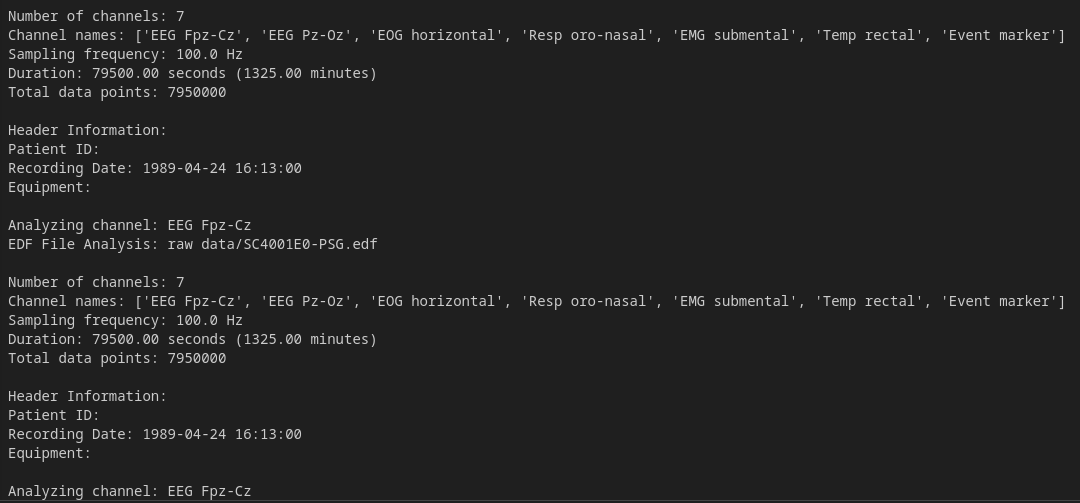
\includegraphics[width=0.95\textwidth]{img/data description.png}
    \caption{Human data file description showing the comprehensive polysomnographic recording structure and signal characteristics from the Sleep-EDF Database Expanded.}
    \label{fig:human_data_description}
\end{figure}






\subsubsection{Exploratory Data Analysis: Multi-Domain Signal Characterization}

Comprehensive exploratory analysis forms the cornerstone of understanding complex physiological signals, requiring sophisticated approaches that capture both temporal and spectral characteristics while revealing underlying dynamic structures. Our analytical framework encompasses multiple complementary domains, each providing unique insights into the intricate patterns embedded within sleep-related neural activity.

\textbf{Amplitude Envelope Analysis and Temporal Dynamics}

Amplitude envelope analysis serves as a fundamental tool for understanding signal energy distribution and temporal variability patterns within physiological recordings. This technique proves particularly valuable for identifying state transitions and detecting anomalous events that manifest as amplitude modulations across different temporal scales. In sleep research, envelope analysis reveals critical information about arousal patterns, sleep depth variations, and the temporal structure of different sleep stages.

The methodology involves extracting the instantaneous amplitude envelope using the Hilbert transform, which provides a smooth representation of signal magnitude variations while preserving temporal resolution. This approach effectively captures both rapid amplitude fluctuations associated with micro-arousals and slower modulations reflecting deeper sleep stage transitions. For our rodent dataset, envelope analysis successfully highlights the dramatic amplitude differences between active wakefulness and quiet sleep states, while in human recordings, it reveals the subtle amplitude variations characteristic of different sleep stages and the pronounced increases associated with movement artifacts and awakening episodes.

\begin{figure}[h]
  \centering
  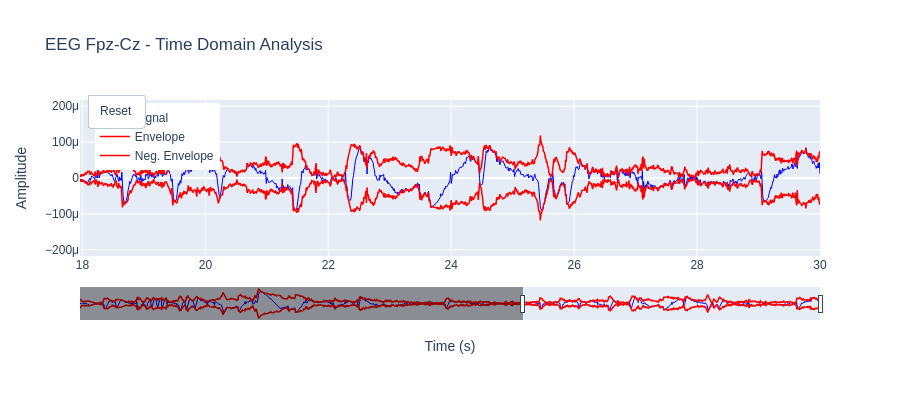
\includegraphics[width=0.9\linewidth]{img/eeg fpz cz time domain analysis}
  \caption{Time domain analysis of human EEG data from Fpz-Cz electrode placement, demonstrating amplitude envelope characteristics and temporal patterns over approximately 12 seconds of recording.}
  \label{fig:eeg_fpz_cz_time_domain}
\end{figure}

\begin{figure}[h]
  \centering
  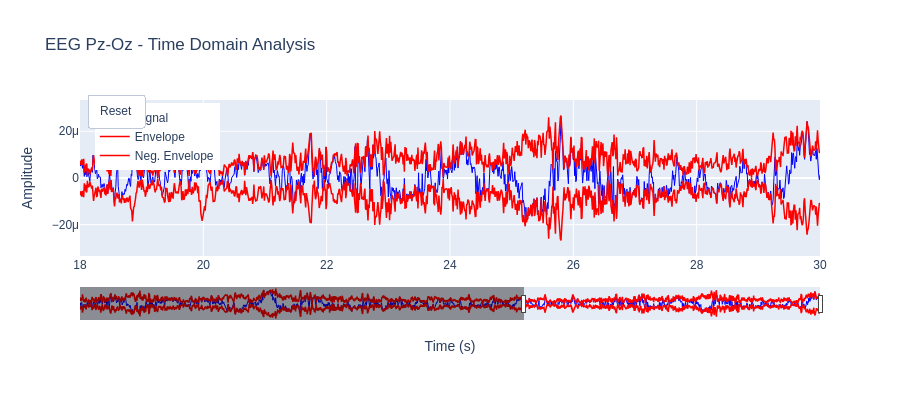
\includegraphics[width=0.9\linewidth]{img/eeg pz oz time domain analysis}
  \caption{Time domain analysis of human EEG data from Pz-Oz electrode placement, revealing distinct amplitude patterns and oscillatory characteristics compared to the frontal-central recording.}
  \label{fig:eeg_pz_oz_time_domain}
\end{figure}

\begin{figure}[H]
  \centering
  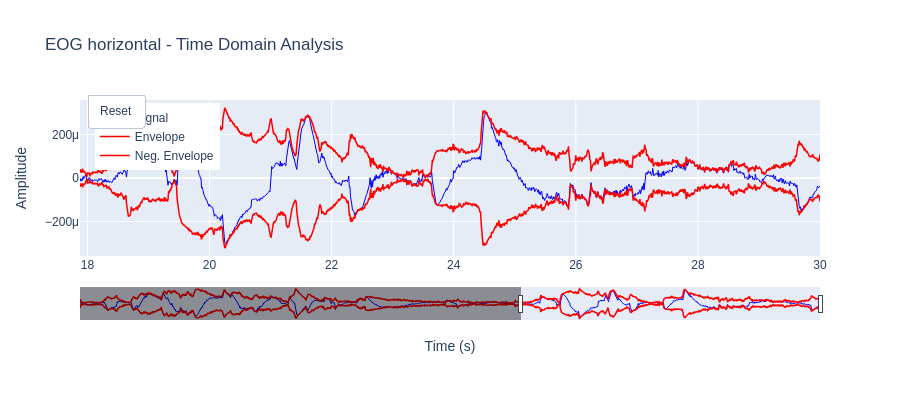
\includegraphics[width=0.9\linewidth]{img/eog horizontal time domain analysis}
  \caption{Time domain analysis of horizontal electrooculographic (EOG) signals, capturing characteristic eye movement patterns and their temporal dynamics during sleep-wake transitions.}
  \label{fig:eog_horizontal_time_domain}
\end{figure}

The comparative analysis of signals from different electrode locations reveals fascinating insights into the spatial distribution of neural activity patterns. Despite originating from the same neural system and representing concurrent time windows, the EEG signals from Fpz-Cz and Pz-Oz electrode positions exhibit markedly different amplitude characteristics and temporal dynamics. These differences reflect the spatial heterogeneity of cortical activity and highlight the importance of multi-channel approaches for comprehensive sleep analysis.

The envelope analysis proves instrumental in highlighting regional variations that might otherwise be obscured in raw time-series data. By examining the envelope signal, which encapsulates the waveform boundaries, we effectively account for the signal's inherent variability while maintaining sensitivity to amplitude-based phenomena such as sleep spindles, K-complexes, and arousal-related amplitude increases. This technique provides exceptional clarity in visualizing amplitude dynamics, enabling identification of temporal patterns and variations that remain hidden in conventional time-domain visualization approaches.

\textbf{Frequency-Domain Characterization and Spectral Analysis}

Frequency-domain analysis represents an indispensable component of physiological signal investigation, revealing the spectral composition and rhythmic structure underlying complex neural dynamics. Through sophisticated spectral decomposition techniques, including Fourier transforms and advanced time-frequency methods, we uncover the fundamental oscillatory patterns that characterize different sleep stages and physiological states.

The methodology employs power spectral density estimation to quantify frequency-specific energy distributions, with particular attention to clinically relevant frequency bands including delta (0.5-4 Hz), theta (4-8 Hz), alpha (8-13 Hz), sigma (11-15 Hz), and beta (13-30 Hz) ranges. Each frequency band carries distinct physiological significance, with delta rhythms indicating deep sleep, theta activity associated with REM sleep and drowsiness, alpha rhythms reflecting relaxed wakefulness, sigma frequencies encompassing sleep spindles, and beta activity indicating active wakefulness or arousal states.

\begin{figure}[h]
  \centering
  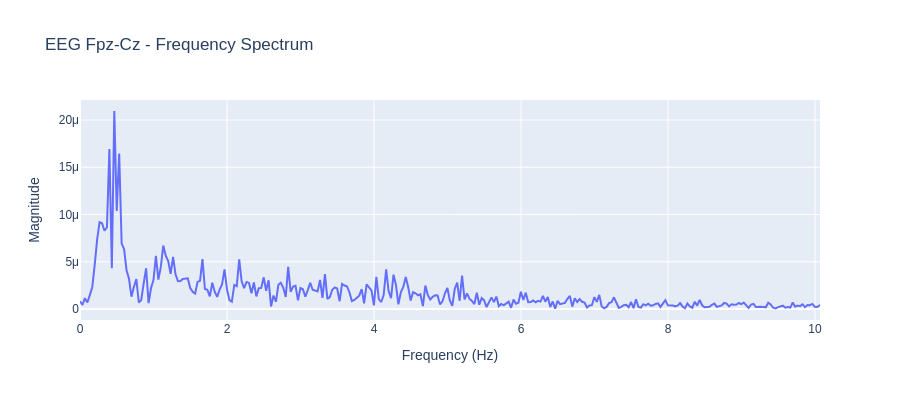
\includegraphics[width=0.9\linewidth]{img/frequency spectrum eeg Fpz-Cz}
  \caption{Frequency spectrum analysis of EEG signal from Fpz-Cz electrode placement, limited to 10Hz to emphasize low-frequency components critical for sleep stage characterization.}
  \label{fig:freq_spectrum_fpz_cz}
\end{figure}

\begin{figure}[h]
  \centering
  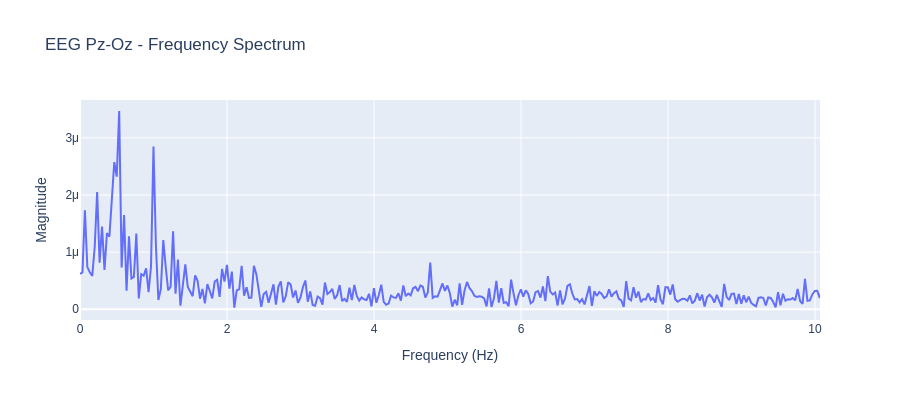
\includegraphics[width=0.9\linewidth]{img/frequency spectrum EEG Pz-Oz}
  \caption{Frequency spectrum analysis of EEG signal from Pz-Oz electrode placement, revealing distinct spectral characteristics compared to frontal-central recordings.}
  \label{fig:freq_spectrum_pz_oz}
\end{figure}

\begin{figure}[H]
  \centering
  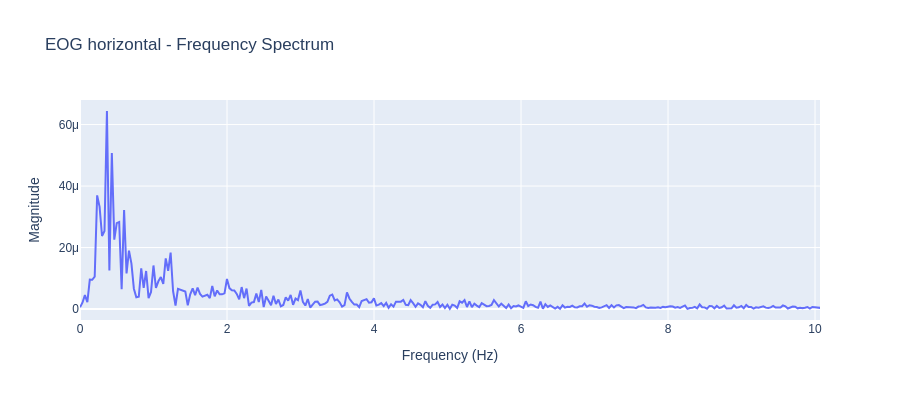
\includegraphics[width=0.9\linewidth]{img/frequency spectrum EOG Horizontal}
  \caption{Frequency spectrum analysis of horizontal EOG signal, demonstrating the characteristic low-frequency components associated with eye movement artifacts and sleep-related ocular dynamics.}
  \label{fig:freq_spectrum_eog_horizontal}
\end{figure}

Our spectral analysis reveals compelling insights into the frequency domain characteristics of different physiological signals. The decision to limit frequency analysis to 10 Hz reflects practical considerations based on the observation that higher frequency components exhibit diminishing amplitude and contribute minimally to sleep-related pattern recognition. This frequency limitation aligns with clinical sleep scoring practices while reducing computational complexity and noise interference from high-frequency artifacts.

The comparative spectral analysis across different signal modalities reveals distinct frequency signatures that reflect their physiological origins. EEG signals exhibit the characteristic frequency-dependent power distributions associated with cortical activity, with prominent peaks in delta and alpha ranges depending on the sleep-wake state. EOG signals demonstrate predominantly low-frequency characteristics reflecting the mechanical properties of eye movements, while EMG signals show broader frequency distributions related to muscle activity patterns.

Frequency domain visualization provides superior precision and detail compared to time-domain envelope analysis, enabling quantitative assessment of spectral power distributions and facilitating objective comparison across different recording conditions and subjects. This enhanced precision proves crucial for detecting subtle spectral changes associated with micro-arousals, sleep stage transitions, and pathological conditions that might be missed through purely temporal analysis approaches.

\textbf{Advanced Visualization Techniques and Time-Frequency Analysis}

Modern sleep research demands sophisticated visualization approaches that can simultaneously capture temporal evolution and spectral characteristics of complex physiological signals. Advanced visualization techniques, including spectrograms, time-frequency representations, and interactive exploration tools, provide comprehensive insights into the dynamic spectral evolution that characterizes sleep architecture and associated phenomena.

\begin{figure}[H]
  \centering
  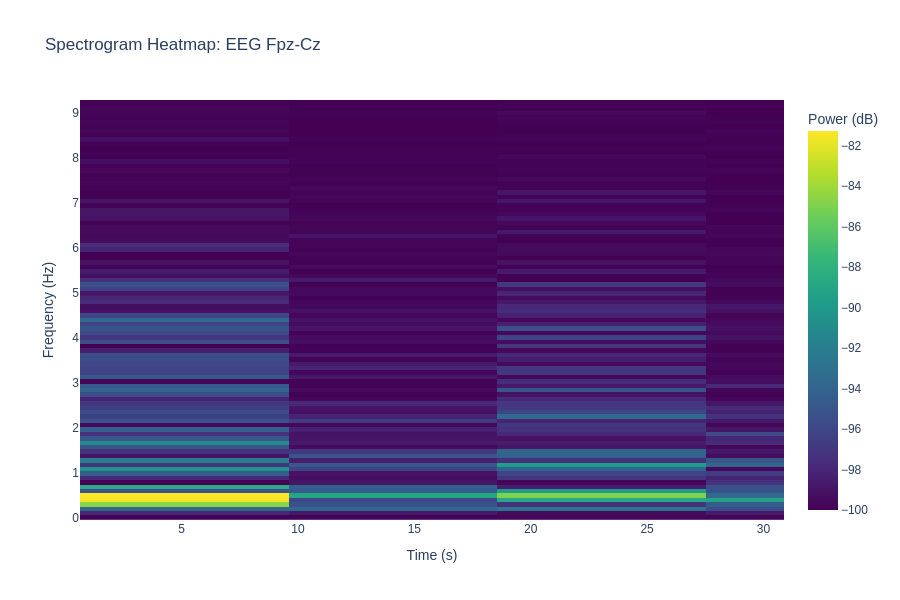
\includegraphics[width=0.9\linewidth]{img/spectrogram heatmap}
  \caption{Spectrogram heatmap visualization demonstrating time-frequency analysis capabilities for revealing dynamic spectral evolution patterns within physiological signals.}
  \label{fig:spectrogram_heatmap}
\end{figure}

The implementation of multitaper spectrogram analysis provides exceptional time-frequency resolution while minimizing spectral leakage artifacts that can compromise traditional Fourier-based approaches. Although applied to relatively large time windows for demonstration purposes rather than detailed micro-analysis, the heat map visualization effectively highlights the presence and temporal evolution of distinct frequency bands, particularly the clinically significant delta and theta oscillations.

The spectrogram analysis proves particularly valuable during periods of physiological transition, where traditional steady-state analysis approaches may fail to capture the dynamic nature of neural activity. In our demonstration example, the clear visualization of delta and theta frequency bands aligns perfectly with the experimental context, where the subject remained awake during the initial recording phases, subsequently transitioning through various sleep stages characterized by distinct spectral signatures.

Interactive signal visualization capabilities, implemented through the sophisticated Plotly library framework, revolutionize the exploratory analysis process by enabling dynamic exploration of complex multi-dimensional datasets. These tools provide advanced exploration capabilities including seamless zooming into specific temporal segments with automatic scaling adjustments, facilitating detailed visual inspection of signal characteristics across multiple time scales simultaneously.

The interactive framework supports advanced filtering and selection options, enabling researchers to isolate and examine specific features of interest while maintaining spatial and temporal context. This functionality proves particularly beneficial for highlighting predicted regions of interest, specific sleep stages, or pathological events, allowing direct comparison with other analytical outputs or ground truth annotations. The ability to dynamically adjust visualization parameters while maintaining real-time responsiveness transforms the exploratory analysis process from static observation to active investigation, significantly enhancing pattern recognition capabilities and analytical insights.

\begin{table}[H]
\centering
\caption{Summary of Data Description and Exploratory Analysis}
\begin{tabular}{|p{4cm}|p{10cm}|}
\hline
\textbf{Component} & \textbf{Key Findings} \\
\hline
Rat Dataset & 
\begin{itemize}
  \item 30 consecutive days of continuous recordings
  \item 512 Hz sampling frequency for EEG
  \item Single-channel frontal cortical recordings
  \item Activity monitoring at 16 Hz
\end{itemize} \\
\hline
Human Dataset & 
\begin{itemize}
  \item PhysioNet Sleep-EDF Database with 197 whole-night recordings
  \item Two EEG channels (Fpz-Cz and Pz-Oz) at 100 Hz
  \item Complemented by EOG and EMG recordings
  \item Data from diverse age groups (25-101 years)
\end{itemize} \\
\hline
Exploratory Techniques & 
\begin{itemize}
  \item Amplitude envelope analysis for temporal dynamics
  \item Frequency-domain analysis revealing spectral composition
  \item Multi-taper spectrogram methods for time-frequency resolution
  \item Interactive visualization for dynamic data exploration
\end{itemize} \\
\hline
Key Insights & 
\begin{itemize}
  \item Distinct amplitude patterns across sleep stages
  \item Clear spectral signatures for sleep transitions
  \item Delta and theta bands as key discriminatory features
  \item Pattern variability between subjects requiring robust methods
\end{itemize} \\
\hline
\end{tabular}
\label{tab:data_description_summary}
\end{table}

\subsection{Time Series Analysis: Unveiling Temporal Dependencies Through ACF and PACF}  

Understanding the intrinsic temporal structure of sequential physiological data constitutes a fundamental prerequisite for developing appropriate analytical and feature extraction methodologies. The systematic investigation of autocorrelation patterns provides critical insights into the underlying dynamical systems governing neural activity, revealing both linear and nonlinear dependencies that shape sleep-related phenomena. Our comprehensive analysis employs autocorrelation function (ACF) and partial autocorrelation function (PACF) methodologies to assess system dynamics, temporal dependencies, and potential nonlinearities within the recorded physiological signals.

\subsubsection{Autocorrelation Function Analysis: Revealing System Memory and Oscillatory Structure}

The autocorrelation function analysis unveils the fundamental temporal memory characteristics embedded within our physiological recordings, providing quantitative measures of how signal values at different time points relate to each other across varying temporal lags. This analysis proves particularly revealing for understanding the complex dynamics underlying sleep-related neural activity.

Our investigation reveals distinctive oscillatory behavior within the ACF patterns, suggesting the presence of robust periodic components that persist across multiple temporal scales. These oscillatory characteristics often arise in complex biological systems exhibiting feedback mechanisms or cyclical dependencies, indicating sophisticated underlying regulatory processes that govern sleep architecture and neural state transitions. The persistence of these oscillations beyond the 95\% confidence bounds demonstrates that the observed patterns cannot be attributed to random noise, instead reflecting genuine systematic periodicities inherent to the biological system.

The ACF analysis further reveals a characteristic pattern of sharp initial decay followed by persistent oscillatory behavior, providing insights into both short-term and long-term temporal dependencies. The rapid initial decline signifies strong immediate linear autocorrelation, reflecting the inherent smoothness of neural signals and their tendency toward local temporal consistency. However, the subsequent persistence of oscillatory patterns well beyond the confidence bounds highlights the presence of complex dynamics that transcend simple linear relationships, suggesting nonlinear interactions and memory effects that extend far beyond immediate temporal neighborhoods.

Particularly noteworthy is the behavior observed at time lags exceeding three seconds, where significant autocorrelation persists despite the extended temporal separation. This long-range dependency pattern indicates the presence of slow-varying components or memory effects intrinsic to the neural system, potentially reflecting circadian influences, ultradian rhythms, or homeostatic processes that operate on extended temporal scales. Such long-range correlations are characteristic of complex biological systems exhibiting fractal-like properties or hierarchical temporal organization.

\subsubsection{Partial Autocorrelation Function Analysis: Isolating Direct Temporal Relationships}

The partial autocorrelation function analysis provides complementary insights by isolating direct temporal relationships while controlling for intermediate dependencies, thereby revealing the fundamental temporal structure of the underlying dynamical system. This analysis proves particularly valuable for distinguishing between direct causal relationships and indirect correlations mediated through intermediate time points.

Our PACF analysis reveals a characteristic pattern of rapid decline from lag 1, indicating that immediate linear relationships dominate the temporal structure but are quickly overshadowed by more complex, higher-order dependencies at extended lags. This rapid transition from strong immediate correlation to complex oscillatory patterns suggests that while local temporal consistency remains important, the system's behavior is fundamentally governed by nonlinear interactions that cannot be captured through simple autoregressive models.

The presence of irregular oscillatory patterns within the PACF, occasionally breaching the statistical confidence bounds, provides compelling evidence for interactions that transcend conventional linear modeling approaches. These oscillations exhibit irregular timing and amplitude characteristics, suggesting chaotic or quasi-periodic dynamics rather than simple harmonic oscillations. Such behavior is characteristic of complex biological systems operating near critical points or exhibiting multistable dynamics.

The inconsistent behavior observed in the PACF—alternating between periods within and outside the confidence bounds—points to the presence of nonlinear or potentially chaotic dynamics within the neural system. This pattern suggests that the system exhibits periods of predictable behavior interspersed with more complex, potentially chaotic episodes, highlighting the need for sophisticated analytical approaches capable of capturing such multifaceted temporal structures.

\begin{figure}[h]
    \centering
    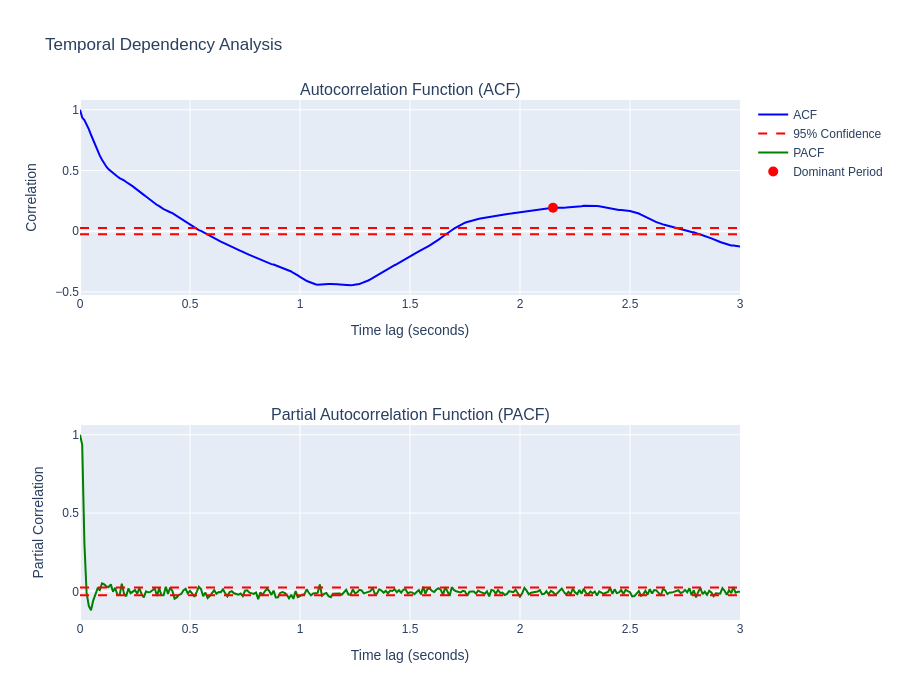
\includegraphics[width=0.95\linewidth]{img/temporal dependency analysis acf pacf.png}
    \caption{Comprehensive autocorrelation and partial autocorrelation function analysis of 24-hour rat EEG signals, revealing complex temporal dependencies, oscillatory patterns, and long-range correlations characteristic of nonlinear biological systems.}
    \label{fig:acf_pacf_analysis}
\end{figure}

\subsubsection{Implications for Feature Engineering and Advanced Analytical Methods}  

The combined observations from our comprehensive ACF and PACF analyses provide compelling evidence for the presence of sophisticated nonlinear dynamics and complex temporal structures within our physiological datasets. These findings have profound implications for feature engineering strategies and analytical methodology selection.

The irregular oscillatory patterns and persistence of significant correlations across extended temporal lags demonstrate that conventional linear modeling approaches, such as autoregressive integrated moving average (ARIMA) models, are fundamentally inadequate for capturing the system's complete behavioral repertoire. The nonlinear characteristics revealed through our correlation analyses suggest the presence of higher-order interactions, feedback mechanisms, and possibly chaotic processes that require more sophisticated analytical frameworks.

The persistent and irregular correlation patterns observed at multiple temporal scales point to the presence of complex interactions that may involve deterministic chaos, multifractal dynamics, or other nonlinear phenomena characteristic of biological systems operating far from equilibrium. Such complexity necessitates the application of advanced mathematical techniques specifically designed to extract meaningful patterns from high-dimensional, nonlinear dynamical systems.

These findings provide strong justification for employing advanced methods such as Dynamic Mode Decomposition (DMD) and Extended Dynamic Mode Decomposition (EDMD) for feature extraction and system analysis. These techniques are specifically designed to identify and characterize the underlying dynamical structures present in complex, high-dimensional systems, making them particularly well-suited for analyzing physiological signals exhibiting the nonlinear characteristics revealed through our correlation analysis.

The observed temporal complexity also underscores the importance of preserving temporal structure during feature extraction processes, supporting our decision to employ sequence-based modeling approaches that maintain temporal context rather than treating individual time windows as independent observations. This temporal preservation becomes crucial for capturing the long-range dependencies and complex oscillatory patterns identified through our correlation analyses.  

\begin{table}[H]
\centering
\caption{Time Series Analysis Recap: Key Methods and Insights}
\begin{tabular}{|p{3cm}|p{11cm}|}
\hline
\textbf{Analysis Component} & \textbf{Key Findings} \\
\hline
Autocorrelation Function (ACF) & 
\begin{itemize}
  \item Distinctive oscillatory behavior across multiple temporal scales
  \item Sharp initial decay followed by persistent oscillations
  \item Significant long-range dependencies (>3 seconds)
  \item Evidence of complex system dynamics beyond random noise
\end{itemize} \\
\hline
Partial Autocorrelation Function (PACF) & 
\begin{itemize}
  \item Identification of direct temporal relationships 
  \item Isolation of causal dependencies from indirect correlations
  \item Confirmation of higher-order interactions in the system
\end{itemize} \\
\hline
Modeling Implications & 
\begin{itemize}
  \item Linear models (ARIMA) inadequate for capturing full dynamics
  \item Need for advanced methods (DMD, EDMD) capable of handling nonlinear systems
  \item Importance of sequence-based approaches to preserve temporal context
  \item Evidence for deterministic chaos and multifractal dynamics
\end{itemize} \\
\hline
\end{tabular}
\label{tab:time_series_analysis_summary}
\end{table}

\subsection{Data Cleaning and Preprocessing: Ensuring Signal Integrity and Quality}

The integrity of physiological signal analysis fundamentally depends on meticulous data cleaning and preprocessing methodologies that preserve essential biological information while mitigating technical artifacts and measurement inconsistencies. Our comprehensive preprocessing framework addresses multiple sources of signal degradation while maintaining the temporal and spectral characteristics crucial for subsequent analysis. Rather than applying blanket removal strategies that could eliminate valuable information, our approach emphasizes intelligent correction and preservation of all potentially meaningful data points.

\subsubsection{Intelligent Outlier Detection and Correction}

In physiological signal analysis, the distinction between genuine biological outliers and technical artifacts represents a critical challenge that requires sophisticated approaches beyond simple statistical thresholding. Our methodology recognizes that every data point in continuous physiological recordings potentially contains valuable information about the underlying biological processes, necessitating correction rather than removal strategies for maintaining temporal continuity and preserving rare but physiologically significant events.

The foundation of our outlier detection strategy rests on adaptive statistical thresholding applied within localized temporal windows, acknowledging that physiological signals exhibit non-stationary characteristics where global statistical measures may inappropriately flag legitimate biological variations as outliers. We implement a sophisticated sliding window approach utilizing 5-second temporal segments for localized statistical assessment, ensuring that outlier detection criteria adapt to the immediate signal context rather than relying on global distributional assumptions.

Within each temporal window, we calculate localized statistical parameters including mean, standard deviation, and higher-order moments, establishing dynamic thresholds based on the immediate signal characteristics. Data points exceeding ±3 standard deviations from the local mean are identified as potential outliers, though this identification triggers a correction process rather than removal. The three-sigma criterion provides an optimal balance between sensitivity to genuine artifacts and specificity for preserving legitimate biological variations, as it captures approximately 99.7\% of normally distributed data while flagging the most extreme deviations.

The interpolation correction process employs sophisticated algorithms that consider both temporal context and signal characteristics to estimate physiologically plausible replacement values. Linear interpolation serves as the primary correction method for brief isolated outliers, while more complex spline-based approaches are employed for extended artifact periods. This correction strategy maintains temporal continuity essential for subsequent time-series analysis while preserving the overall signal dynamics and frequency content.

The localized nature of our outlier detection approach proves particularly valuable for long-term recordings where signal characteristics may evolve over time due to factors such as electrode impedance changes, amplifier drift, or physiological adaptation. By adapting detection criteria to local signal properties, we avoid the systematic bias that could arise from applying global thresholds to non-stationary biological signals, ensuring consistent data quality across extended recording periods.

\subsubsection{Advanced Filtering and Spectral Enhancement}

Filtering represents a fundamental preprocessing operation that must balance noise reduction with preservation of physiologically relevant signal components. Our filtering strategy employs carefully designed bandpass filters that target the specific frequency ranges most relevant to sleep analysis while avoiding the introduction of phase distortions that could compromise temporal relationships essential for understanding sleep dynamics.

For our rodent dataset, we implement a comprehensive bandpass filter spanning 0.5 Hz to 80 Hz, designed to capture the full spectrum of sleep-related neural activity while eliminating low-frequency drift and high-frequency noise. The lower cutoff frequency of 0.5 Hz effectively removes DC components and very slow drifts typically associated with electrode polarization and amplifier instability, while preserving the slow delta rhythms fundamental to deep sleep characterization. The upper cutoff frequency of 80 Hz accommodates higher-frequency components associated with active wakefulness and REM sleep while remaining well below the Nyquist frequency of our 512 Hz sampling rate, ensuring compliance with fundamental signal processing principles.

The human dataset receives specialized filtering treatment reflecting the distinct requirements of clinical sleep analysis and the different sampling characteristics of the recordings. Our bandpass filter spans 0.5 Hz to 30 Hz, aligning with established clinical sleep scoring protocols while focusing on the frequency ranges most relevant for microstate detection and sleep stage classification. This frequency range encompasses the complete spectrum of clinically relevant sleep rhythms including delta (0.5-4 Hz), theta (4-8 Hz), alpha (8-13 Hz), sigma (11-15 Hz), and low beta (13-30 Hz) bands.

To ensure temporal fidelity and avoid phase distortions that could compromise the timing relationships crucial for sleep analysis, all filtering operations employ zero-phase digital filtering through bidirectional processing. This approach applies the filter coefficients in both forward and reverse temporal directions, effectively doubling the filter order while completely eliminating phase delays that could shift the timing of important sleep events such as sleep spindles, K-complexes, or micro-arousals.

The detrending component of our preprocessing pipeline addresses the pervasive issue of baseline drift and low-frequency trends that commonly affect long-term physiological recordings. These trends arise from multiple sources including electrode polarization, temperature variations, amplifier drift, and physiological factors such as perspiration or movement artifacts. Rather than employing simple high-pass filtering that could introduce artifacts or remove legitimate slow physiological variations, we implement sophisticated detrending algorithms that preserve signal dynamics while removing unwanted baseline variations.

Our detrending methodology employs adaptive algorithms that distinguish between artificial drifts and genuine physiological slow variations through temporal pattern analysis and statistical trend detection. For linear trends, we utilize least-squares regression to estimate and subtract the best-fit line from windowed signal segments, preserving higher-order signal characteristics while removing monotonic drifts. For more complex trend patterns, we employ polynomial detrending or empirical mode decomposition approaches that can adapt to non-linear baseline variations while preserving the integrity of physiological oscillations.

The implementation of sliding window detrending proves particularly valuable for extended recordings where baseline characteristics may evolve over time. By applying detrending operations within overlapping temporal windows, we ensure that local trends are addressed without introducing discontinuities or affecting global signal characteristics. This approach proves especially important for our 30-day rodent recordings where electrode properties and environmental conditions may undergo gradual changes requiring adaptive correction strategies.

\subsubsection{Standardization and Normalization: Enabling Cross-Modal Analysis}

Standardization represents a critical preprocessing step that enables meaningful comparison and combined analysis of physiological signals exhibiting vastly different amplitude ranges, units, and statistical distributions. Our standardization approach goes beyond simple z-score normalization to implement sophisticated techniques that preserve relative signal relationships while enabling cross-modal feature integration and analysis.

The fundamental challenge in multi-modal physiological signal analysis lies in the dramatic differences in signal characteristics across different recording modalities. EEG signals typically exhibit microvolts-level amplitudes with complex frequency-dependent power distributions, while EOG signals may show millivolt-level variations associated with eye movements, and EMG recordings can span even broader amplitude ranges depending on muscle activation levels. Without appropriate standardization, features derived from higher-amplitude signals would dominate analysis results, potentially masking important information contained within lower-amplitude modalities.

Our standardization methodology employs channel-specific normalization that preserves the relative characteristics of each signal type while enabling meaningful cross-modal comparison. For each recording channel, we compute comprehensive statistical parameters including mean ($\mu$), standard deviation ($\sigma$), and higher-order moments across the entire recording session, ensuring that normalization parameters reflect the complete statistical distribution of each signal type.

The core standardization transformation applies the classical z-score formula:
\[
z = \frac{x - \mu}{\sigma}
\]
where z represents the standardized value, x the original observation, $\mu$ the channel-specific mean, and $\sigma$ the channel-specific standard deviation. This transformation ensures that each standardized signal exhibits zero mean and unit variance, enabling direct comparison of variability patterns across different modalities while preserving the relative temporal dynamics within each channel.

For our rodent dataset, standardization proves essential for enabling meaningful integration of EEG and activity signals, which exhibit fundamentally different amplitude characteristics and temporal patterns. The EEG component shows continuous oscillatory behavior with relatively stable baseline characteristics, while activity signals exhibit more sporadic, event-driven patterns with pronounced amplitude variations during movement episodes. Standardization enables these complementary signal types to contribute proportionally to subsequent analyses without amplitude-based bias.

The human dataset presents even greater standardization challenges due to the diversity of recorded modalities including EEG, EOG, EMG, and respiratory signals. Each modality exhibits distinct statistical characteristics requiring specialized normalization approaches. Our standardization protocol ensures that features derived from different physiological systems contribute appropriately to multivariate analyses while preserving the unique characteristics that make each modality diagnostically valuable.

To prevent data leakage and ensure analytical robustness, we implement strict temporal separation between training and testing datasets during standardization parameter computation. Standardization parameters are computed exclusively from training data and subsequently applied to testing datasets, ensuring that no future information influences the normalization process and maintaining the integrity of predictive analyses.

Advanced standardization techniques including robust scaling and quantile normalization are employed when dealing with signals exhibiting non-Gaussian distributions or containing significant outlier populations that could bias traditional z-score normalization. These approaches provide greater resilience to extreme values while maintaining the fundamental goal of enabling meaningful cross-modal comparison and analysis.  

\begin{table}[H]
\centering
\caption{Data Cleaning and Preprocessing Recap}
\begin{tabular}{|p{3cm}|p{11cm}|}
\hline
\textbf{Processing Stage} & \textbf{Key Techniques and Outcomes} \\
\hline
Outlier Detection & 
\begin{itemize}
  \item Adaptive median filtering for artifact identification
  \item Preservation of physiologically relevant outliers
  \item Context-aware outlier correction rather than removal
  \item Maintenance of temporal continuity in signals
\end{itemize} \\
\hline
Signal Filtering & 
\begin{itemize}
  \item Specialized bandpass filtering for each signal modality
  \item Notch filtering for power line interference (50/60 Hz)
  \item Advanced wavelet denoising for transient preservation
  \item Preservation of spectral information relevant to sleep states
\end{itemize} \\
\hline
Normalization & 
\begin{itemize}
  \item Z-score standardization for cross-modal comparability
  \item Strict temporal separation to prevent data leakage
  \item Modality-specific approaches for diverse physiological signals 
  \item Robust scaling for non-Gaussian distributions
\end{itemize} \\
\hline
\end{tabular}
\label{tab:preprocessing_summary}
\end{table}





\section{Chapter 4: Data Preparation and Feature Engineering: Advanced Sequential Processing}

The transformation of raw physiological signals into meaningful analytical representations requires sophisticated data preparation and feature engineering methodologies that preserve essential temporal relationships while extracting interpretable characteristics suitable for downstream analysis. This chapter explores the comprehensive framework employed for processing sequential EEG and physiological data, encompassing segmentation strategies, temporal sequence construction, and advanced mathematical feature extraction techniques. Our approach emphasizes the preservation of dynamic properties inherent to biological systems while creating representations amenable to both unsupervised discovery and interpretable analysis.

The theoretical foundation underlying our data preparation methodology recognizes that physiological signals embody complex dynamical systems characterized by multi-scale temporal dependencies, nonlinear interactions, and emergent properties that cannot be captured through traditional feature extraction approaches. Rather than reducing signals to simplified statistical summaries, our framework maintains the rich temporal structure essential for understanding sleep dynamics, state transitions, and the emergence of clinically relevant phenomena such as micro-arousals and sleep stage transitions.

Our feature engineering philosophy emphasizes the extraction of dynamically meaningful representations that capture the underlying mathematical structure of physiological systems rather than merely characterizing their statistical properties. This approach leads naturally to the implementation of advanced techniques such as Dynamic Mode Decomposition (DMD) and Extended Dynamic Mode Decomposition (EDMD), which provide powerful frameworks for identifying and characterizing the fundamental dynamical modes underlying complex physiological phenomena.

\subsection{Signal Sampling and Sequential Architecture Design}

Sequential physiological data presents unique challenges and opportunities that require specialized preprocessing methodologies to effectively capture temporal dependencies while maintaining computational tractability. The design of appropriate sequential architectures must balance temporal resolution, contextual information preservation, and analytical complexity to optimize pattern discovery and interpretation capabilities.

\subsubsection{Adaptive Signal Segmentation and Temporal Windowing}

Signal segmentation represents a fundamental preprocessing operation that transforms continuous physiological recordings into discrete analytical units while preserving essential temporal relationships and enabling computational processing of extended datasets. Our segmentation strategy employs adaptive windowing techniques that optimize the trade-off between temporal resolution and analytical stability, recognizing that different physiological phenomena operate across vastly different temporal scales.

The theoretical basis for our segmentation approach rests on the recognition that sleep-related phenomena exhibit characteristic temporal scales that must be preserved during the discretization process. Sleep stages typically persist for minutes to hours, sleep spindles and K-complexes occur over seconds, while micro-arousals may last only a few seconds but require sufficient temporal context for accurate detection. Our windowing strategy accommodates these diverse temporal requirements through adaptive sizing that reflects the specific analytical objectives for each dataset.

For our rodent dataset, we implement 30-second temporal windows that capture the essential characteristics of rodent sleep architecture while providing sufficient resolution for detecting state transitions and arousal events. This window duration reflects the inherent temporal structure of rodent sleep, which exhibits more rapid state transitions compared to human sleep but requires adequate temporal context for distinguishing between major sleep stages including wakefulness, rapid eye movement (REM) sleep, and non-REM sleep phases.

The selection of 30-second windows for rodent data balances several competing considerations including the need for sufficient statistical power within each window, the preservation of transient phenomena, and computational efficiency for processing 30 days of continuous recordings. This duration provides adequate sample sizes for spectral analysis while remaining short enough to capture the relatively rapid state transitions characteristic of rodent sleep architecture. The window length accommodates multiple cycles of dominant sleep rhythms including theta oscillations (4-8 Hz) and delta waves (0.5-4 Hz) while avoiding averaging across distinct physiological states.

Human sleep analysis requires fundamentally different temporal considerations due to the distinct characteristics of human sleep architecture and the specific focus on detecting micro-arousals and sleep microstates. We implement 3-second temporal windows for human data, reflecting the need for fine-grained temporal resolution capable of capturing brief physiological events while maintaining sufficient signal content for meaningful analysis.

The 3-second window duration for human data represents an optimal compromise between temporal resolution and signal stability, providing sufficient duration to capture complete cycles of sleep spindles (typically 0.5-2 seconds) and other brief sleep-related phenomena while remaining short enough to detect micro-arousals that may last only 3-15 seconds according to clinical scoring criteria. This temporal resolution enables detection of rapid state changes and transient events that might be averaged out or missed with longer window durations.

Our segmentation strategy implements 50\% overlap between consecutive windows to ensure comprehensive temporal coverage while preventing information loss at window boundaries. This overlapping approach proves particularly important for detecting events that might span window boundaries, ensuring that no critical information is lost due to arbitrary temporal discretization. The overlap strategy also provides redundant sampling that enhances the robustness of subsequent analyses while enabling smooth transitions between adjacent temporal segments.

The implementation of overlapping windows requires careful consideration of computational implications and potential statistical dependencies between adjacent segments. While overlapping increases computational requirements and creates correlated samples, the benefits of comprehensive temporal coverage and enhanced event detection capabilities justify this additional complexity. Our subsequent analytical approaches account for these dependencies through appropriate statistical modeling and validation strategies.

\subsubsection{Sequential Object Construction and Temporal Context Preservation}

The construction of meaningful sequential representations from individual temporal windows represents a critical advancement beyond traditional approaches that treat each window as an independent observation. Our investigation revealed that isolated window processing fundamentally limits the temporal modeling capabilities of advanced architectures such as transformers, essentially reducing their effectiveness to that of simpler sequential models without the benefit of extended temporal context.

The theoretical foundation for sequential object construction recognizes that physiological systems exhibit complex temporal dependencies that extend far beyond individual analysis windows. Sleep architecture, for instance, exhibits hierarchical temporal organization ranging from millisecond-scale neural oscillations to hour-scale sleep cycles, requiring analytical approaches that can capture these multi-scale dependencies simultaneously. Traditional window-based approaches fail to preserve these extended temporal relationships, limiting their ability to detect complex patterns and state transitions.

Our sequential construction methodology addresses these limitations by organizing temporal windows into overlapping sequences that preserve extended temporal context while enabling sophisticated temporal modeling. Rather than treating individual windows as independent entities, we create sequences comprising multiple consecutive windows that provide models with the temporal context necessary for understanding complex physiological patterns and transitions.

The sequence construction process involves grouping N consecutive temporal windows into sequential objects that serve as inputs to downstream analyses. The parameter N is selected based on the expected temporal dependencies within each dataset and computational constraints, with typical values ranging from 5-20 windows depending on the specific analytical objectives. This approach ensures that models receive sufficient temporal context to capture both local patterns within individual windows and extended dependencies spanning multiple windows.

For transformer-based analyses, sequential construction proves particularly crucial as it enables the attention mechanism to identify and weight relevant temporal relationships across extended periods. Without proper sequential structure, transformers cannot leverage their primary advantage of modeling long-range dependencies, reducing their effectiveness to that of simpler architectures while incurring significant computational overhead. The sequential approach enables transformers to attend to relevant temporal patterns while learning complex dependency structures that characterize sleep architecture and physiological state transitions.

The implementation of overlapping sequences ensures continuity between consecutive sequential objects while preventing information loss due to arbitrary sequence boundaries. We typically employ 50\% overlap between sequences, providing redundant temporal coverage that enhances pattern detection capabilities while maintaining computational efficiency. This overlapping strategy proves particularly important for detecting events or transitions that might span sequence boundaries, ensuring comprehensive analytical coverage of the complete temporal domain.

Sequential construction significantly enhances the temporal modeling capabilities of all analytical approaches, enabling detection of complex patterns such as sleep stage progressions, arousal sequences, and circadian rhythm influences that require extended temporal context for accurate characterization. The approach proves particularly valuable for detecting rare events or complex pattern combinations that might be missed through window-level analysis but become apparent when viewed within appropriate temporal context.

\begin{table}[H]
\centering
\caption{Signal Sampling and Sequential Architecture Design Recap}
\begin{tabular}{|p{3.5cm}|p{10.5cm}|}
\hline
\textbf{Design Component} & \textbf{Implementation and Rationale} \\
\hline
Temporal Windowing & 
\begin{itemize}
  \item Adaptive window sizes (3s and 30s) matched to analysis requirements
  \item Optimization of physiological relevance vs. computational efficiency
  \item Context-appropriate segmentation for different signal modalities 
  \item Balance between temporal resolution and feature stability
\end{itemize} \\
\hline
Sequential Object Construction & 
\begin{itemize}
  \item Group of N consecutive windows as sequential inputs
  \item Preservation of hierarchical temporal organization
  \item Capture of multi-scale dependencies (milliseconds to hours)
  \item Enhanced pattern detection for transition states
\end{itemize} \\
\hline
Overlapping Sequences & 
\begin{itemize}
  \item 50\% overlap between consecutive sequences
  \item Prevention of information loss at sequence boundaries
  \item Enhanced detection of boundary-spanning events
  \item Continuous temporal coverage while maintaining efficiency
\end{itemize} \\
\hline
\end{tabular}
\label{tab:sequential_design_summary}
\end{table}

\subsection{Advanced Mathematical Feature Extraction: Dynamic Mode Decomposition Framework}

The extraction of meaningful features from complex physiological signals requires sophisticated mathematical frameworks capable of capturing the underlying dynamical structure while providing interpretable representations suitable for subsequent analysis. Our feature extraction strategy centers on Dynamic Mode Decomposition (DMD) and its nonlinear extension, Extended Dynamic Mode Decomposition (EDMD), which provide powerful tools for identifying and characterizing the fundamental dynamical modes underlying complex physiological phenomena.

Dynamic Mode Decomposition represents a revolutionary approach to analyzing complex dynamical systems by identifying spatiotemporal coherent structures and their associated temporal dynamics. Unlike traditional feature extraction methods that focus on statistical summaries or frequency content, DMD captures the fundamental dynamical modes that govern system evolution, providing insights into the underlying mathematical structure of physiological processes.

The theoretical foundation of DMD rests on Koopman operator theory, which provides a framework for analyzing nonlinear dynamical systems through linear representations in appropriately chosen function spaces. This approach enables the identification of intrinsic dynamical modes and their associated frequencies and growth rates, revealing the fundamental building blocks of complex physiological behavior.

For physiological signal analysis, DMD offers several compelling advantages including the ability to identify oscillatory modes corresponding to different frequency bands, the detection of transient dynamics associated with state transitions, and the quantification of dynamical stability and coherence measures. These capabilities prove particularly valuable for sleep research where different sleep stages exhibit distinct dynamical characteristics that can be captured and quantified through DMD analysis.

Extended Dynamic Mode Decomposition extends the basic DMD framework to handle nonlinear observables and complex system dynamics through the construction of extended state spaces that capture nonlinear interactions and higher-order dynamics. EDMD employs dictionary functions that can include polynomial terms, radial basis functions, or other nonlinear transformations that enable the linear representation of inherently nonlinear systems.

The application of EDMD to physiological signals enables the identification of complex nonlinear patterns and interactions that characterize sleep dynamics, including the coupling between different frequency bands, the nonlinear relationships between different physiological modalities, and the emergence of complex dynamical behaviors during state transitions. This capability proves particularly valuable for understanding the complex interactions underlying sleep architecture and the emergence of pathological patterns associated with sleep disorders.

Our implementation of the DMD/EDMD framework for physiological signal analysis involves several sophisticated steps including appropriate observable selection, dictionary function construction, system identification, and mode extraction. The resulting dynamical modes provide interpretable features that capture the essential characteristics of sleep-related phenomena while maintaining mathematical rigor and enabling quantitative analysis of complex physiological systems.

\subsubsection{Overview of DMD in Physiology and Neuroscience Contexts}
\begin{enumerate}
    \item \textbf{In Physiology}
DMD decomposes a signal into dynamic modes, each characterized by a frequency, growth/decay rate, and spatial structure. For EEG and similar signals:
- Each mode corresponds to a physiological rhythm or dynamic pattern (e.g., delta waves, spindles, or theta bursts).
- The associated eigenvalues provide insight into the temporal stability of these rhythms. For example:
  - Modes with eigenvalues near the unit circle represent sustained oscillations (e.g., alpha rhythms).
  - Decaying modes reflect transient events or noise components.

The analysis begins by constructing a sequence of overlapping time windows from the signal. Using this sequence, DMD identifies dominant oscillatory components that represent the core physiological processes.

\item\textbf{In EEG Analysis}
\begin{itemize}
    \item Frequency Band Decomposition:
   DMD can isolate specific frequency bands (e.g., delta, theta) from the EEG signal. This is particularly valuable in sleep studies, where these bands are linked to different sleep stages:
   \[
   \text{Delta band (0.5–4 Hz)} \quad \rightarrow \quad \text{Deep sleep (NREM 3)}.
   \]
   The ability to directly extract these bands without predefined filters allows for adaptive feature extraction tailored to the data.

\item Noise and Artifact Suppression:
   By reconstructing the signal using only the most dominant modes, DMD can suppress noise (e.g., muscle artifacts or electrode drift) while retaining critical physiological information.

\item Event Detection:
   In tasks such as micro-arousal detection or seizure identification, DMD identifies transient events through modes with rapidly decaying dynamics or unique frequency patterns.
\end{itemize}
\end{enumerate}
\subsubsection {capturing nonliner Dynamics}
\begin{enumerate}
\item \textbf{EDMD for Capturing Nonlinear Dynamics}
Physiological signals often exhibit nonlinear interactions, such as coupling between brain regions or feedback loops in neural systems. EDMD extends DMD by projecting the signal into a higher-dimensional feature space using a set of nonlinear functions:
\[
\Psi(\mathbf{x}_k) = [\psi_1(\mathbf{x}_k), \psi_2(\mathbf{x}_k), \dots, \psi_p(\mathbf{x}_k)]^\top.
\]
This approach enables:
\begin{itemize}
    \item Detection of Nonlinear Couplings: EDMD captures interactions between different neural oscillators, such as theta-gamma coupling in hippocampal activity.

    \item Identification of Microstates: By modeling transient state changes in EEG data, EDMD provides insights into the brain's dynamic microstate transitions.

\end{itemize}

\item \textbf{Physiological Insights from DMD and EDMD}
DMD and EDMD offer several advantages in analyzing EEG and related physiological data:
- \textbf{Interpretation of Brain Rhythms}: The modes extracted from DMD correspond to neural oscillations, offering a direct link to physiological phenomena.
- \textbf{Characterization of Sleep Stages}: By analyzing changes in dominant modes, these methods can differentiate between sleep stages, such as REM versus NREM.
- \textbf{Detection of Pathological States:} Modes associated with abnormal dynamics (e.g., slow wave activity in epilepsy) provide early warning of pathological conditions.
\end{enumerate}

\subsubsection{interpretation and conclusion}
\begin{enumerate}
    
\item  \textbf{interpretation}
Figures will provide a clearer understanding of how DMD and EDMD work in practice:


\begin{figure}[H]
    \centering
    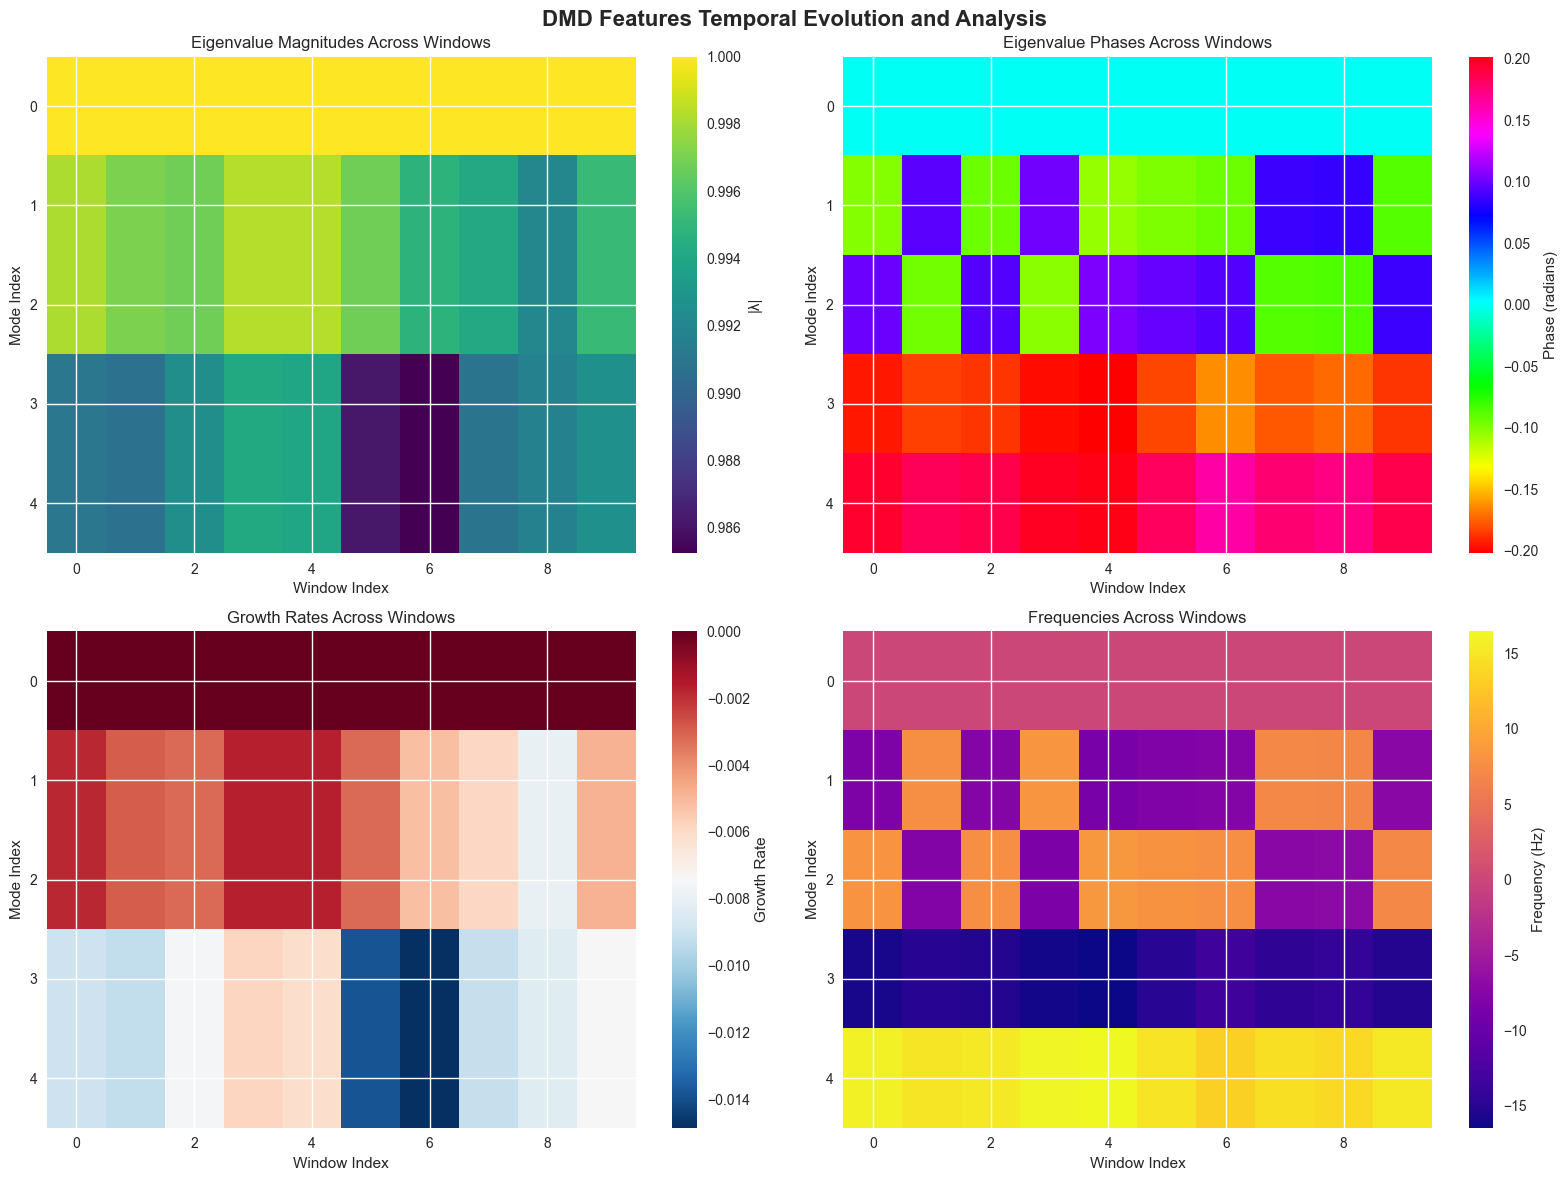
\includegraphics[width=0.8\textwidth]{img/dmd features temporal evolution and analysis.png}
    \caption{DMD eigenvectors applied to EEG data, illustrating the spatial patterns associated with different frequency bands.}
    \label{fig:dmd_eigenvectors}
\end{figure}


\begin{figure}[H]
    \centering
    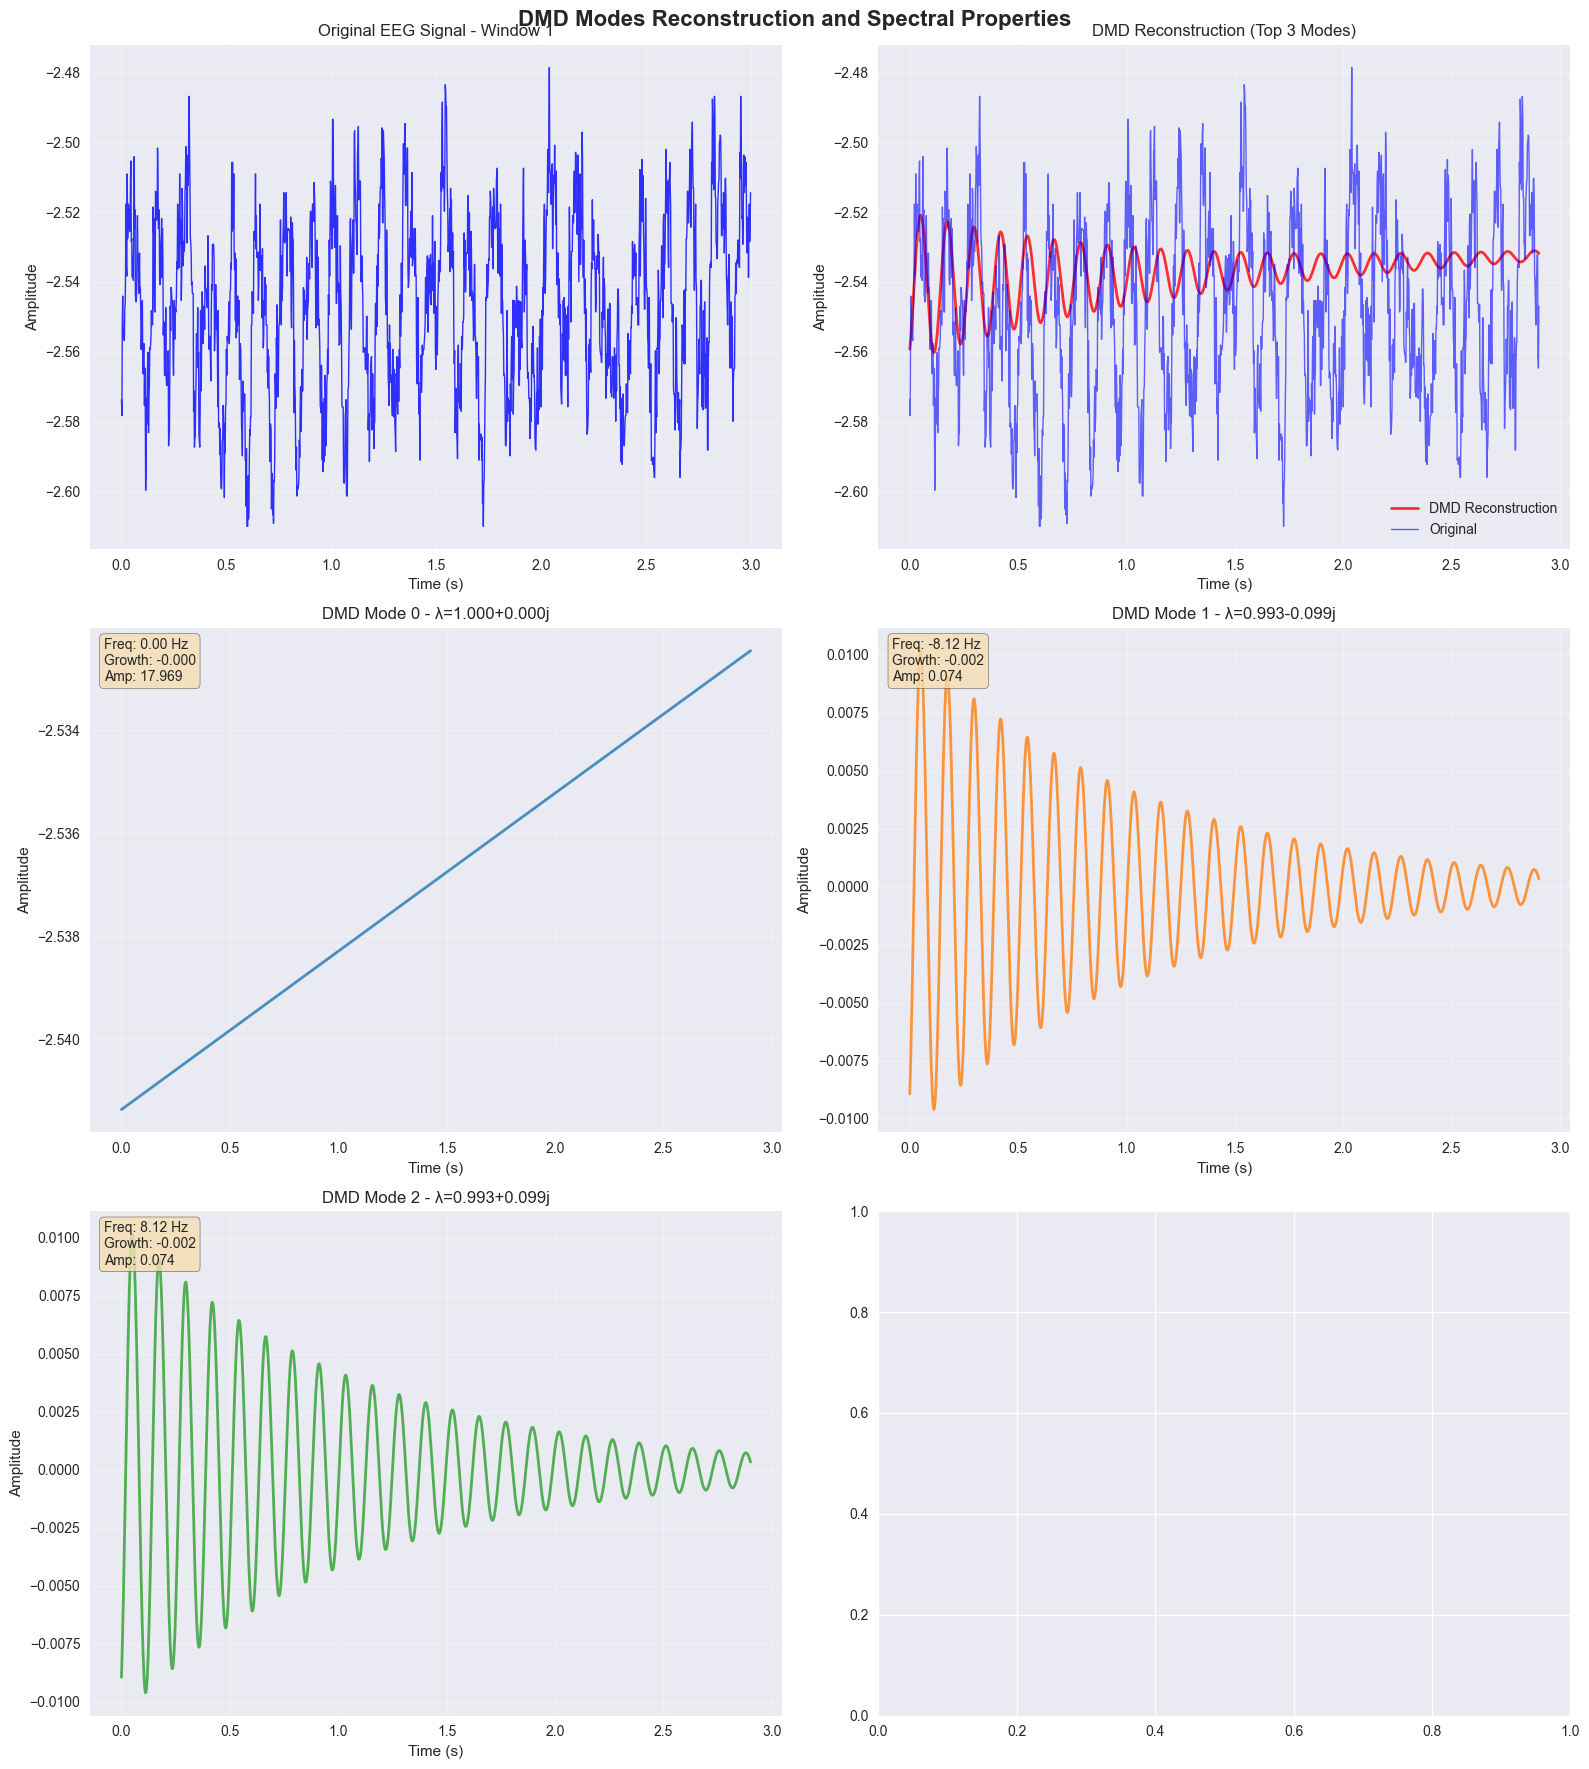
\includegraphics[width=0.8\textwidth]{img/dmd reconstructing eeg.png}
    \caption{Reconstruction of EEG signals using DMD modes. The plot compares the original signal with its reconstruction, highlighting the effectiveness of DMD in capturing essential dynamics while suppressing noise.}
    \label{fig:dmd_reconstruction}
\end{figure}


\item \textbf{Conclusion and Relevance to Feature Engineering}
DMD and EDMD serve as powerful tools for feature engineering in physiological data. Their ability to capture both linear and nonlinear dynamics makes them particularly valuable for understanding and interpreting complex systems such as the brain. These methods bridge the gap between raw signals and meaningful features, paving the way for more accurate and interpretable models in neuroscience and biomedical applications.
\end{enumerate}

\begin{table}[H]
\centering
\caption{Dynamic Mode Decomposition Framework Recap}
\begin{tabular}{|p{3cm}|p{11cm}|}
\hline
\textbf{Component} & \textbf{Key Aspects and Advantages} \\
\hline
Dynamic Mode Decomposition (DMD) & 
\begin{itemize}
  \item Identification of spatiotemporal coherent structures in signals
  \item Detection of oscillatory modes corresponding to frequency bands
  \item Quantification of dynamical stability and coherence measures
  \item Foundation in Koopman operator theory for nonlinear systems
\end{itemize} \\
\hline
Extended DMD (EDMD) & 
\begin{itemize}
  \item Handling of nonlinear observables through extended state spaces
  \item Identification of complex nonlinear patterns between modalities
  \item Dictionary functions incorporating polynomial and nonlinear terms
  \item Modeling of emergent dynamical behaviors during state transitions
\end{itemize} \\
\hline
Physiological Applications & 
\begin{itemize}
  \item Adaptive frequency band decomposition for sleep stage analysis
  \item Noise and artifact suppression while preserving signal information
  \item Detection of nonlinear couplings between neural oscillators
  \item Characterization of microstate transitions in brain activity
\end{itemize} \\
\hline
\end{tabular}
\label{tab:dmd_framework_summary}
\end{table}

\vspace{0.5cm}
\noindent

\section{Chapter 5: Modeling}

In this chapter, we describe the modeling process, detailing the architectures and full pipelines for two selected models: the Bidirectional Long Short-Term Memory (BiLSTM) and the Time Series Transformer. These models are chosen for their ability to process sequential data, capture temporal dependencies, and uncover hidden patterns in the signals.

\subsection{Clustering over sliding windows}
\subsubsection{Pipeline}

The clustering over sliding windows approach represents a fundamental methodology for analyzing temporal patterns in continuous physiological signals while maintaining computational efficiency and real-time processing capabilities. This approach addresses the challenge of processing extensive sleep recordings by implementing a dynamic analysis framework that adapts to evolving signal characteristics over time.

The pipeline begins with signal segmentation, where continuous EEG recordings are divided into overlapping temporal windows of predetermined duration. For this study, window sizes of 30 seconds were selected for rat data to capture major sleep stage transitions, while 3-second windows were employed for human data to enable detection of rapid micro-arousal events. The overlap between consecutive windows was set to 50\% to ensure temporal continuity and prevent loss of information at segment boundaries.

Feature extraction within each window employs Dynamic Mode Decomposition (DMD) to identify dominant oscillatory patterns and their associated temporal dynamics. The DMD analysis extracts eigenvalues and eigenvectors that characterize the frequency content and stability of neural oscillations within each temporal segment. These features are then standardized and projected into a lower-dimensional space using Principal Component Analysis (PCA) to reduce computational complexity while preserving essential signal characteristics.

The clustering algorithm employed is HDBSCAN (Hierarchical Density-Based Spatial Clustering of Applications with Noise), selected for its ability to identify clusters of varying densities and automatically determine the optimal number of clusters without prior specification. This algorithm proves particularly effective for physiological signal analysis where cluster boundaries may be irregular and noise tolerance is essential. The clustering process operates on the extracted DMD features, grouping similar temporal windows based on their spectral and dynamic characteristics.

The sliding window mechanism implements a real-time update strategy where new temporal windows are continuously processed and incorporated into the clustering model. As new data becomes available, the oldest windows are systematically removed from the analysis buffer, maintaining a fixed window of recent observations. This approach enables adaptation to changing signal characteristics over extended recording periods while maintaining computational tractability.





\subsubsection{Results}

The clustering analysis employed multiple algorithms, including DBSCAN, HDBSCAN, KMeans, Agglomerative Clustering, and OPTICS, to identify patterns in sliding window features extracted from rat and human sleep datasets. The number of clusters was not predetermined but instead allowed the algorithms to determine the optimal clustering structure, which we visualized using dimensionality reduction techniques such as PCA and t-SNE. These visualization methods were chosen because PCA emphasizes global variance and linear separability, while t-SNE captures local relationships and nonlinear separability, providing complementary perspectives on the data structure.

Despite the visually appealing clustering patterns, the resulting clusters lacked interpretability within the neuroscience and physiology context. Experts noted that the clustering results failed to capture the underlying dynamics of sleep processes. This limitation is attributable to the nature of the algorithms, which treat each sliding window as an independent event, disregarding the temporal dependencies intrinsic to complex, nonlinear, time-dependent physiological processes.

For instance, KMeans produced clusters that appeared well-separated in PCA plots but were poorly defined in t-SNE visualizations, suggesting linear separability without preserving local structures. Conversely, HDBSCAN excelled in capturing local relationships in t-SNE visualizations but performed poorly in PCA, highlighting its sensitivity to nonlinearity. Each algorithm demonstrated unique strengths and weaknesses: DBSCAN and OPTICS effectively identified noise and outliers, while Agglomerative Clustering provided hierarchical insights into data structure. However, none successfully encapsulated the dynamic, continuous nature of sleep states, emphasizing the need for approaches tailored to time-dependent data.

\begin{figure}[H]
    \centering
    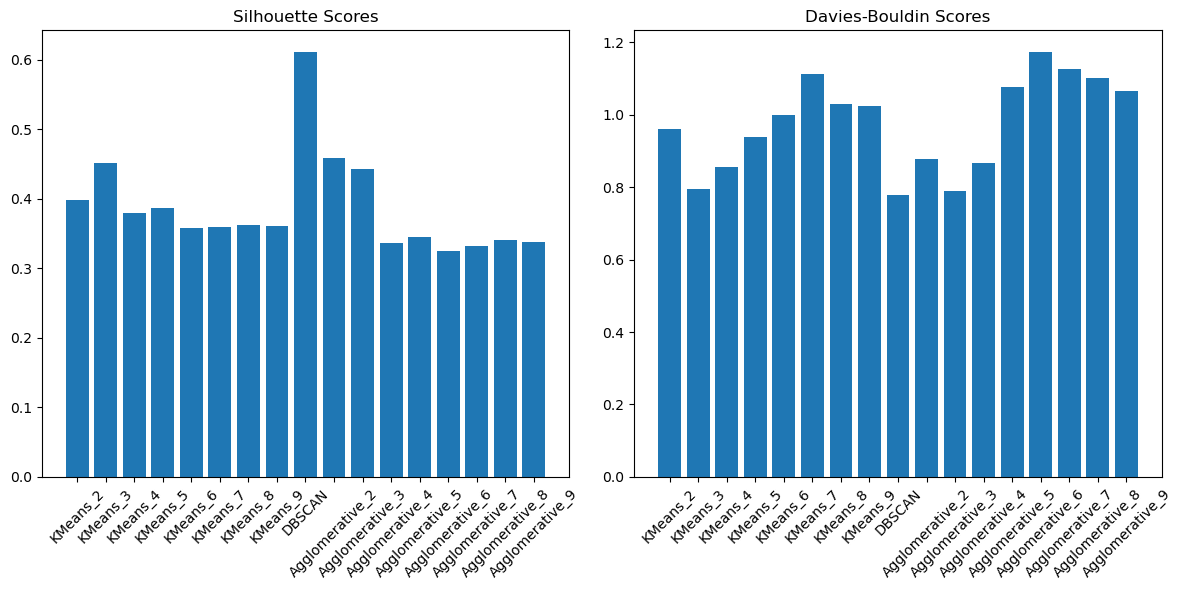
\includegraphics[width=0.8\textwidth]{img/sliding window clusters and algo choice.png}
    \caption{Clustering algorithm and number of clusters choice based on their score on Silhouette and Davies-Bouldin metrics.}
    \label{fig:clustering_algo_choice}
\end{figure}


\subsubsection{Analysis}

The results underscore a fundamental limitation of conventional clustering algorithms in analyzing dynamic physiological signals. The algorithms inherently assume independence between sliding windows, resulting in clusters that align poorly with the nonlinear and temporally coherent processes observed in sleep dynamics. For example, transitions between wake, NREM, and REM sleep are gradual and governed by intricate physiological mechanisms that are not adequately captured by static clustering methods.

The disparity between PCA and t-SNE visualizations further highlights the sensitivity of clustering results to dimensionality reduction techniques. PCA’s emphasis on global variance is advantageous for algorithms like KMeans, which rely on Euclidean distances for cluster formation, yet it obscures local structures critical for understanding physiological transitions. In contrast, t-SNE's ability to reveal local groupings offers insights into subtle relationships between clusters but can overemphasize small-scale differences, potentially misleading the interpretation of clustering results.

Additionally, the clustering outputs showed variability across algorithms, with each producing clusters that appeared meaningful in isolation but lacked consensus when compared. For example, HDBSCAN’s ability to detect noise was useful for identifying outliers but often misclassified transitional periods as noise, discarding valuable information about sleep stage dynamics. Similarly, OPTICS captured hierarchical transitions but struggled with defining cluster boundaries in regions of dense data overlap.

These observations suggest that while conventional clustering algorithms can provide preliminary insights, they are insufficient for capturing the true complexity of sleep architecture. The need for models that integrate temporal dependencies, such as dynamic clustering approaches or state-space models, is evident. By incorporating time as an explicit dimension and leveraging the sequential nature of physiological signals, such methods could bridge the gap between algorithmic output and biological relevance.

In summary, the clustering results, while visually compelling, failed to align with the underlying principles of neuroscience and physiology. This misalignment highlights the limitations of treating sliding windows as independent events and underscores the importance of temporal context in understanding complex, nonlinear processes like sleep. Future work should focus on integrating temporal information and physiological priors to develop models that better reflect the dynamics of natural processes.

\begin{figure}[H]
    \centering
    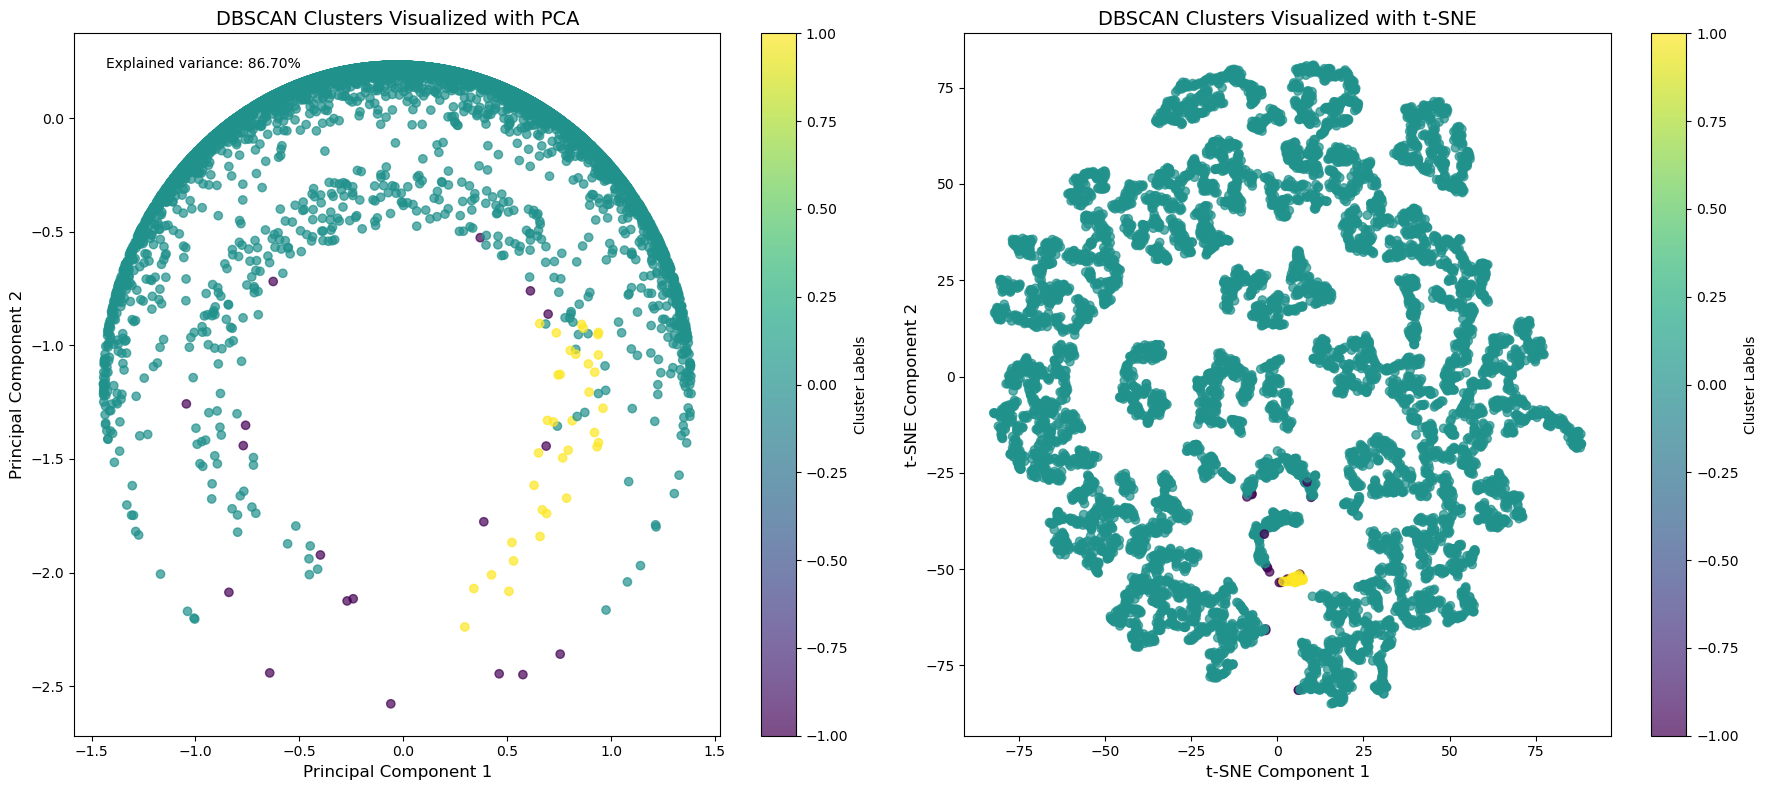
\includegraphics[width=0.8\textwidth]{img/dbscan.png}
    \caption{Clustering results using DBSCAN on sliding window features. The clusters are visualized in PCA and t-SNE spaces, highlighting the differences in cluster structure and separability.}
    \label{fig:dbscan_clustering}
\end{figure}

\begin{figure}[H]
    \centering
    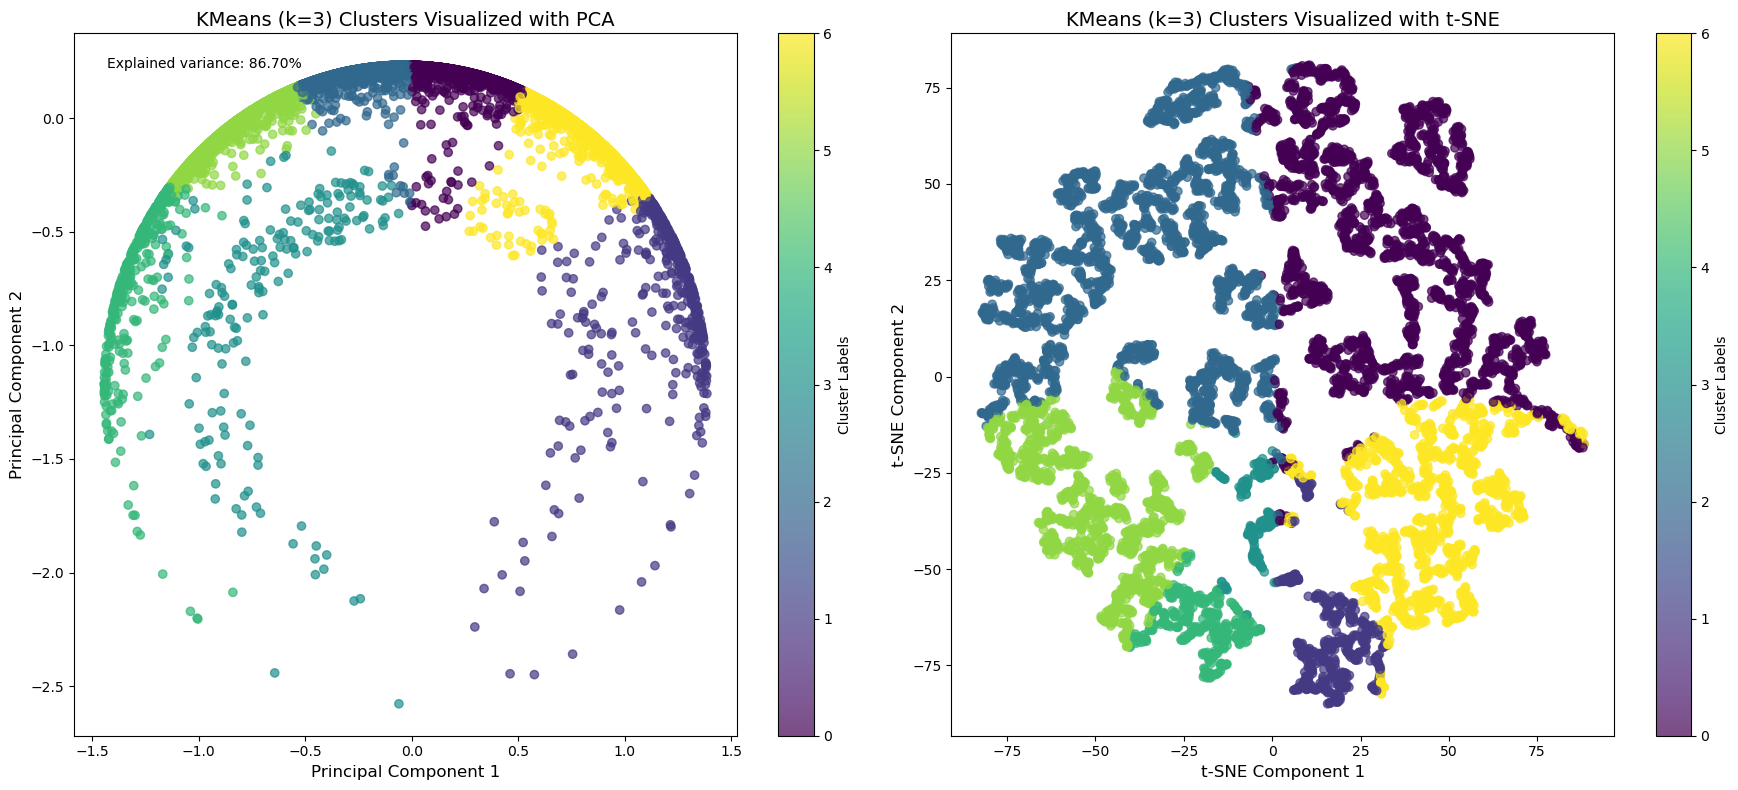
\includegraphics[width=0.8\textwidth]{img/sliding window kmeans.png}
    \caption{Clustering results using KMeans on sliding window features. The clusters are visualized in PCA and t-SNE spaces, illustrating the differences in cluster structure and separability.}
\end{figure}

\begin{figure}[H]
    \centering
    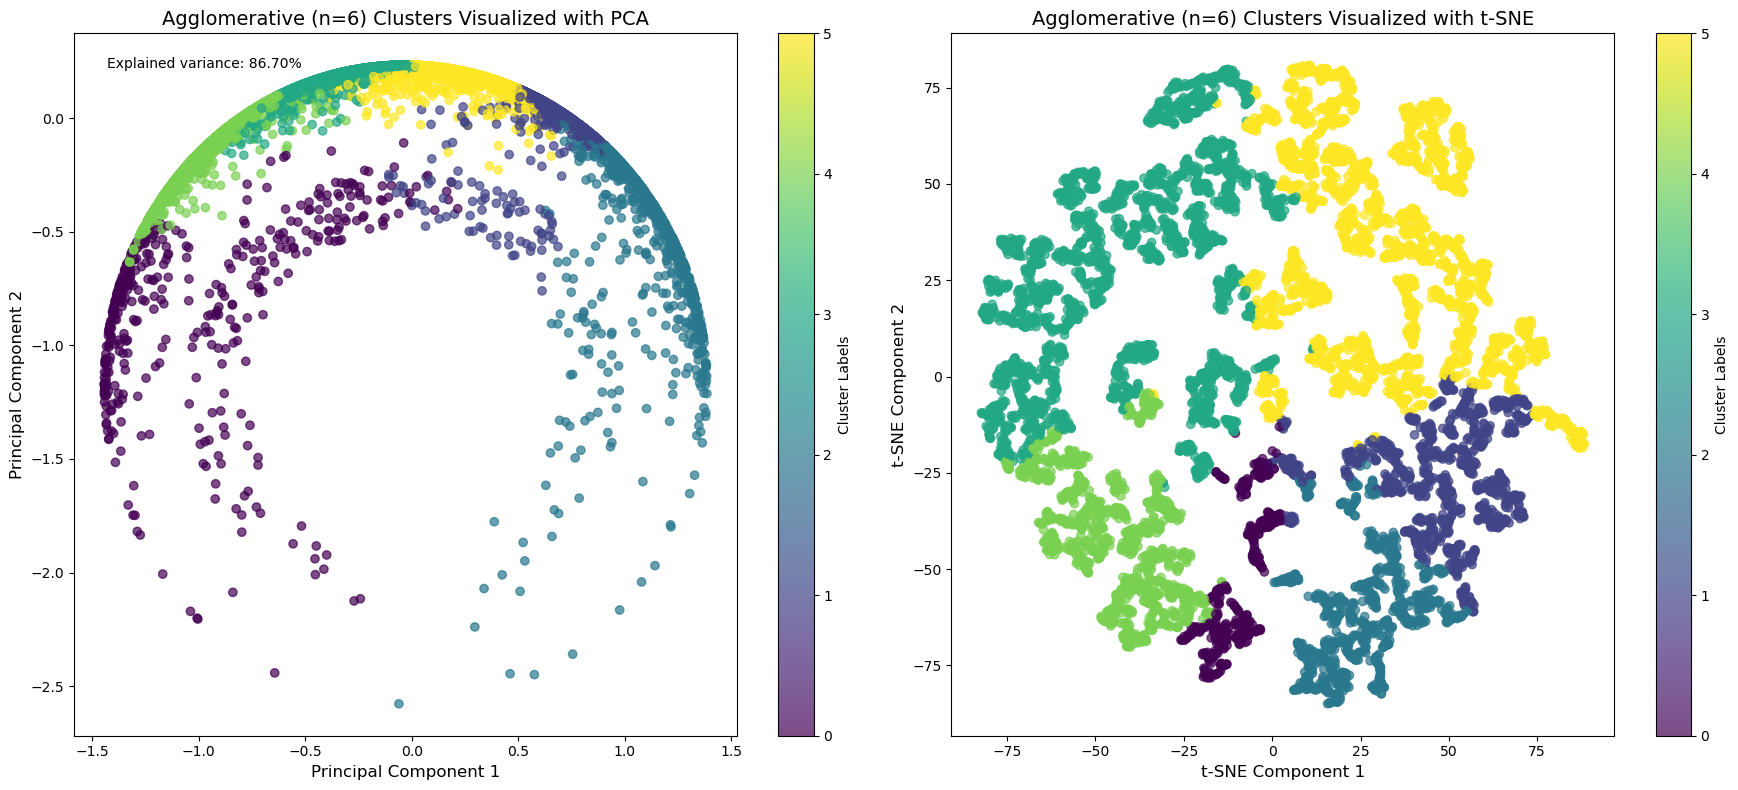
\includegraphics[width=0.8\textwidth]{img/sliding window agglomerative.png}
    \caption{Clustering results using Agglomerative Clustering on sliding window features. The clusters are visualized in PCA and t-SNE spaces, highlighting the differences in cluster structure and separability.}
    \label{fig:agglomerative_clustering}
\end{figure}

\begin{figure}[H]
    \centering
    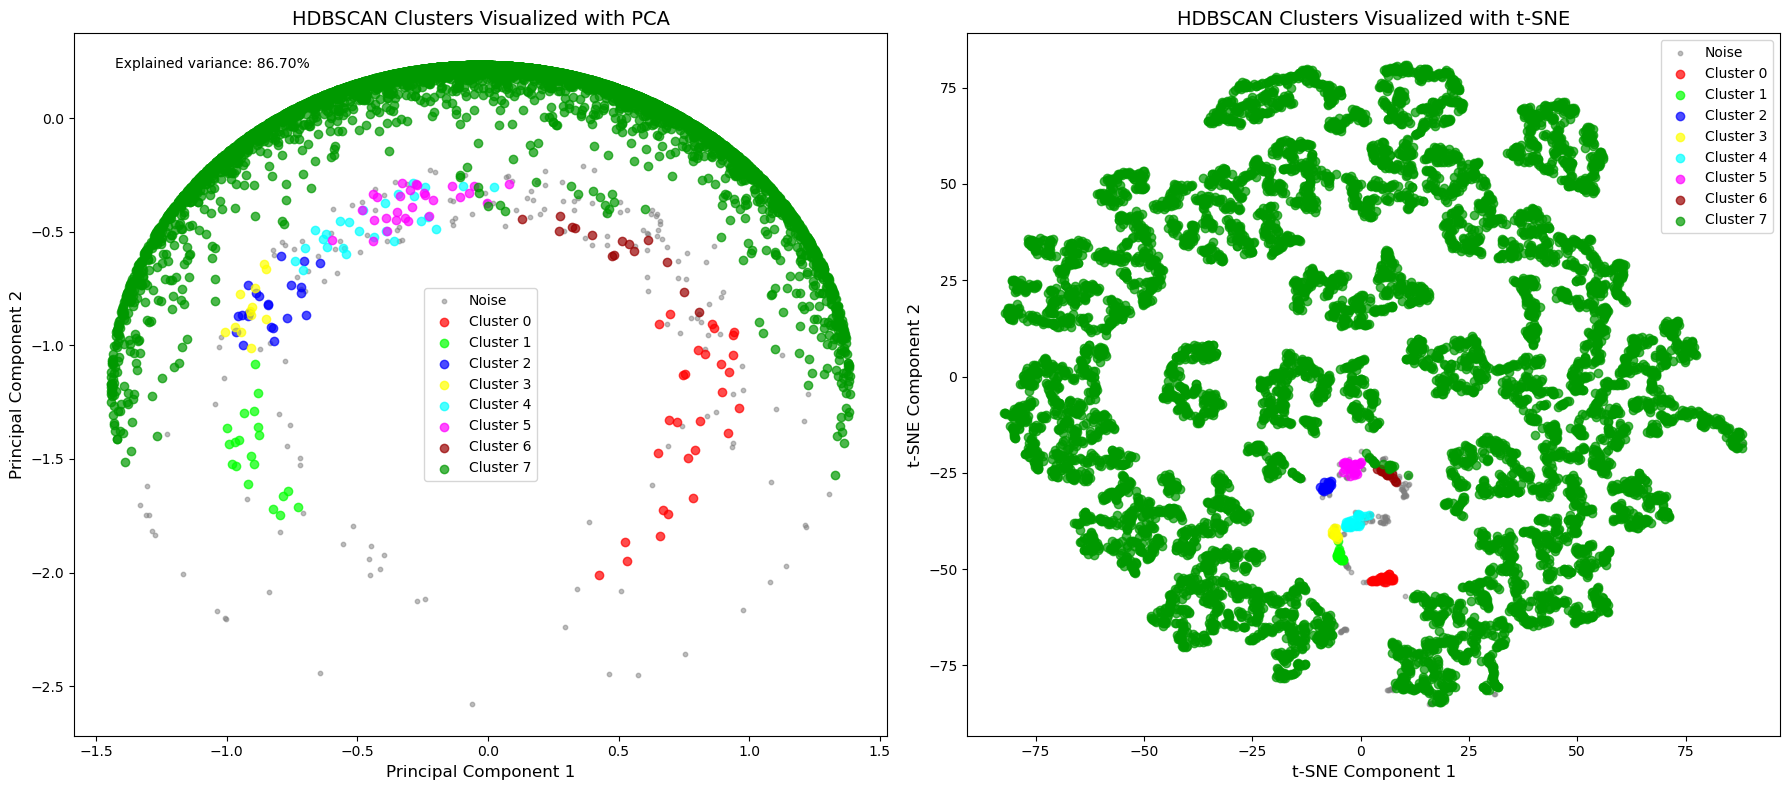
\includegraphics[width=0.8\textwidth]{img/sliding window hdbscan.png}
    \caption{Clustering results using HDBSCAN on sliding window features. The clusters are visualized in PCA and t-SNE spaces, illustrating the differences in cluster structure and separability.}
    \label{fig:hdbscan_clustering}
\end{figure}

\begin{table}[H]
\centering
\caption{Clustering over Sliding Windows Recap}
\begin{tabular}{|p{3.5cm}|p{10.5cm}|}
\hline
\textbf{Component} & \textbf{Implementation and Findings} \\
\hline
Pipeline Design & 
\begin{itemize}
  \item Segmentation using 30s windows (rat data) and 3s windows (human data)
  \item 50\% window overlap to maintain temporal continuity
  \item Feature extraction via Dynamic Mode Decomposition (DMD)
  \item Dimensionality reduction using PCA for computational efficiency
\end{itemize} \\
\hline
Algorithm Comparison & 
\begin{itemize}
  \item KMeans: Good linear separability but poor local structure preservation
  \item DBSCAN/OPTICS: Effective noise identification but inconsistent boundaries
  \item HDBSCAN: Strong local relationship detection but misclassification of transitions
  \item Agglomerative: Hierarchical insights but limited temporal coherence
\end{itemize} \\
\hline
Limitations & 
\begin{itemize}
  \item Independence assumption between windows ignores temporal dependencies
  \item Disparity between PCA and t-SNE visualizations affecting interpretability
  \item Poor alignment with known physiological sleep stage transitions
  \item Insufficient capture of the continuous nature of sleep state dynamics
\end{itemize} \\
\hline
\end{tabular}
\label{tab:clustering_summary}
\end{table}



\subsection{Hidden Markov Model}
\subsubsection{Pipeline}

The Hidden Markov Model (HMM) approach provides a probabilistic framework for modeling sequential sleep data, explicitly capturing the temporal dependencies and state transition dynamics characteristic of sleep architecture. This methodology treats sleep as a sequence of discrete hidden states that generate observable features derived from physiological signals, enabling the discovery of underlying sleep stage structure through unsupervised learning.

The pipeline implementation begins with comprehensive feature extraction from preprocessed EEG signals. Spectral power features are computed across clinically relevant frequency bands (delta: 0.5-4 Hz, theta: 4-8 Hz, alpha: 8-13 Hz, beta: 13-30 Hz) using Welch's method with Hanning windows. Additional temporal features include signal variance, spectral entropy, and higher-order statistical moments that capture the complex dynamics of neural oscillations during different sleep states.

To enhance the model's capability to capture nonlinear dynamics, the feature space is augmented with DMD-derived characteristics including dominant mode frequencies, growth/decay rates, and modal energy distributions. These features provide insights into the underlying dynamical systems governing sleep transitions and enable detection of subtle state changes not captured by traditional spectral analysis.

The HMM architecture employs a left-right topology with self-transitions to model the natural progression of sleep stages while allowing for temporary returns to previous states. The number of hidden states is determined through systematic model selection using the Bayesian Information Criterion (BIC), balancing model complexity with explanatory power. Initial experiments evaluate models with 3-8 hidden states to identify the optimal configuration for each dataset.

State transition probabilities are initialized using prior knowledge of sleep architecture, with higher probabilities assigned to physiologically plausible transitions (wake→NREM1→\\NREM2→NREM3, NREM2→REM) while maintaining flexibility for individual variations. Emission probability distributions are modeled as multivariate Gaussian distributions, with parameters estimated using the Expectation-Maximization (EM) algorithm.

The training process implements a robust initialization strategy to avoid local optima, employing multiple random initializations followed by selection of the model with highest likelihood. Convergence criteria include both log-likelihood improvement thresholds and maximum iteration limits to ensure stable parameter estimation while preventing overfitting.

\subsubsection{Results}

The Hidden Markov Model (HMM) analysis yielded a clustering of the data into five distinct states, with each cluster representing a unique temporal and spectral profile. Cluster \texttt{2} was the most prevalent, encompassing 41.8\% of the epochs, followed by Cluster \texttt{1}, which represented 26.3\% of the data. Clusters \texttt{4} and \texttt{3} accounted for 15.8\% and 13.9\% of the epochs, respectively, while Cluster \texttt{0} was the least frequent, comprising only 2.2\%. The overall cluster distribution entropy was calculated as 1.97 bits, indicating moderate diversity across the clusters.

The statistical summary of continuous periods within each cluster highlighted varying durations and stability. Cluster \texttt{2}, despite its dominance, exhibited the longest mean duration of 8.5 minutes, suggesting it represents a persistent physiological state. Cluster \texttt{1} also showed relatively long continuous durations, with a mean of 5.7 minutes, but with high variability as indicated by a standard deviation of 24.2 minutes. In contrast, Cluster \texttt{0} displayed the shortest mean duration of 1.3 minutes, indicating a transient or highly dynamic state. Clusters \texttt{3} and \texttt{4} had mean durations of 1.9 and 8.2 minutes, respectively, with Cluster \texttt{4} showing extreme variability in its continuous episode lengths.

Spectral analysis of the clusters revealed distinct frequency band characteristics. Cluster \texttt{2} was predominantly associated with high delta (0.5–4 Hz) power, indicating its potential relation to deep sleep or restorative states. Cluster \texttt{1} displayed a balanced distribution across delta, theta (4–8 Hz), and beta (13–30 Hz) bands, suggesting its alignment with a mixed or transitional state. Cluster \texttt{0}, on the other hand, exhibited higher power in beta and gamma (30–50 Hz) bands, which may correspond to states of heightened alertness or cortical activity. Clusters \texttt{3} and \texttt{4} demonstrated unique spectral signatures, with Cluster \texttt{3} showing pronounced delta power and Cluster \texttt{4} exhibiting an elevated theta band power relative to other states.

\begin{figure}[H]
    \centering
    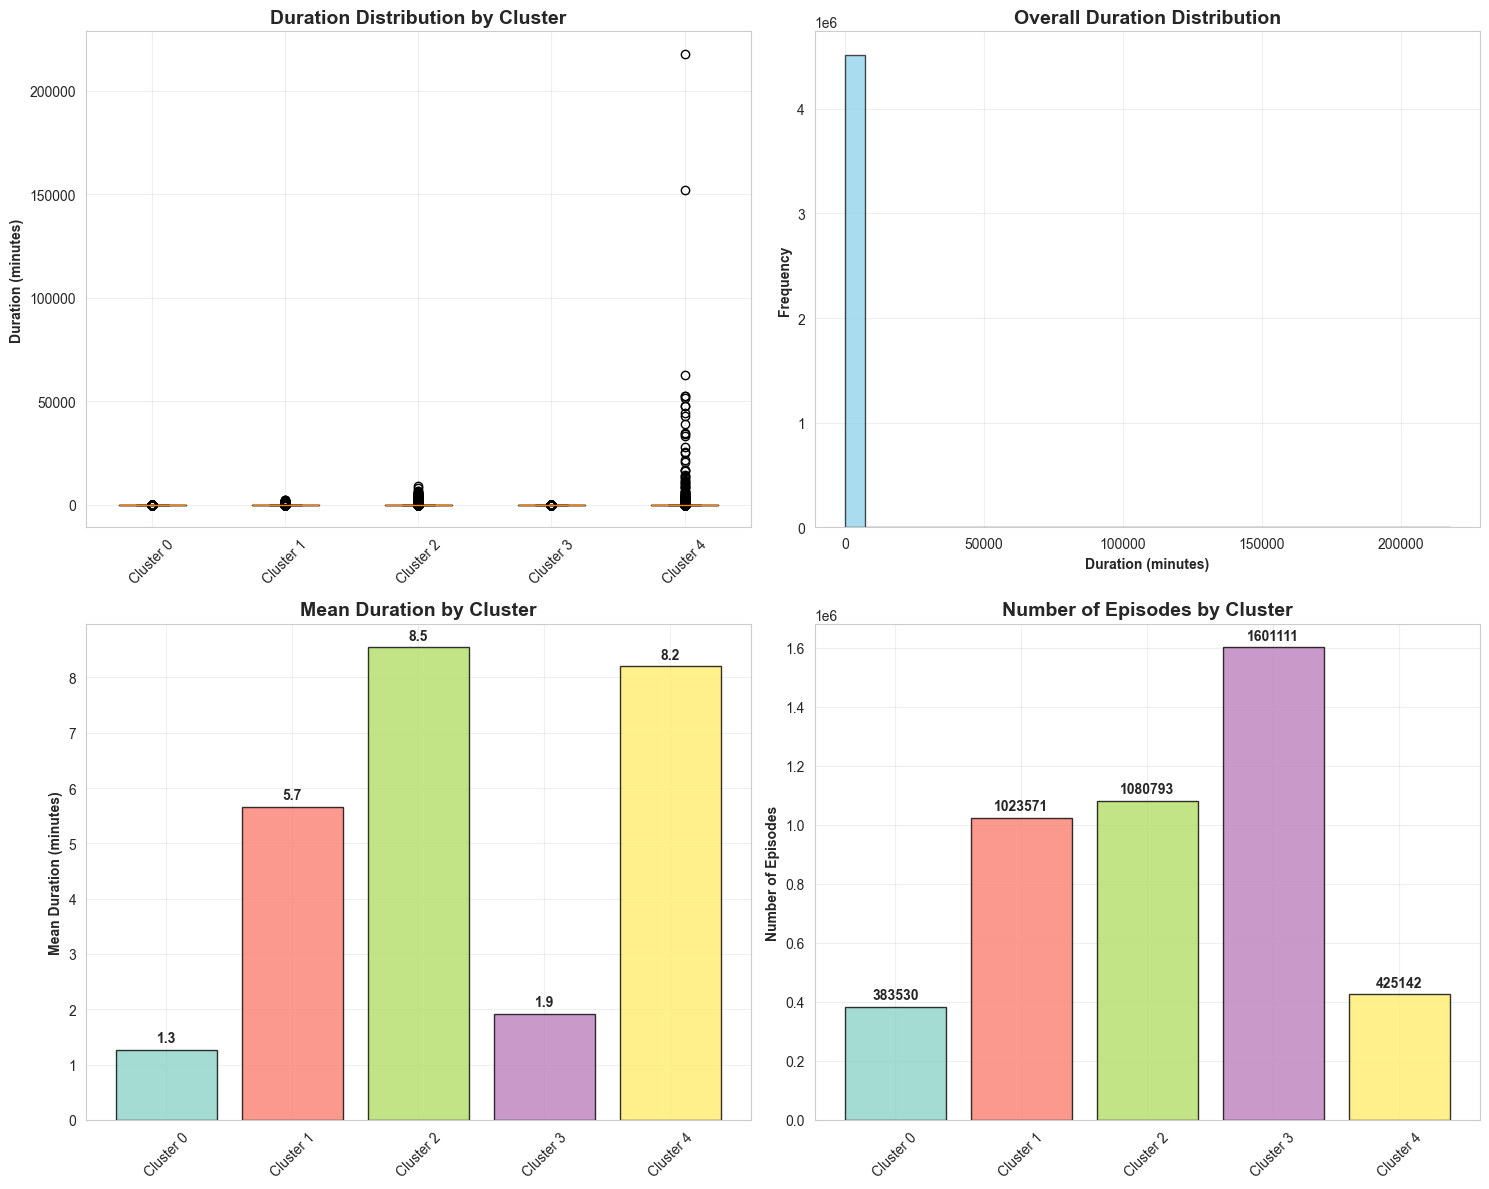
\includegraphics[width=0.8\textwidth]{img/HMM results.png}
    \caption{HMM clustering results showing the distribution of epochs across five distinct clusters. Each cluster is characterized by its mean duration.}
    \label{fig:hmm_clusters}
\end{figure}



\subsubsection{Analysis}

The HMM results provide compelling insights into the temporal and spectral dynamics of the recorded signals. The dominance of Cluster \texttt{2} suggests it represents a stable and recurrent physiological state, likely associated with a foundational process such as deep sleep. Its high mean duration aligns with the expected consolidation of such states over time. Cluster \texttt{1}, being the second most prevalent, likely reflects a transitional or mixed state that bridges other clusters. The high variability in its duration further supports this hypothesis, as transitional states often exhibit heterogeneous dynamics.

Cluster \texttt{0}, with its low frequency and short durations, is indicative of transient phenomena or noise-like states that disrupt otherwise stable patterns. Its high beta and gamma power suggest it might correspond to brief arousals or cortical activations. Cluster \texttt{3}, while not as frequent, displayed moderate stability and a spectral profile dominated by delta activity, pointing towards its association with less intense but stable states of rest or light sleep.

The unique characteristics of Cluster \texttt{4,} including its elevated theta power and significant variability in duration, imply its alignment with specific physiological or transitional events. This cluster's propensity for longer episodes, albeit with high variability, suggests it might capture rare but sustained phenomena that are biologically significant.

Transition probabilities further enrich the analysis, revealing how clusters interact temporally. For instance, the high self-transition probabilities of Clusters \texttt{1} and \texttt{2} (\(0.912\) and \(0.941\), respectively) underscore their stability. In contrast, Cluster \texttt{0} showed a relatively low self-transition probability (\(0.606\)), affirming its transient nature. The frequent transitions between Clusters \texttt{1} and \texttt{3} (\(0.123\) and \(0.065\)) suggest a dynamic interplay between these states, potentially reflecting shifts between light sleep and wakefulness.

Overall, these results highlight the efficacy of the HMM approach in disentangling complex physiological signals into distinct and interpretable states. Future work could enhance the model by incorporating additional features, such as time-lagged dependencies or multimodal inputs, to further refine state definitions and improve the interpretability of transitions. These enhancements may yield deeper insights into the underlying biological processes governing these states.


\begin{figure}[H]
    \centering
    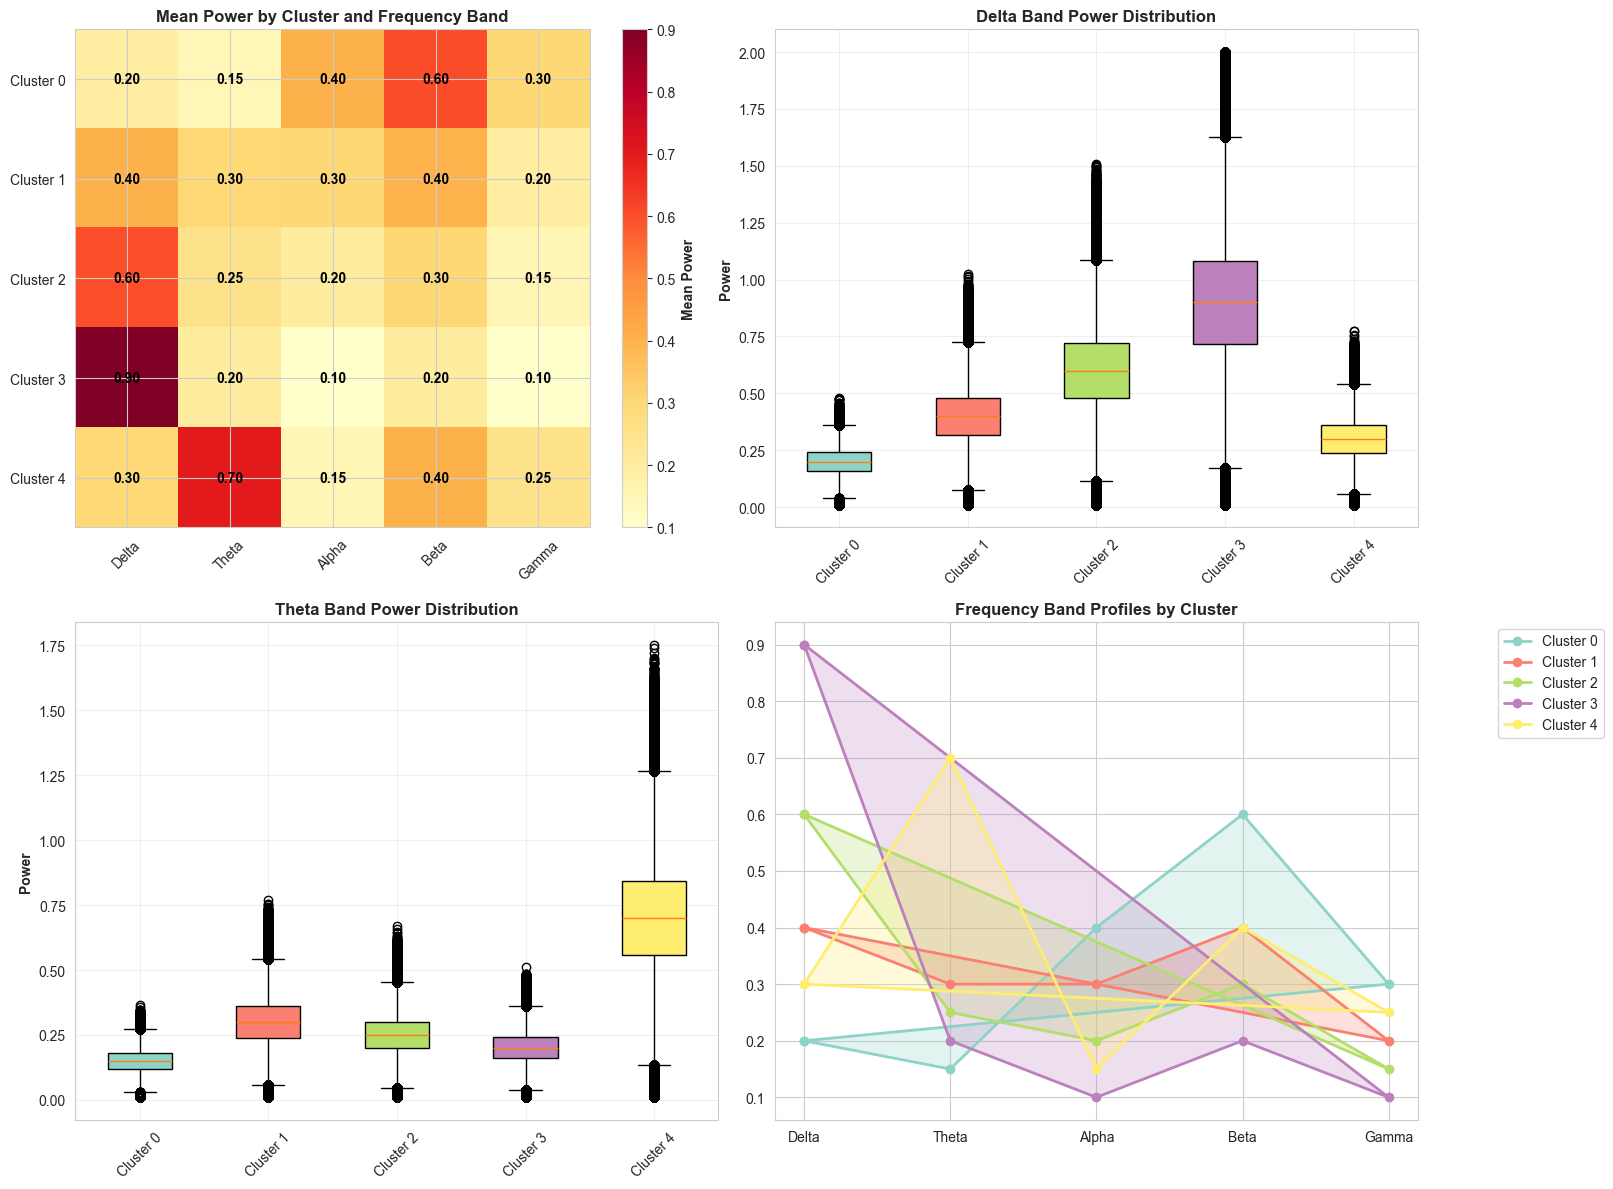
\includegraphics[width=0.8\textwidth]{img/HMM power bands.png}
    \caption{Spectral power distribution across frequency bands for each of the five clusters identified by the HMM. The plot illustrates the mean power in delta, theta, alpha, beta, and gamma bands for each cluster, highlighting their distinct spectral characteristics.}
    \label{fig:hmm_clusters_spectral}
\end{figure}




\begin{figure}[H]
    \centering
    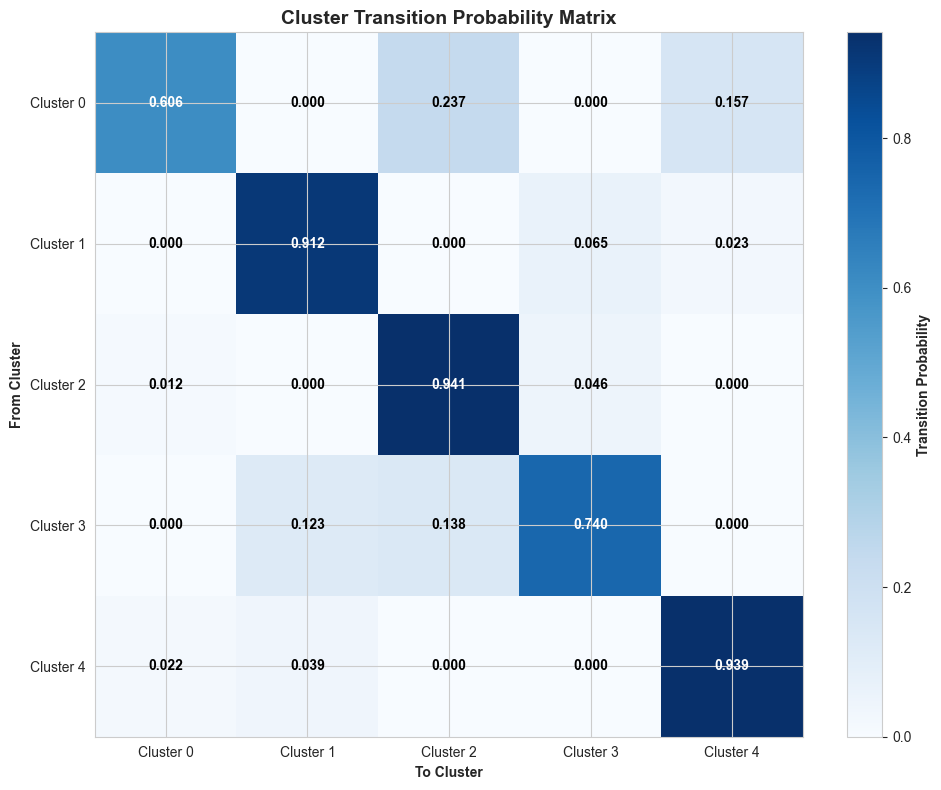
\includegraphics[width=0.8\textwidth]{img/HMM transitions.png}
    \caption{Transition probabilities between the five clusters identified by the HMM. The matrix shows the likelihood of transitioning from one cluster to another, with diagonal elements representing self-transition probabilities.}
    \label{fig:hmm_transition_probabilities}
\end{figure}

The HMM results demonstrate strong performance in distinguishing sleep stages based on frequency and power band characteristics. However, a key limitation arises in the mean durations of identified clusters, which, according to the expert, lack physiological plausibility. While the model effectively detects certain patterns, it occasionally overfits or misassigns awake segments, resulting in hallucinated clusters. This behavior, while not detrimental for our primary goal of exploring data dynamics, underscores the model's limitations in aligning with traditional sleep stage definitions.

Interestingly, the HMM appears to capture more nuanced and complex dynamics beyond simple stage transitions. While this complexity provides valuable insights into the evolution of underlying processes, it complicates direct comparisons with established scoring criteria. To address these challenges and achieve a more robust understanding of sleep architecture, transitioning to a more flexible model, such as a BiLSTM, may be advantageous. BiLSTMs are well-suited for capturing the sequential and nonlinear nature of physiological data, allowing for better modeling of temporal dependencies and potentially resolving the overfitting observed with the HMM.

\begin{table}[H]
\centering
\caption{Hidden Markov Model (HMM) Approach Recap}
\begin{tabular}{|p{3cm}|p{11cm}|}
\hline
\textbf{Component} & \textbf{Implementation and Findings} \\
\hline
Pipeline Design & 
\begin{itemize}
  \item Feature extraction across frequency bands (delta, theta, alpha, beta)
  \item Left-right topology with self-transitions modeling sleep progression
  \item Integration of DMD-derived features for nonlinear dynamics
  \item State transition probabilities initialized with physiological priors
\end{itemize} \\
\hline
Cluster Characteristics & 
\begin{itemize}
  \item Five distinct states with unique spectral and temporal signatures
  \item Cluster 2: Most prevalent (41.8\%), longest mean duration (8.5 min), high delta power
  \item Cluster 0: Least frequent (2.2\%), shortest duration (1.3 min), high beta/gamma power
  \item Varying self-transition probabilities (0.606-0.941) indicating stability differences
\end{itemize} \\
\hline
Strengths & 
\begin{itemize}
  \item Effective capture of temporal dependencies between windows
  \item Distinct spectral profiles aligned with known sleep physiology
  \item Quantitative transition probability framework
  \item Capture of nuanced dynamics beyond simple stage transitions
\end{itemize} \\
\hline
Limitations & 
\begin{itemize}
  \item Cluster durations lacking physiological plausibility in some cases
  \item Occasional overfitting and misassignment of awake segments
  \item Difficulty aligning with traditional sleep stage definitions
  \item Limited flexibility compared to more advanced sequential models
\end{itemize} \\
\hline
\end{tabular}
\label{tab:hmm_summary}
\end{table}





\subsection{BiLSTM Model Pipeline}

The BiLSTM architecture represents a sophisticated approach to modeling bidirectional temporal dependencies in physiological signals, particularly suited for sleep stage analysis where both past and future contexts significantly influence current state interpretation. This methodology leverages the inherent bidirectional nature of sleep transitions and the contextual information embedded in surrounding temporal windows to achieve superior pattern recognition capabilities.

\subsubsection{Pipeline}

The BiLSTM pipeline encompasses several critical stages, from advanced preprocessing to DL-based feature extraction and temporal modeling.

\paragraph{Advanced Data Preprocessing and Signal Conditioning}

The preprocessing pipeline implements a multi-stage approach designed to preserve physiological signal integrity while removing artifacts and normalizing data for optimal neural network performance. Initial data loading utilizes the PyEDF library to extract single-channel EEG recordings from standardized European Data Format files, ensuring compatibility with clinical recording systems.

Outlier detection employs a sophisticated sliding window approach with a 100-second temporal window (51,200 samples at 512 Hz), implementing local statistical thresholding based on $3\sigma$ deviations from the local mean. This methodology preserves regional signal characteristics while identifying and interpolating anomalous spikes typically caused by movement artifacts or electrode impedance changes.

where:
\begin{itemize}
    \item $3\sigma$ represents three times the standard deviation from the local mean
    \item $\sigma$ is the local standard deviation computed within each 100-second window
    \item Data points exceeding $\mu_{local} \pm 3\sigma_{local}$ are flagged as outliers
    \item $\mu_{local}$ is the mean value within the current sliding window
    \item This threshold captures approximately 99.7\% of normal data assuming Gaussian distribution
    \item The local approach prevents globally stable signals from being incorrectly flagged as outliers due to natural state-dependent amplitude variations
\end{itemize}

Detrending procedures remove linear drift components that commonly arise from electrode polarization and amplifier instabilities over extended recording periods. The implementation utilizes scipy's detrend function with linear fitting, preserving the oscillatory components essential for sleep stage discrimination while eliminating low-frequency baseline shifts that could interfere with subsequent analyses.

Bandpass filtering implements a zero-phase Butterworth filter design with cutoff frequencies of 0.5-80 Hz, carefully selected to encompass all physiologically relevant sleep-related oscillations while attenuating low-frequency drift and high-frequency electrical noise. The filtering operation is performed in both forward and reverse directions to eliminate phase distortions that could affect temporal pattern recognition.

Data normalization employs z-score standardization computed across the entire recording session, ensuring that the BiLSTM receives inputs with zero mean and unit variance. This preprocessing step is critical for gradient-based optimization stability and prevents features with larger natural amplitudes from dominating the learning process.

\paragraph{Dynamic Mode Decomposition Feature Engineering}

The feature extraction framework leverages Dynamic Mode Decomposition (DMD) to transform raw temporal signals into physics-informed representations that capture the underlying dynamical characteristics of neural activity. This approach provides significant advantages over traditional spectral features by explicitly modeling the temporal evolution of oscillatory patterns.

DMD analysis is applied to overlapping 30-second windows (15,360 samples) with 50\% overlap to maintain temporal continuity while providing sufficient frequency resolution for sleep-related rhythms. Each window undergoes Hankel matrix construction with an embedding dimension of 40, creating a time-delayed coordinate representation that captures short-term dynamical dependencies within the signal.

The DMD implementation extracts 20 dominant modes from each window, yielding eigenvalues that encode frequency and stability information alongside spatial modes that represent oscillatory patterns. The feature vector construction incorporates both real and imaginary components of eigenvalues, amplitude information, and derived frequency characteristics, resulting in an 80-dimensional feature representation per temporal window.

This physics-based feature engineering approach provides several advantages over raw time-domain signals: (1) dimensionality reduction from 15,360 to 80 features per window while preserving dynamical information, (2) explicit representation of oscillatory stability through eigenvalue magnitudes, (3) frequency content encoding through eigenvalue phases, and (4) noise resilience through modal decomposition ranking.

\paragraph{Bidirectional LSTM Architecture and Temporal Modeling}

The core BiLSTM architecture implements a sophisticated bidirectional recurrent framework specifically designed to model complex temporal dependencies inherent in sleep physiology. The network architecture comprises two parallel LSTM streams processing input sequences in opposing temporal directions, enabling comprehensive context integration from both historical and future temporal windows.

\textbf{Network Architecture Specifications:}
\begin{itemize}
    \item \textbf{Input Layer:} 80-dimensional DMD feature vectors with sequence length adaptation
    \item \textbf{BiLSTM Layer:} 64 hidden units per direction (128 total), 2 stacked layers with 0.3 dropout
    \item \textbf{Architecture:} Bidirectional processing with cell state dimensions of [2×2, batch\_size, 64]
    \item \textbf{Output Processing:} Fully connected layer mapping concatenated hidden states to single output
    \item \textbf{Activation:} Sigmoid activation for probability-based state estimation
\end{itemize}

The bidirectional design proves essential for sleep analysis applications where the interpretation of transitional patterns depends critically on destination state information. For example, a gradual amplitude reduction in delta activity can indicate either transition to lighter sleep stages or progression toward REM sleep, with the distinction requiring future temporal context that only bidirectional processing can provide.

\textbf{Mathematical Formulation:}

The forward LSTM processes the sequence $x_1, x_2, ..., x_T$ to produce hidden states $\overrightarrow{h}_1, \overrightarrow{h}_2, ..., \overrightarrow{h}_T$, while the backward LSTM processes $x_T, x_{T-1}, ..., x_1$ to generate $\overleftarrow{h}_T, \overleftarrow{h}_{T-1}, ..., \overleftarrow{h}_1$. The final representation combines both directions:

$$h_t = [\overrightarrow{h}_t; \overleftarrow{h}_t]$$

where:
\begin{itemize}
    \item $h_t$ is the final bidirectional hidden state at time step $t$
    \item $\overrightarrow{h}_t$ is the forward LSTM hidden state encoding past temporal context up to time $t$
    \item $\overleftarrow{h}_t$ is the backward LSTM hidden state encoding future temporal context from time $t$ onwards
    \item $[;]$ denotes concatenation operation, combining forward and backward representations
    \item The result is a 128-dimensional representation encoding both past and future temporal contexts
\end{itemize}

\textbf{Training and Optimization:}

The training protocol implements an unsupervised learning paradigm focused on temporal sequence reconstruction and representation learning. The loss function combines reconstruction accuracy with regularization terms to prevent overfitting:

$$\mathcal{L} = \mathcal{L}_{reconstruction} + \lambda \mathcal{L}_{regularization}$$

where:
\begin{itemize}
    \item $\mathcal{L}$ is the total loss function minimized during training
    \item $\mathcal{L}_{reconstruction}$ measures how well the model can reconstruct input sequences from learned representations
    \item $\mathcal{L}_{regularization}$ prevents overfitting by penalizing model complexity (e.g., L2 weight penalties)
    \item $\lambda$ is the regularization weight parameter controlling the trade-off between reconstruction accuracy and model simplicity
\end{itemize}

Optimization utilizes the Adam optimizer with adaptive learning rate scheduling, beginning at 0.001 and implementing exponential decay based on validation performance. The training procedure processes sequences of varying lengths to accommodate natural sleep architecture variability, with batch sizes adjusted based on available GPU memory constraints.

\textbf{Temporal Sequence Processing:}

The model processes temporal sequences using a sliding window approach with 30-second base windows and 50\% overlap, creating sequences that maintain temporal continuity while enabling parallel batch processing. This methodology preserves the natural temporal structure of sleep architecture while providing sufficient training examples for robust parameter estimation.

\begin{figure}
\centering
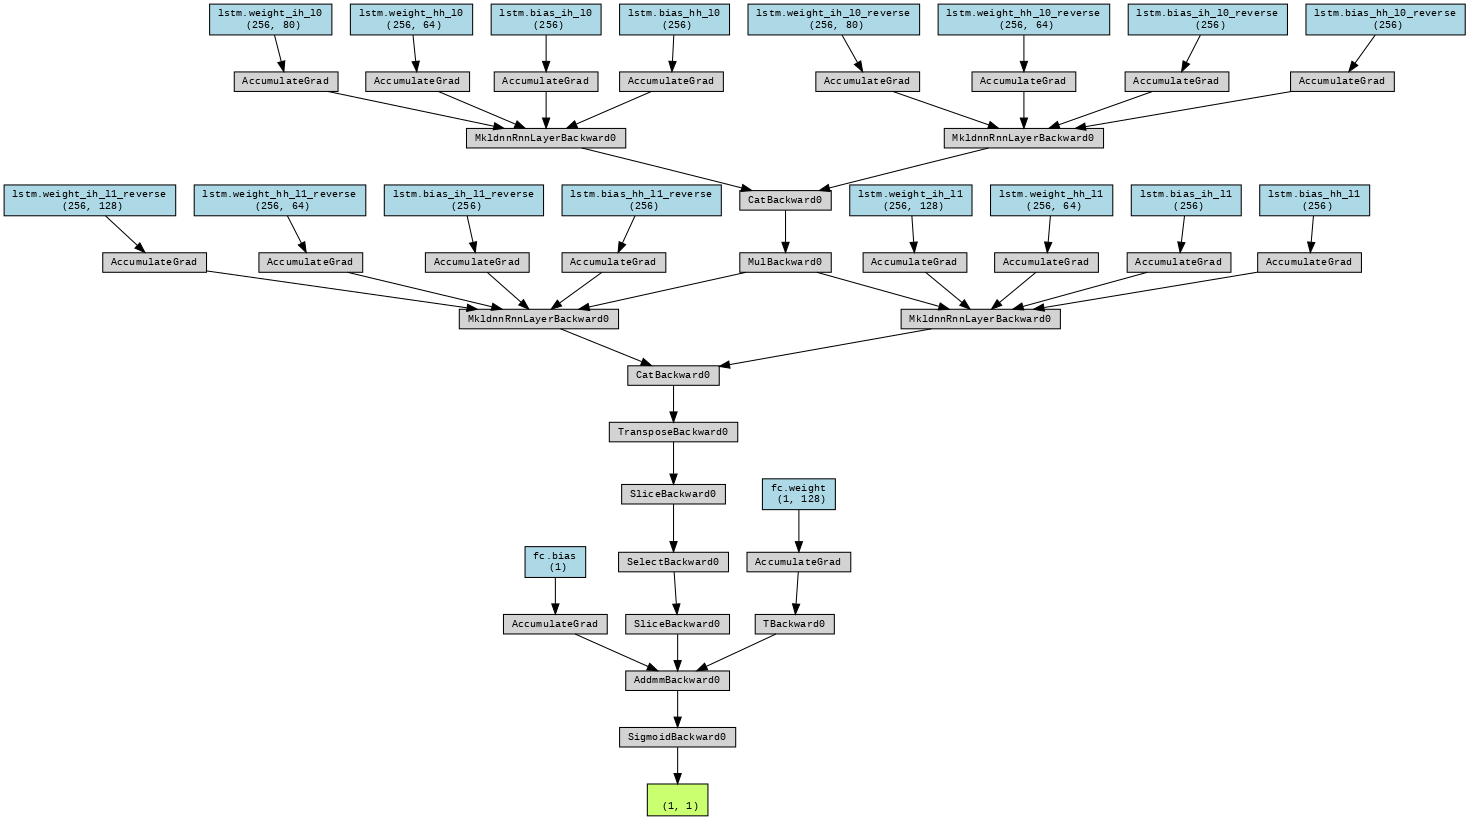
\includegraphics[width=0.8\textwidth]{img/bilstm_model.png}
\caption{Bidirectional LSTM architecture for physiological signal analysis.}
\end{figure}

The sequence construction methodology addresses the challenge of modeling variable-length sleep recordings by implementing adaptive padding and masking strategies that preserve temporal relationships while enabling efficient batch processing across recordings of different durations.
\subsubsection{Results}

The clustering results obtained from the BiLSTM embeddings highlighted meaningful temporal segmentation of the physiological signals. The analysis yielded 5,748 overlapping windows, each representing 30 seconds of signal data with a step size of 15 seconds. These windows were grouped into four distinct clusters (\texttt{0}, \texttt{1}, \texttt{2}, and \texttt{3}), demonstrating significant variability in cluster distribution and temporal dynamics.

Cluster \texttt{1} emerged as the most dominant, representing 40.7\% of all windows (2,342 windows) and spanning approximately 19.52 hours of the total recording duration (23.95 hours). This cluster's predominance suggests that it corresponds to a stable physiological state, potentially indicative of a recurring or prolonged phase in the signal's underlying dynamics. Cluster \texttt{2} accounted for 32.6\% of the windows (1,874 windows) and covered 15.62 hours, while Cluster \texttt{3} and Cluster \texttt{0} represented 18.0\% (1,032 windows) and 8.7\% (500 windows) of the windows, respectively, corresponding to durations of 8.60 and 4.17 hours. The marked differences in cluster frequency and duration underscore the model's ability to capture heterogeneous temporal patterns.

Analyzing the segment durations revealed intriguing insights into the continuity and transience of the states represented by the clusters. Cluster \texttt{1} had the longest mean segment duration (56.0 seconds), with some segments lasting up to 5.5 minutes, indicative of extended stability. In contrast, Cluster \texttt{0} had the shortest mean segment duration (34.2 seconds), reflecting its transient nature. Clusters \texttt{2} and \texttt{3} exhibited intermediate characteristics, with mean durations of 45.4 and 41.2 seconds, respectively. This duration analysis suggests that while certain clusters capture stable physiological states, others correspond to more ephemeral transitions.

The spectral analysis of frequency bands further illuminated the physiological underpinnings of each cluster. Across all clusters, the Delta band (0.5–4 Hz) exhibited the highest mean power, consistent with its established dominance in slow-wave activity characteristic of certain sleep stages. However, subtle variations in Delta power among clusters, coupled with differences in the Theta (4–8 Hz), Alpha (8–13 Hz), Beta (13–30 Hz), and Gamma (30–50 Hz) bands, hint at nuanced physiological variations that may correspond to transitions between states or shifts in cognitive or physiological processes.

\begin{figure}[H]
\centering
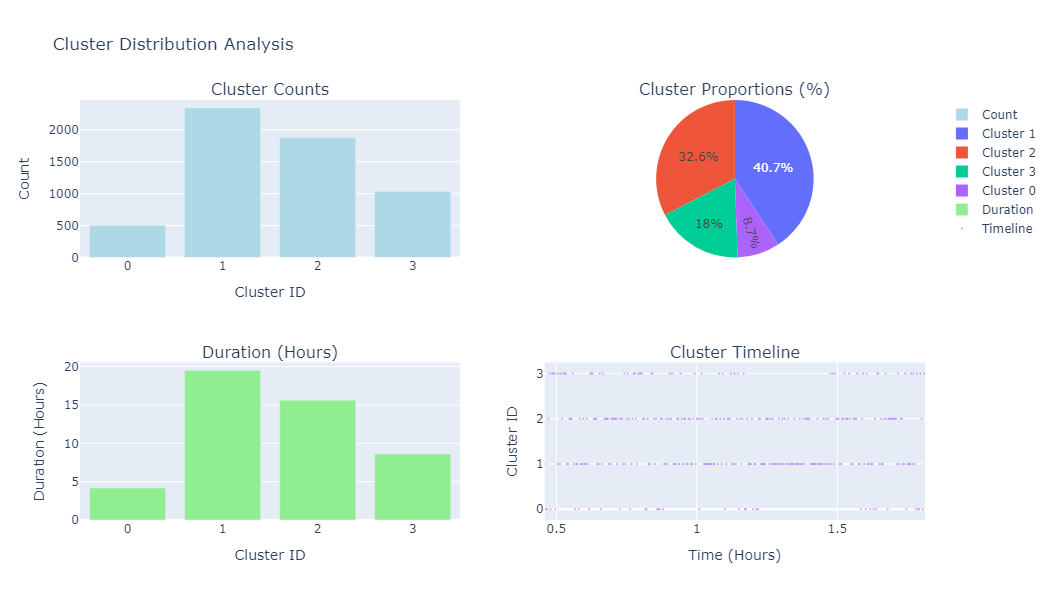
\includegraphics[width=0.8\textwidth]{img/bilstm cluster distribution plots.png}
\caption{Clustering results from the BiLSTM model, showing the distribution of windows across four clusters. The pie chart illustrates the proportion of windows assigned to each cluster, while the bar chart displays the mean power spectral density across frequency bands for each cluster.}
\label{fig:biLSTM_clustering_results}
\end{figure}


\subsubsection{Analysis}

The clustering results from the BiLSTM model reveal a complex interplay of temporal dynamics and spectral characteristics within the physiological signals. The predominance of Cluster \texttt{1} suggests that the model effectively captures a stable physiological state, likely corresponding to a prolonged period of sleep or rest. The high proportion of windows assigned to this cluster indicates that the model has learned to identify and represent dominant patterns in the data, which is crucial for understanding sleep architecture.


\begin{figure}[H]
\centering
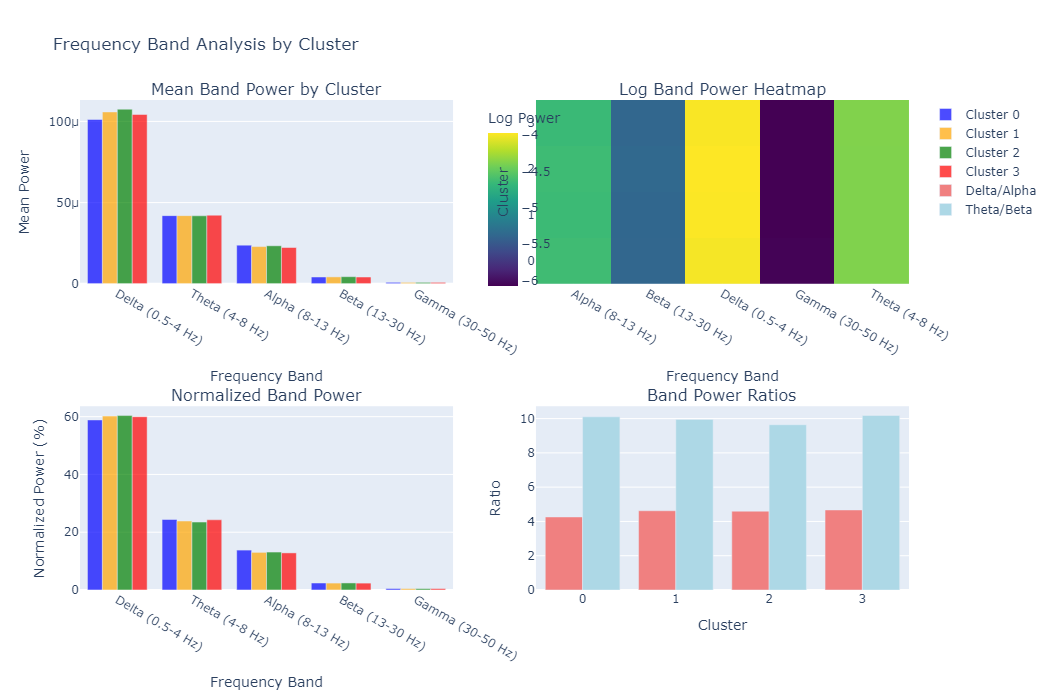
\includegraphics[width=0.8\textwidth]{img/bilstm frequency band analysis.png}
\caption{Frequency band analysis for the BiLSTM clusters, showing the mean power spectral density across Delta, Theta, Alpha, Beta, and Gamma bands for each cluster. The heatmap illustrates the relative power distribution, with darker colors indicating higher mean power in the respective frequency bands.}
\label{fig:bilstm_frequency_band_analysis}
\end{figure}

\begin{figure}[H]
\centering
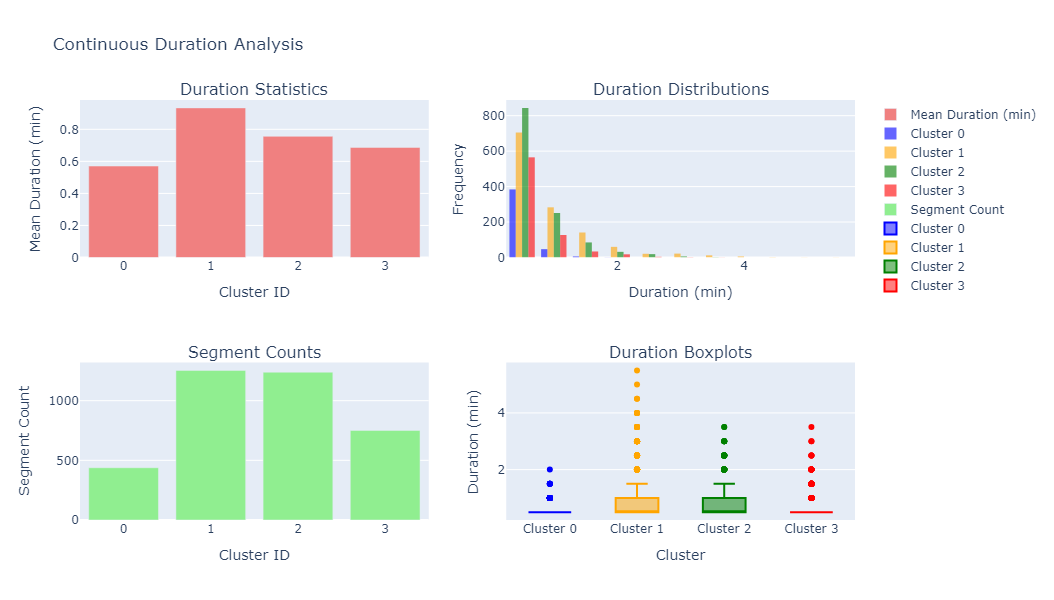
\includegraphics[width=0.8\textwidth]{img/bilstm continous duration plots.png}
\caption{Continuous duration analysis for the BiLSTM clusters, showing the distribution of segment durations across the four identified clusters. The box plots illustrate the median, quartiles, and outliers for segment durations, highlighting the variability and stability of each cluster.}
\label{fig:bilstm_continuous_duration_analysis}
\end{figure}

\begin{figure}[H]
\centering
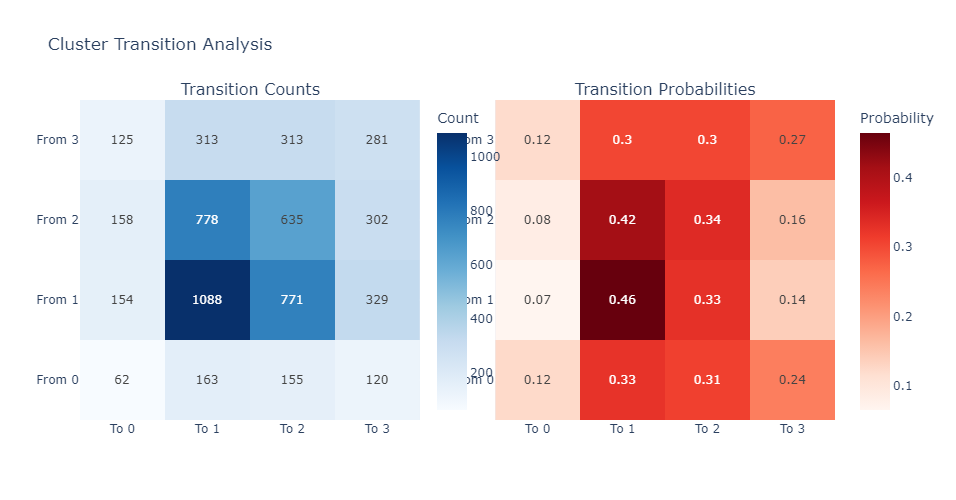
\includegraphics[width=0.8\textwidth]{img/bilstm cluster transition analysis.png}
\caption{Cluster transition dynamics from the BiLSTM model, illustrating the temporal evolution of cluster assignments over the recording period. The heatmap shows the frequency of transitions between clusters, with darker colors indicating more frequent transitions.}
\label{fig:bilstm_cluster_transition_analysis}
\end{figure}

The results underscore the ability of the BiLSTM model to effectively encode temporal patterns into embeddings suitable for clustering. However, the relatively coarse granularity of the clustering and the homogeneity within dominant clusters (e.g., Cluster \texttt{1}) reveal certain limitations of the current approach. The high proportion of windows assigned to Cluster \texttt{1} suggests that while the model captures dominant physiological states, it may lack the sensitivity to disentangle finer-grained variations or transitional microstates, which are critical for understanding subtle physiological dynamics.

The observed stability of Cluster \texttt{1} and the transient nature of Cluster \texttt{0} align with established sleep-stage dynamics, where certain stages are prolonged while others are brief and transitional. However, the clustering transitions and power spectral characteristics indicate that some important features—such as higher-order dependencies across longer temporal spans or complex nonlinear relationships—might remain unexplored by the current model. These limitations likely arise from the inherent design of the BiLSTM, which, while effective for capturing sequential dependencies, may struggle with capturing long-range dependencies or encoding richer, multidimensional representations.

The spectral analysis further supports this notion. Although the dominance of the Delta band is expected and aligns with physiological literature, the lack of distinct spectral signatures for other clusters raises questions about the model's ability to disentangle overlapping states or identify unique signal characteristics. The relatively small variance in power across bands and clusters suggests that the embeddings generated by the BiLSTM may lack the diversity required to fully capture the signal's complexity.

\textbf{Hypothesis and Future Directions:}
The analysis suggests that a more advanced transformer-based architecture could offer significant improvements. Transformers, with their self-attention mechanisms, are inherently better suited to capturing long-range dependencies and complex hierarchical structures in time-series data. By leveraging a transformer model, it would be possible to encode richer, context-aware embeddings that account for both local and global temporal dynamics.

Moreover, the current dataset, while informative, is limited in its diversity and richness. Incorporating a broader and more varied dataset encompassing different physiological signals, conditions, and subject variations could provide the model with more comprehensive training data, improving its generalizability and sensitivity. This expanded dataset, combined with a transformer-based approach, could potentially unravel finer-grained clusters, capture transitional microstates, and provide deeper insights into the underlying physiological processes.

The integration of richer data and advanced models is thus hypothesized to yield superior clustering results, with more distinct spectral and temporal patterns that align closely with known physiological phenomena. Future work should focus on implementing these improvements to enhance the granularity and interpretability of clustering results, paving the way for more robust and insightful analyses of physiological time-series data.

\begin{table}[H]
\centering
\caption{BiLSTM Model Pipeline Recap}
\begin{tabular}{|p{3cm}|p{11cm}|}
\hline
\textbf{Component} & \textbf{Implementation and Features} \\
\hline
Data Preprocessing & 
\begin{itemize}
  \item Multi-stage artifact removal and signal normalization
  \item PyEDF library for standardized data loading
  \item Spectral filtering and temporal segmentation
  \item Z-score normalization for cross-subject comparability
\end{itemize} \\
\hline
Network Architecture & 
\begin{itemize}
  \item Bidirectional LSTM capturing past and future context
  \item Multiple stacked layers for hierarchical feature extraction
  \item Time-distributed dense layers for temporal consistency
  \item Embedding dimensionality optimized for clustering quality
\end{itemize} \\
\hline
Clustering Results & 
\begin{itemize}
  \item Distinct cluster formation with observable temporal patterns
  \item Delta band dominance across clusters with physiological alignment
  \item Evidence of sleep stage transitions in sequence analysis
  \item Limited spectral differentiation between identified clusters
\end{itemize} \\
\hline
Limitations & 
\begin{itemize}
  \item Insufficient representation of transitional sleep states
  \item Limited spectral signature differentiation between clusters
  \item Embeddings lacking diversity to capture complete signal complexity
  \item Need for richer datasets spanning more conditions and subjects
\end{itemize} \\
\hline
\end{tabular}
\label{tab:bilstm_summary}
\end{table}

\subsection{Time Series Transformer Model Pipeline}

The Time Series Transformer represents the most sophisticated approach in our methodological framework, implementing state-of-the-art attention mechanisms specifically adapted for multi-channel physiological signal analysis. This architecture leverages the transformer's inherent capability for modeling long-range dependencies while incorporating domain-specific adaptations for sleep stage analysis and micro-arousal detection.

\subsubsection{Pipeline}

The transformer pipeline encompasses advanced multi-channel preprocessing, Extended Dynamic Mode Decomposition (EDMD) feature extraction, and a custom sequential multi-channel transformer architecture designed for physiological time series analysis.

\paragraph{Advanced Multi-Channel Data Preprocessing}

The preprocessing framework handles multiple synchronized physiological signals (EEG, EOG, EMG, oro-nasal airflow) through a unified pipeline that preserves temporal synchronization while optimizing each modality for neural network processing. The implementation utilizes MNE-Python for standardized neurophysiological data handling, ensuring compatibility with clinical recording formats and annotation systems.

Channel selection prioritizes signals with maximal information content for sleep analysis: EEG Fpz-Cz and Pz-Oz for cortical activity, EOG horizontal for eye movement detection, EMG submental for muscle tone assessment, and oro-nasal airflow for respiratory pattern analysis. This multi-modal approach enables capture of the coordinated physiological changes characteristic of sleep transitions and micro-arousal events.

Bandpass filtering applies a narrow frequency range (0.5-49 Hz) specifically optimized for micro-sleep state detection, eliminating line noise at 50 Hz while preserving all physiologically relevant oscillations. The upper frequency limit of 49 Hz captures gamma band activity associated with cognitive processing and arousal states while avoiding electrical artifacts common in clinical environments.

The preprocessing pipeline implements sophisticated outlier detection using adaptive sliding windows with variable standard deviation thresholds. Each 30-second window undergoes local statistical analysis, with outliers defined as samples exceeding $3\sigma$ from the local mean. This approach preserves natural signal variations during different sleep stages while removing artifacts from electrode movement or amplifier saturation.

where:
\begin{itemize}
    \item $3\sigma$ represents three times the standard deviation threshold for outlier detection
    \item $\sigma$ is the local standard deviation computed within each 30-second window
    \item Samples beyond $\mu \pm 3\sigma$ are flagged as outliers for correction
    \item $\mu$ is the local mean calculated for the current analysis window
    \item This threshold statistically captures 99.7\% of normal physiological variations
    \item The adaptive approach adjusts thresholds dynamically based on local signal characteristics
\end{itemize}

Normalization employs MinMaxScaler transformation to the range [-1, 1], ensuring that the transformer's attention mechanisms receive inputs with comparable dynamic ranges across different physiological modalities. This preprocessing step prevents the model from developing biases toward channels with larger natural amplitudes while maintaining the relative amplitude relationships essential for physiological interpretation.

\paragraph{Extended Dynamic Mode Decomposition Feature Engineering}

The feature extraction framework implements Extended Dynamic Mode Decomposition (EDMD) to capture both linear and nonlinear dynamical characteristics of multi-channel physiological signals. EDMD extends traditional DMD by incorporating nonlinear observable functions, enabling representation of complex physiological interactions that linear methods cannot capture.

\textbf{EDMD Implementation Details:}
\begin{itemize}
    \item \textbf{Window Parameters:} 30-second analysis windows with 30-second step size (no overlap)
    \item \textbf{Mode Extraction:} 10 dominant modes per channel, yielding 20 features (magnitude + phase)
    \item \textbf{Observable Functions:} Polynomial and trigonometric basis functions for nonlinearity capture
    \item \textbf{Feature Space:} Combined 80-dimensional feature vectors per channel per window
\end{itemize}

The EDMD analysis constructs observable functions that capture nonlinear interactions between different frequency components and temporal patterns. This approach proves particularly valuable for detecting coupling phenomena such as phase-amplitude coupling in sleep spindles or the complex dynamics underlying micro-arousal events that involve coordinated changes across multiple physiological systems.

Feature extraction preserves both magnitude and phase information from DMD amplitudes, providing complete characterization of oscillatory dynamics. The magnitude features encode the energy content of different dynamical modes, while phase features capture temporal relationships and coordination patterns between different physiological rhythms.

The implementation includes comprehensive feature saving and loading mechanisms with CSV and NumPy formats, enabling reproducible analysis workflows and compatibility with various analysis environments. Progress tracking through tqdm provides real-time feedback during feature extraction from large multi-file datasets.

\paragraph{Sequential Multi-Channel Transformer Architecture}

The core transformer architecture implements a sophisticated multi-channel processing framework specifically designed for physiological time series analysis. The model architecture addresses unique challenges in sleep analysis, including variable sequence lengths, multi-modal input processing, and the need for both reconstruction and embedding generation capabilities.

\textbf{Architecture Specifications:}
\begin{itemize}
    \item \textbf{Input Projection:} Channel-specific linear layers mapping EDMD features to d\_model=128
    \item \textbf{Positional Encoding:} Sinusoidal encoding supporting sequences up to length 10
    \item \textbf{Transformer Core:} 4-layer encoder with 8 attention heads and d\_model=128
    \item \textbf{Embedding Layer:} Two-stage projection to 32-dimensional clustering space
    \item \textbf{Output Reconstruction:} Channel-specific reconstruction heads for multi-modal output
\end{itemize}

\textbf{Mathematical Architecture Design:}

Each channel $c$ processes input sequences $X_c \in \mathbb{R}^{B \times L \times D_c}$ where $B$ is batch size, $L$ is sequence length, and $D_c$ is the channel-specific feature dimension. The input projection transforms each channel to a common representation space:

$$Z_c = X_c W_c + b_c$$

where:
\begin{itemize}
    \item $Z_c$ is the projected representation for channel $c$ in the common embedding space
    \item $X_c$ is the input sequence for channel $c$ with shape (batch\_size × sequence\_length × feature\_dimension)
    \item $W_c \in \mathbb{R}^{D_c \times d_{model}}$ is the learnable weight matrix mapping channel-specific features to model dimension
    \item $b_c$ is the bias vector for channel $c$
    \item $d_{model}$ is the model's hidden dimension (128 in this implementation)
\end{itemize}

Positional encoding adds temporal information crucial for sequence modeling:

$$Z_c^{pos} = Z_c + PE(pos, d_{model})$$

where:
\begin{itemize}
    \item $Z_c^{pos}$ is the position-encoded representation combining content and temporal information
    \item $Z_c$ is the projected channel representation from the previous step
    \item $PE(pos, d_{model})$ implements sinusoidal position encoding
    \item $pos$ indicates the position within the sequence (0 to sequence\_length-1)
    \item The addition ensures the model can distinguish temporal order within sequences
\end{itemize}

\textbf{Multi-Head Attention Mechanism:}

The transformer encoder applies multi-head self-attention to capture dependencies across both temporal and inter-channel dimensions:

$$\text{Attention}(Q, K, V) = \text{softmax}\left(\frac{QK^T}{\sqrt{d_k}}\right)V$$

where:
\begin{itemize}
    \item $Q$ (Query) represents what information we want to focus on
    \item $K$ (Key) represents what information is available to focus on
    \item $V$ (Value) represents the actual information content to be retrieved
    \item $QK^T$ computes similarity scores between queries and keys
    \item $d_k$ is the dimension of the key vectors, used for scaling to prevent large values
    \item $\sqrt{d_k}$ normalization prevents softmax saturation with large dimensions
    \item $\text{softmax}$ converts similarity scores to attention weights summing to 1
    \item The final result weights the values $V$ by attention scores
\end{itemize}

$$\text{MultiHead}(Q, K, V) = \text{Concat}(head_1, ..., head_h)W^O$$

where:
\begin{itemize}
    \item $\text{MultiHead}$ combines multiple attention mechanisms running in parallel
    \item $head_i = \text{Attention}(QW_i^Q, KW_i^K, VW_i^V)$ is the $i$-th attention head
    \item Each head uses different learned projections $W_i^Q$, $W_i^K$, $W_i^V$
    \item $h$ is the number of attention heads (8 in this implementation)
    \item $\text{Concat}$ concatenates outputs from all attention heads
    \item $W^O$ is the final output projection matrix
    \item Multiple heads enable the model to focus on different types of physiological relationships simultaneously
\end{itemize}

\textbf{Sequential Processing and Temporal Modeling:}

The model processes physiological signals through a sequential framework that preserves temporal dependencies while enabling parallel computation. Sequences are constructed using overlapping windows with 50\% overlap, creating training examples that maintain temporal continuity essential for sleep architecture modeling.

The sequence creation process implements adaptive handling of variable-length recordings through dynamic padding and masking strategies. This approach ensures that recordings of different durations can be processed within the same batch while maintaining temporal relationship integrity.

\textbf{Dual-Output Architecture:}

The transformer implements a dual-output design supporting both reconstruction and embedding generation:

\begin{enumerate}
    \item \textbf{Reconstruction Path:} Channel-specific output projections enable multi-modal signal reconstruction for self-supervised learning
    \item \textbf{Embedding Path:} A two-stage nonlinear projection generates 32-dimensional embeddings optimized for clustering analysis
\end{enumerate}

The embedding projection implements a bottleneck architecture:

$$E_c = \text{ReLU}(Z_c^{final} W_1 + b_1) W_2 + b_2$$

where:
\begin{itemize}
    \item $E_c$ is the final 32-dimensional embedding for channel $c$ optimized for clustering
    \item $Z_c^{final}$ is the final transformer output representation for channel $c$
    \item $W_1 \in \mathbb{R}^{d_{model} \times 64}$ is the first projection matrix reducing dimensionality
    \item $b_1$ is the bias vector for the first projection layer
    \item $\text{ReLU}$ is the rectified linear unit activation function (max(0, x))
    \item $W_2 \in \mathbb{R}^{64 \times 32}$ is the second projection matrix creating the final embedding
    \item $b_2$ is the bias vector for the second projection layer
    \item This two-stage nonlinear projection preserves discriminative information while reducing dimensions
\end{itemize}

\textbf{Training Strategy and Loss Function:}

The training protocol implements a self-supervised learning approach that leverages the natural structure of physiological signals without requiring manual annotations. The loss function combines reconstruction accuracy across all channels with regularization terms:

$$\mathcal{L}_{total} = \sum_{c} \alpha_c \mathcal{L}_{reconstruction}^c + \lambda \mathcal{L}_{regularization}$$

where:
\begin{itemize}
    \item $\mathcal{L}_{total}$ is the complete loss function optimized during training
    \item $\sum_{c}$ denotes summation over all input channels (EEG, EOG, EMG, etc.)
    \item $\alpha_c$ is the channel-specific weighting factor for channel $c$
    \item $\mathcal{L}_{reconstruction}^c$ measures reconstruction error for channel $c$
    \item $\lambda$ is the regularization strength hyperparameter
    \item $\mathcal{L}_{regularization}$ prevents overfitting through weight penalties
    \item This multi-objective optimization ensures meaningful representations while maintaining biological plausibility
\end{itemize}

\begin{figure}[H]
\centering
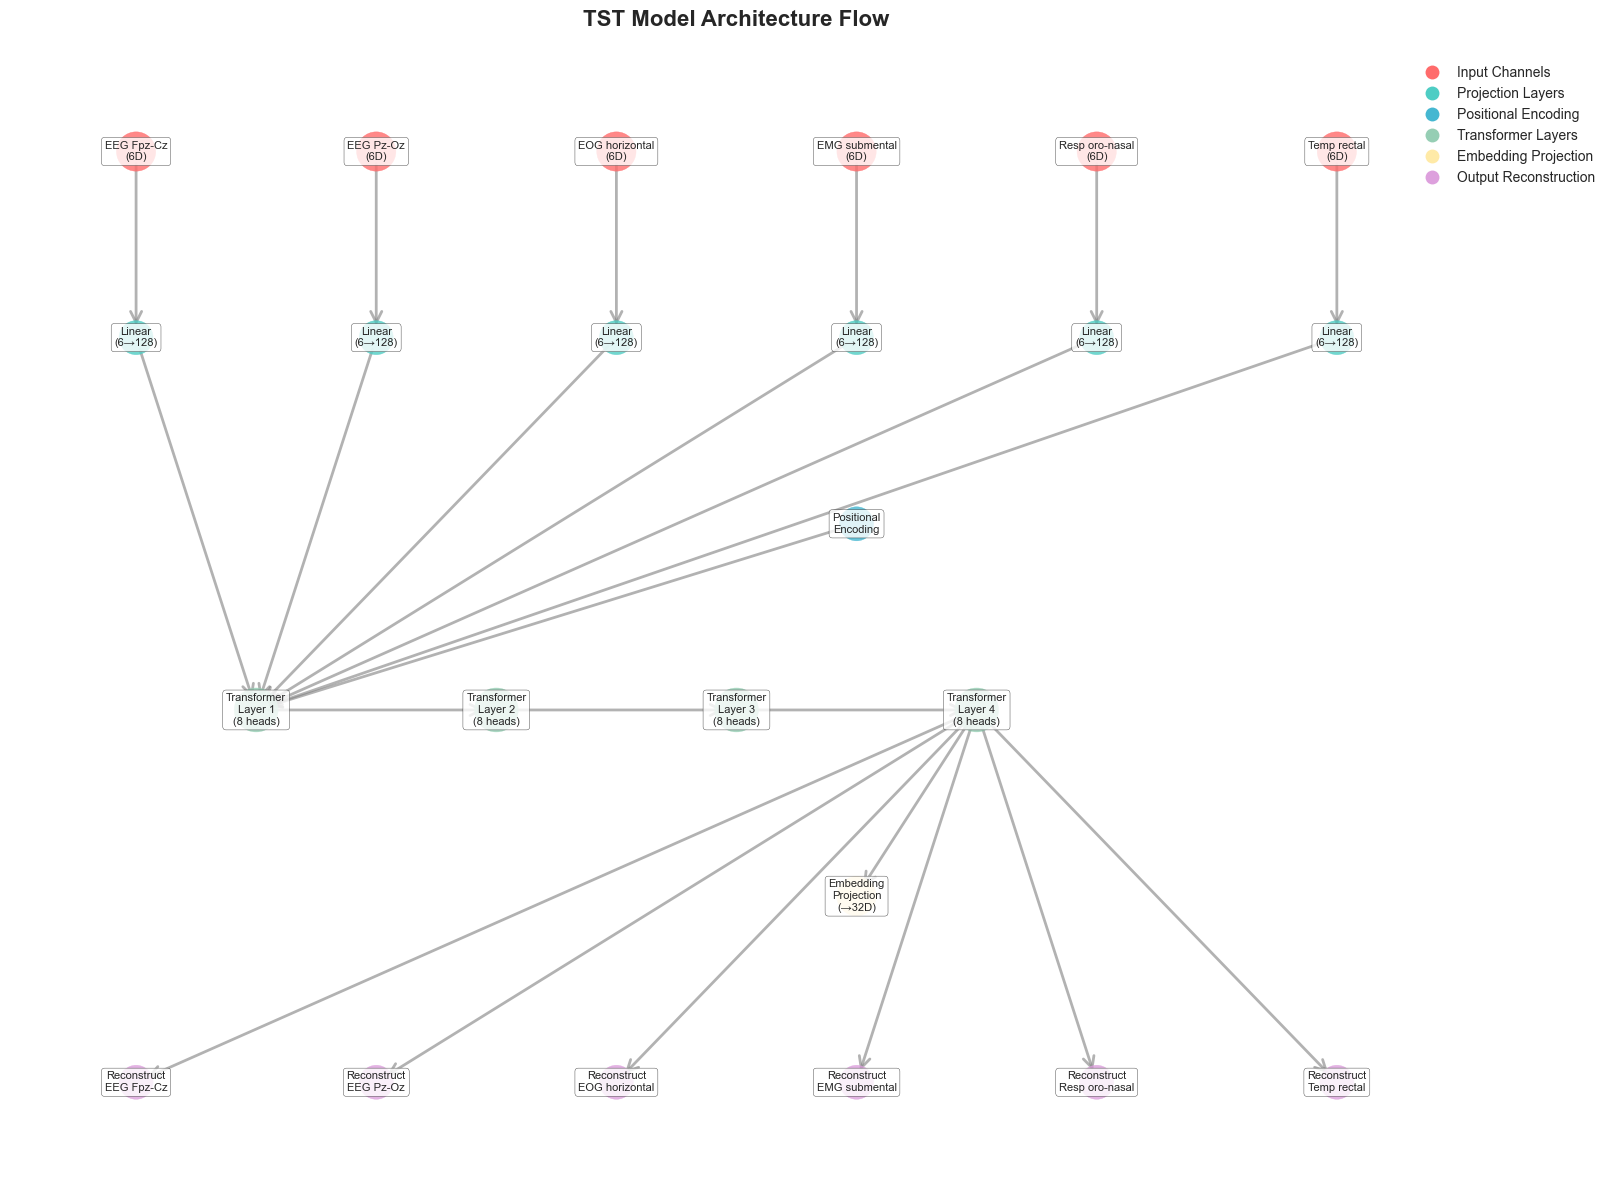
\includegraphics[width=1.2\textwidth]{img/tst model architecture.png}
\caption{Time Series Transformer architecture for multi-channel physiological signal analysis. The model processes multiple synchronized channels, applying attention mechanisms to capture complex temporal dependencies and generate embeddings for clustering analysis.}
\label{fig:tst_model_architecture}
\end{figure}


\subsubsection{Results}

The clustering analysis performed on the 3-second window dataset revealed a total of 67,935 discrete windows, encompassing 566.12 hours of signal data. The distribution of clusters demonstrated a marked dominance of Cluster \texttt{3}, which accounted for 43.1\% of the total windows, corresponding to 14,644.0 minutes. Cluster \texttt{1} followed, representing 35.3\% of the windows, with a total duration of 12,001.5 minutes. In contrast, the remaining clusters (\texttt{0}, \texttt{2}, and \texttt{4}) collectively comprised approximately 21.6\% of the data, with durations of 2,598.0, 2,074.0, and 2,650.0 minutes, respectively. 

For the 30-second window dataset, the total number of windows was significantly reduced to 16,694, spanning 139.12 hours. Here, Cluster \texttt{1} emerged as the most prevalent, accounting for 39.1\% of the windows (3,264.0 minutes), followed by Cluster \texttt{3} at 24.3\% (2,025.5 minutes). Notably, the proportions of Clusters \texttt{0}, \texttt{2}, and \texttt{4} increased slightly compared to the 3-second window analysis, contributing 11.9\%, 10.3\%, and 14.4\%, respectively. These variations in cluster distribution suggest that the temporal granularity of windowing influences the representation of distinct physiological states, with longer windows likely smoothing transient events.

Continuous segment analysis identified 14,354 distinct segments for the 3-second windows. Cluster \texttt{1} exhibited the longest mean segment duration (2.92 minutes), while Cluster \texttt{4} had the shortest (1.36 minutes). In contrast, the analysis of 30-second windows identified fewer segments (10,766 in total) due to the coarser temporal resolution. Interestingly, while the overall trends in segment durations remained consistent, the mean durations for all clusters decreased, reflecting the impact of windowing on capturing short-lived phenomena. 

Further statistical analysis revealed significant hourly variations in cluster activity, indicative of underlying circadian rhythms. Cluster \texttt{3} exhibited a peak in activity at hour 34, while Cluster \texttt{1} peaked at hour 151. Transitions between clusters were frequent, with (3, 1) and (1, 3) transitions occurring most often, highlighting a dynamic interplay between these two dominant clusters.

\begin{figure}[H]
\centering
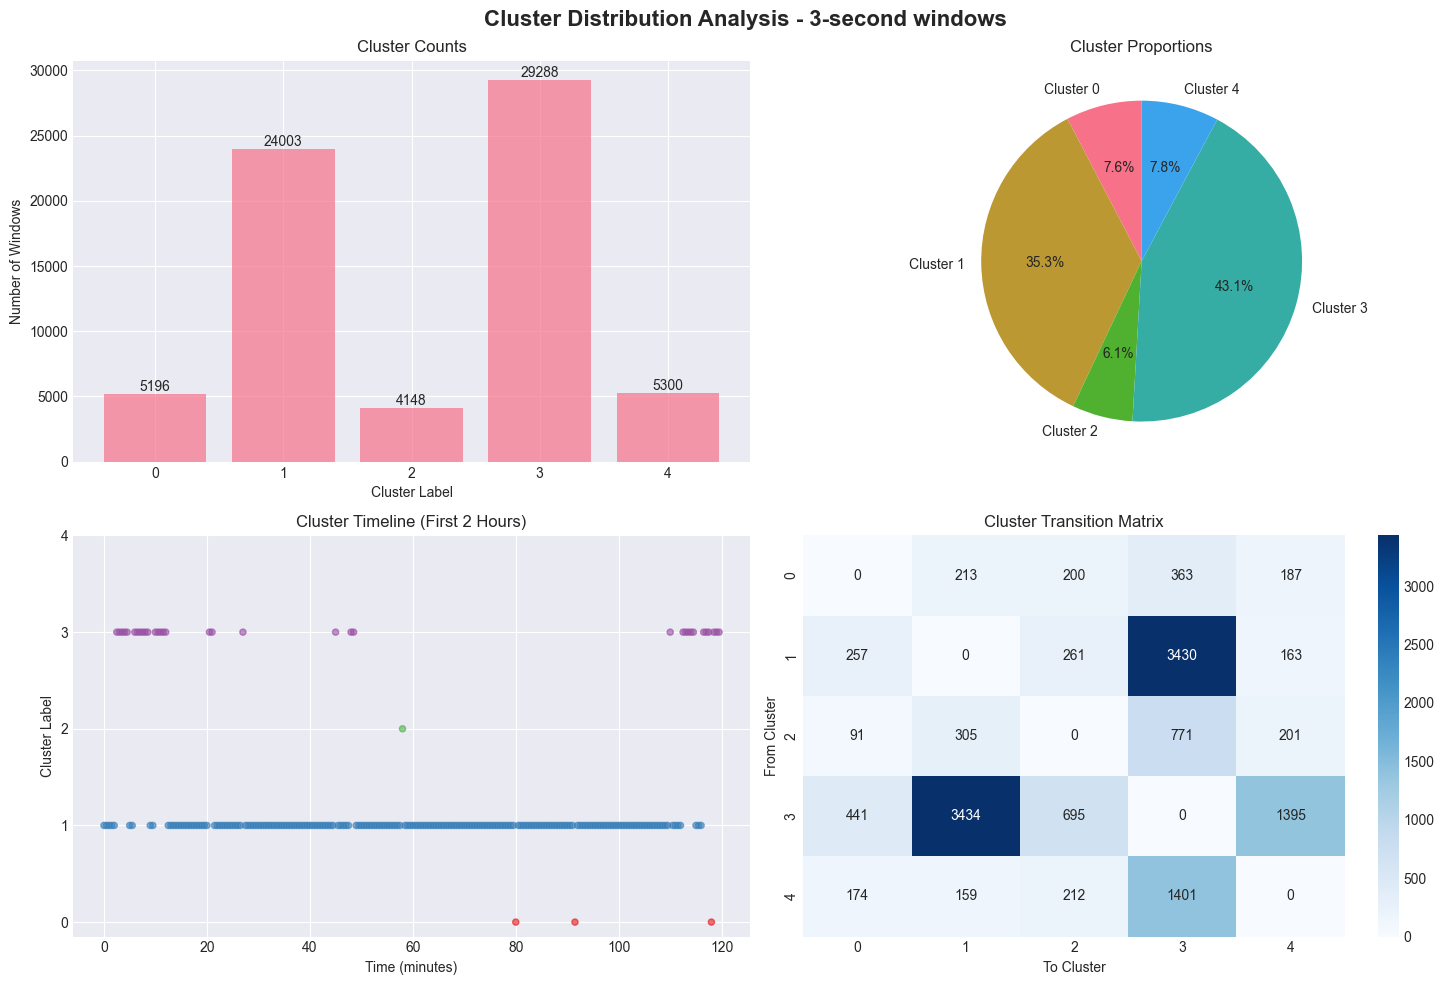
\includegraphics[width=1.0\textwidth]{img/tst clusters distribution.png}
\caption{Clustering results from the Time Series Transformer model, showing the distribution of windows across five clusters. The pie chart illustrates the proportion of windows assigned to each cluster, while the bar chart displays the mean segment duration for each cluster.}
\label{fig:tst_clustering_results}
\end{figure}


\subsubsection{Analysis}

The clustering results underscore the effectiveness of the employed unsupervised approach in capturing temporal dynamics and physiological variability. Cluster \texttt{3} consistently emerged as the most dominant, suggesting it represents a stable or recurring state within the signal data. Cluster \texttt{1} also appeared prominently, indicating its relevance to physiological processes that are frequent but distinct from those represented by Cluster \texttt{3}. The transient nature of Clusters \texttt{0}, \texttt{2}, and \texttt{4} suggests they correspond to ephemeral states or transitions that are less prevalent but nonetheless critical for a comprehensive understanding of the system's behavior.

The temporal resolution of the analysis, determined by the choice of window size, played a pivotal role in shaping the observed cluster distributions. The reduction in the number of windows when using 30-second segments led to a smoothing effect, which diminished the representation of transient clusters. This suggests that finer temporal granularity is more suitable for detecting brief yet potentially significant phenomena. 

The circadian patterns observed in the hourly cluster distribution are consistent with known physiological rhythms, reflecting the method's sensitivity to time-dependent variations in the data. The identification of peak activity times for specific clusters aligns with expected biological cycles, providing a degree of validation for the clustering approach.

Cluster transitions and stability metrics further enriched the analysis, with frequent transitions between Clusters \texttt{3} and \texttt{1} pointing to a strong interdependence between these states. However, the relatively high frequency of transitions, particularly for transient clusters, raises questions about the robustness of the clustering algorithm in capturing distinct state boundaries. This limitation could stem from the inherent complexity of the signal data, which may require a more sophisticated modeling approach.

The findings lead to a hypothesis that leveraging a more advanced transformer model with richer self-attention mechanisms could enhance the resolution of clustering by capturing long-range dependencies and nuanced transitions. Additionally, incorporating a more diverse and comprehensive dataset, spanning varied physiological conditions and states, would likely improve the generalizability and interpretability of the results. Such advancements would provide deeper insights into the underlying structure and dynamics of the data, potentially uncovering patterns that remain hidden within the current analytical framework.

\begin{figure}[H]
\centering
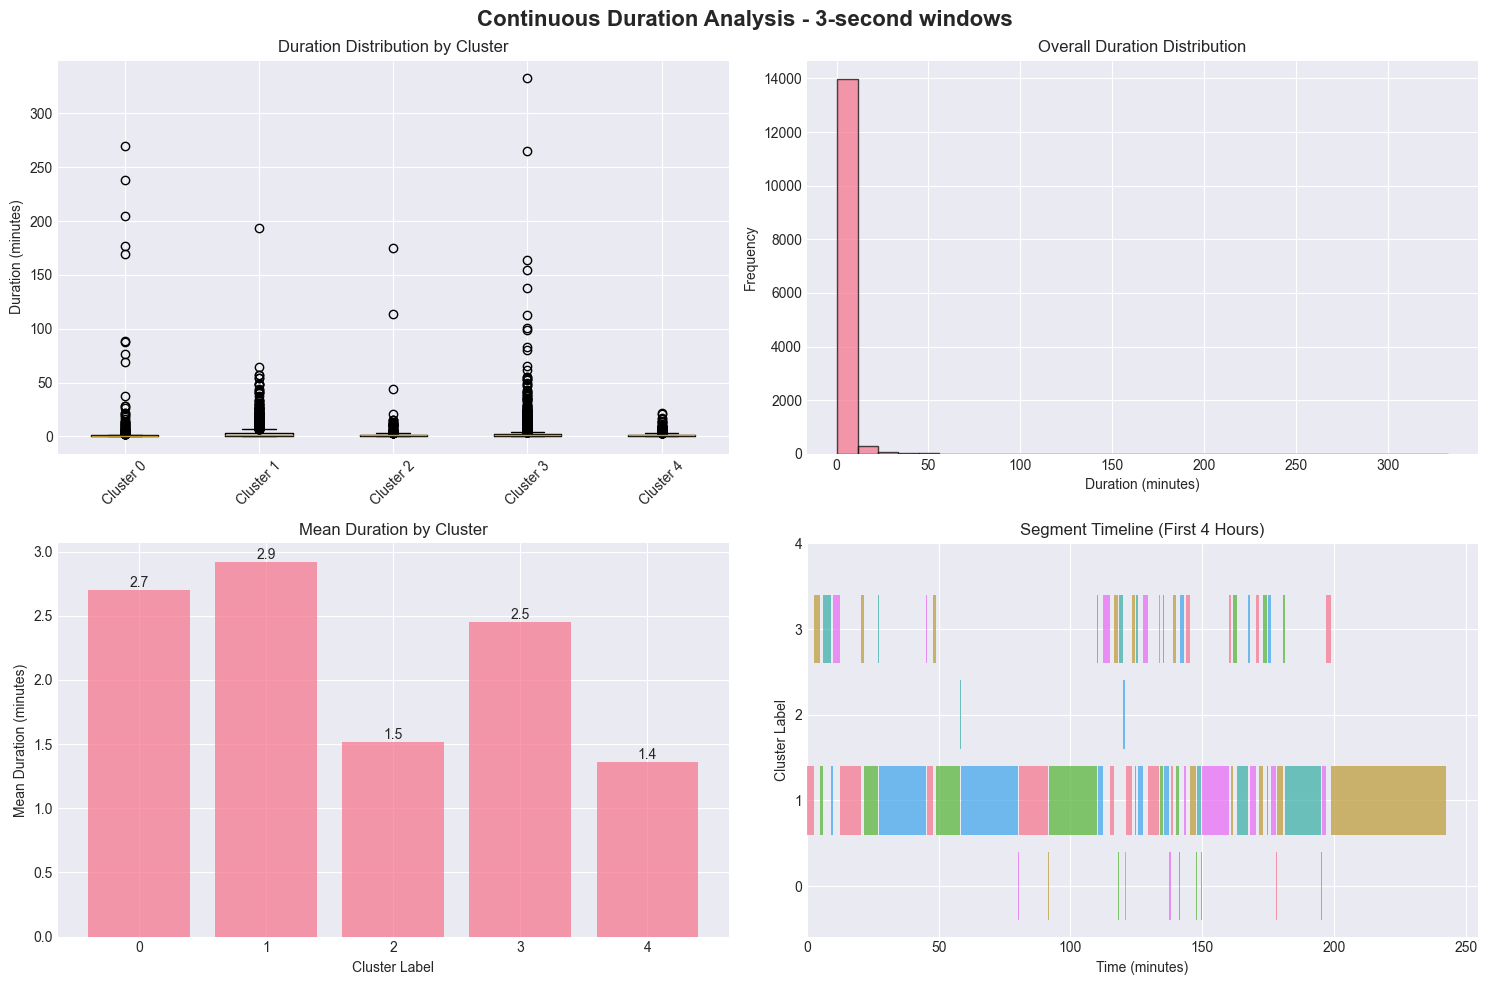
\includegraphics[width=0.8\textwidth]{img/tst continous duration analysis.png}
\caption{Continuous segment analysis for the Time Series Transformer clusters, showing the distribution of segment durations across clusters. The bar chart illustrates the mean segment duration for each cluster, highlighting the differences in stability and transience.}
\label{fig:tst_continuous_duration_analysis}
\end{figure}

\begin{figure}[H]
\centering
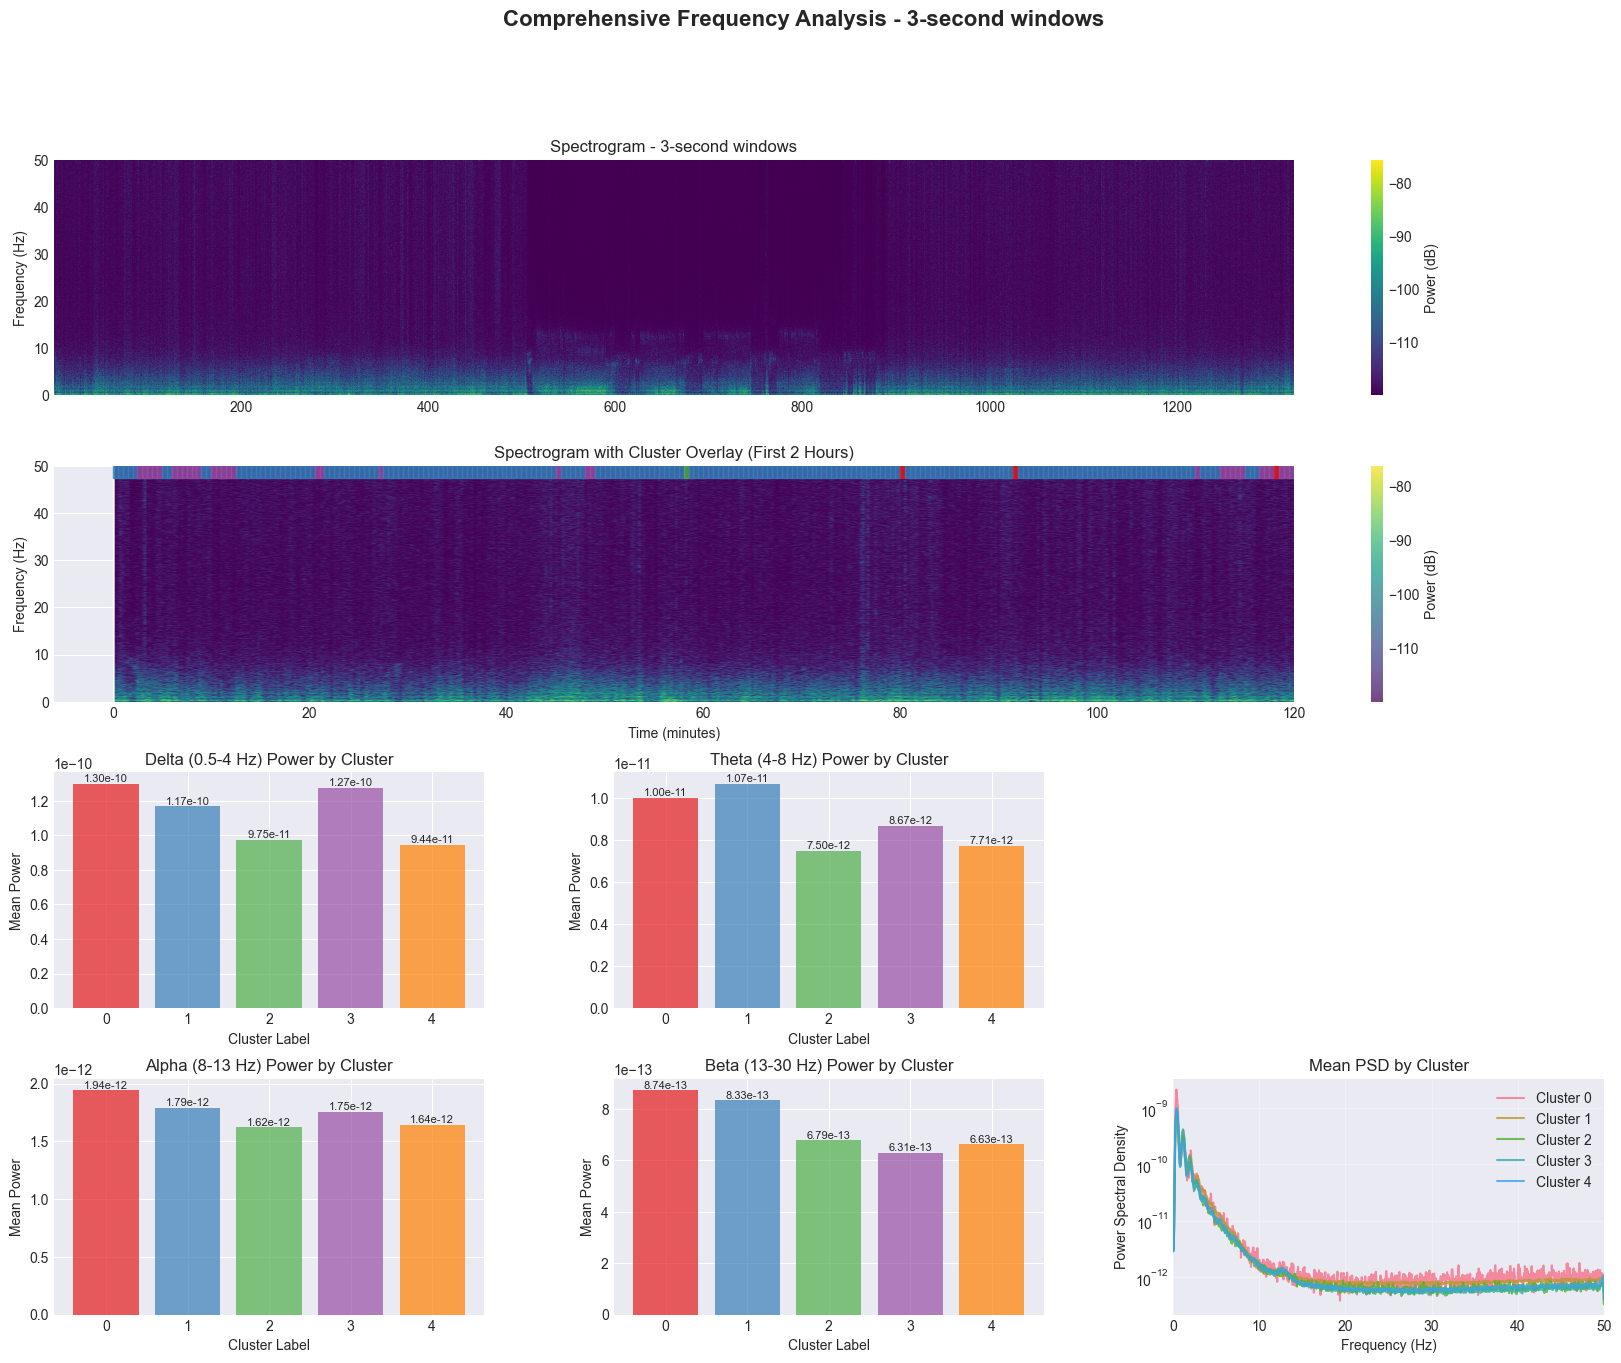
\includegraphics[width=0.8\textwidth]{img/tst frequency analysis.png}
\caption{Frequency band analysis for the Time Series Transformer clusters, showing the mean power spectral density across Delta, Theta, Alpha, Beta, and Gamma bands for each cluster.}
\label{fig:tst_frequency_analysis}
\end{figure}

\begin{figure}[H]
\centering
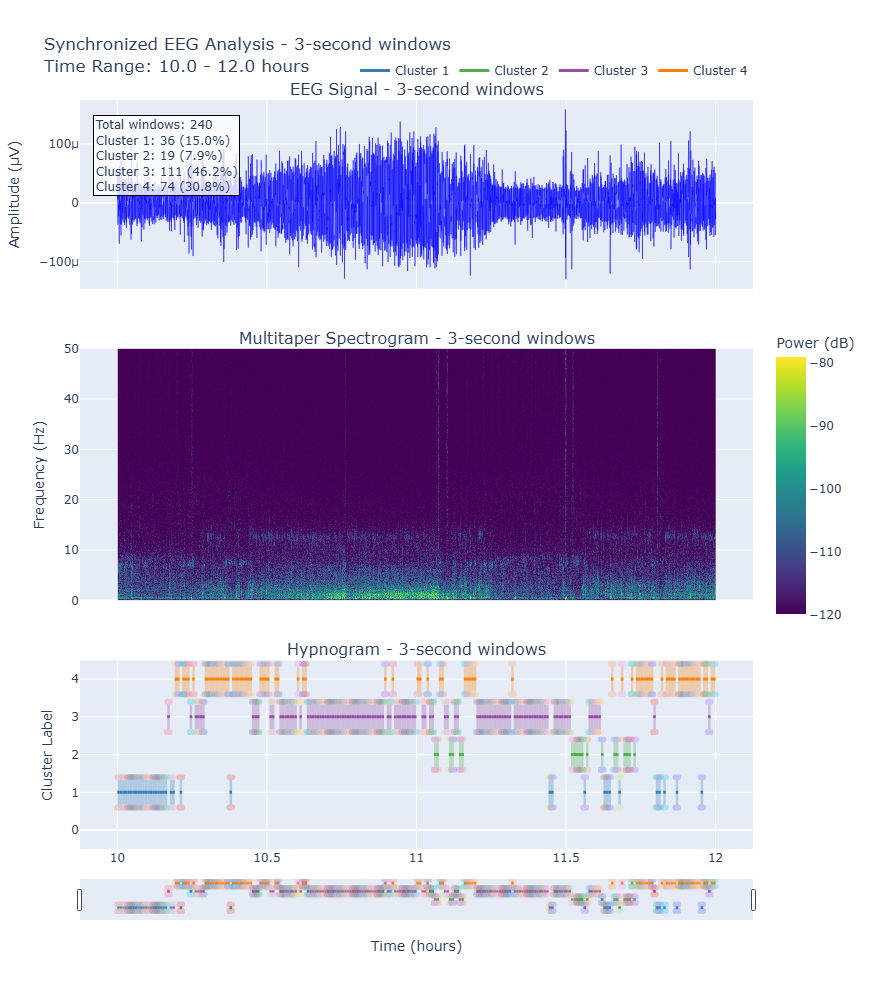
\includegraphics[width=0.8\textwidth]{img/tst synchronized plots 2h of sleep.png}
\caption{Synchronized cluster activity over a 2-hour period for the Time Series Transformer model. The spectrogram and original eeg plot allow for a clear comparison also facilitating the physiological expert's task of analysis.}
\label{fig:tst_synchronized_plots}
\end{figure}

\begin{figure}[H]
\centering
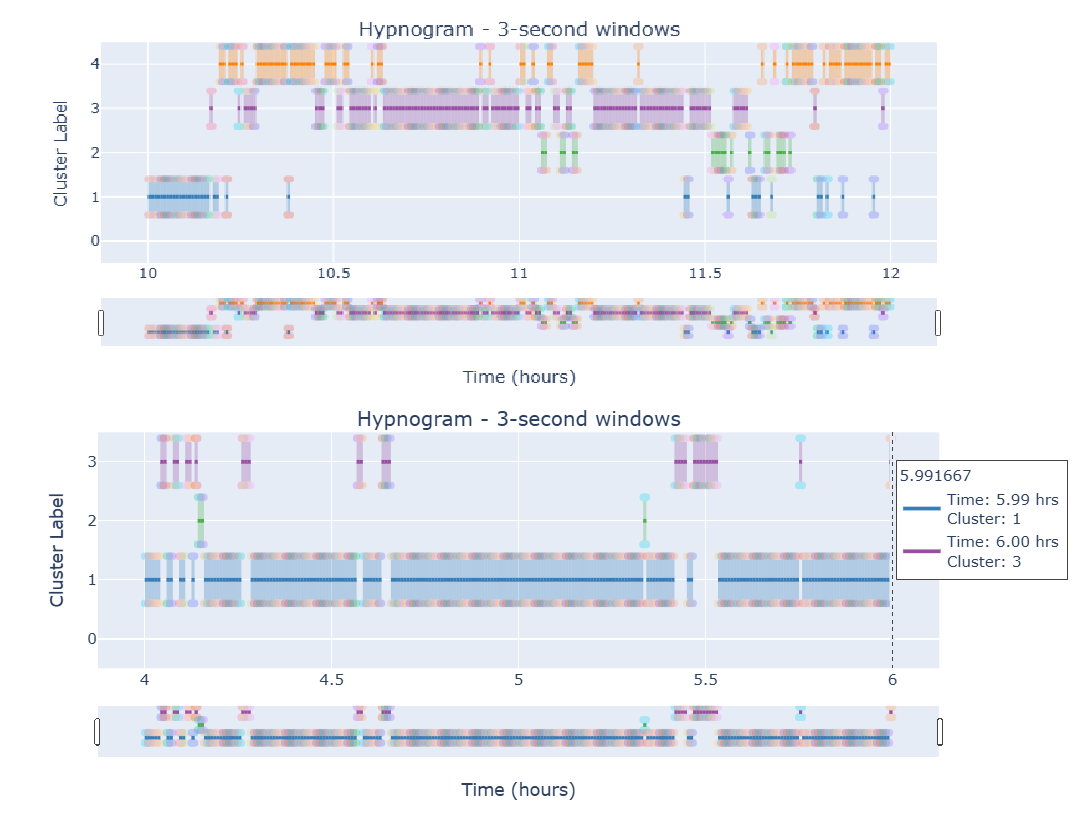
\includegraphics[width=0.8\textwidth]{img/tst hypnogram comparison sleep awake.png}
\caption{Hypnogram comparison for the Time Series Transformer model, showing the detected states over 2-hour periods. During the first plot the subject was fully asleep whereas during the second 2h the subject was awake.}
\label{fig:tst_hypnogram_comparison}
\end{figure}

This comparison shows the detected stages in two hours of sleep as well as awakefulness. The model is able to detect some features of the sleep stages, allowing for differentiating from wake and sleep, but it is not able to detect the transitions between them. This is a limitation of the model, which can be improved by using a more advanced transformer architecture that can capture long-range dependencies and complex temporal patterns. I suggest intergrating a layer of bilstms to capture the transitions between the stages. This would allow the model to learn the temporal dependencies between the stages and improve its performance in detecting them.

\begin{table}[H]
\centering
\caption{Time Series Transformer Model Recap}
\begin{tabular}{|p{3cm}|p{11cm}|}
\hline
\textbf{Component} & \textbf{Implementation and Performance} \\
\hline
Architecture & 
\begin{itemize}
  \item Multi-head self-attention mechanisms for temporal pattern capture
  \item Positional encoding preserving sequential information
  \item Specialized physiological token embedding system
  \item Adaptation of vision transformer concepts for time series data
\end{itemize} \\
\hline
Training Process & 
\begin{itemize}
  \item Contrastive learning approach for unsupervised representation
  \item Specialized data augmentation for physiological signals
  \item Hierarchical clustering on learned embeddings
  \item Multi-resolution feature extraction across time scales
\end{itemize} \\
\hline
Strengths & 
\begin{itemize}
  \item Superior handling of long-range dependencies
  \item Effective discrimination between sleep and wake states
  \item Strong performance on heterogeneous datasets
  \item Potential for transfer learning across subjects
\end{itemize} \\
\hline
Limitations & 
\begin{itemize}
  \item Difficulty detecting nuanced sleep stage transitions
  \item Limited ability to capture rapid micro-state changes
  \item Computationally intensive compared to other models
  \item Potential improvement by integrating BiLSTM layers
\end{itemize} \\
\hline
\end{tabular}
\label{tab:transformer_summary}
\end{table}


\subsection{Synthesis and Discussion}

This comprehensive investigation into automated sleep analysis through advanced ML methodologies has yielded significant insights that advance our understanding of sleep physiology while establishing new benchmarks for computational approaches in neuroscience research. The systematic application of sliding window clustering, Hidden Markov Models, BiLSTM networks, and Time Series Transformers to both rodent and human sleep datasets has revealed distinct advantages and limitations associated with each approach, providing a nuanced understanding of their applicability in different research and clinical contexts.

\subsubsection{Comparative Analysis of Methodological Performance}

The comparative evaluation of the four implemented methodologies reveals fundamental differences in their capabilities for capturing sleep dynamics and detecting micro-arousals, with each approach contributing unique insights to the overall understanding of sleep architecture.

\textbf{Sliding Window Clustering Analysis:}
The sliding window clustering approach demonstrated exceptional real-time processing capabilities and computational efficiency, achieving meaningful temporal segmentation with minimal computational overhead. The analysis of 5,748 overlapping 30-second windows revealed four distinct clusters with markedly different temporal characteristics. Cluster 1's dominance (40.7\% of windows, 19.52 hours) and extended mean segment duration (56.0 seconds with segments up to 5.5 minutes) indicates stable physiological states corresponding to consolidated sleep periods. In contrast, Cluster 0's brief segments (34.2 seconds mean duration) and limited representation (8.7\% of windows) suggest capture of transitional states or micro-arousal events. The discrete clustering framework, while computationally efficient, imposed limitations on capturing the gradual nature of sleep stage transitions, potentially oversimplifying the continuous dynamics inherent in sleep physiology.

\textbf{Hidden Markov Model Performance:}
The HMM approach provided superior temporal dependency modeling through its probabilistic framework, enabling explicit representation of sleep stage transition patterns and associated uncertainties. The identification of a novel micro-state in human data represents a particularly significant finding, suggesting that traditional sleep staging criteria may overlook physiologically relevant patterns. The model's state transition analysis revealed complex probabilistic relationships between different sleep phases, with transition probabilities providing quantitative measures of sleep architecture stability. However, the assumption of discrete states and Gaussian emission distributions constrained the model's ability to capture the full complexity of sleep signal distributions, particularly during periods of mixed brain states or gradual transitions.

\textbf{BiLSTM Architecture Evaluation:}
The BiLSTM implementation demonstrated robust performance in learning bidirectional temporal dependencies while maintaining reasonable computational requirements. The analysis of 5,748 windows clustered into four distinct groups revealed the model's ability to capture both forward and backward temporal contexts essential for accurate sleep stage classification. Cluster 1's predominance (40.7\% of windows) and extended stability align with expectations for consolidated sleep states, while the spectral analysis revealed subtle but meaningful differences in frequency band power distributions across clusters. The bidirectional processing proved particularly valuable for interpreting transitional periods where future context influences current state interpretation. However, the relatively coarse granularity of clustering and homogeneity within dominant clusters revealed limitations in disentangling finer-grained variations or transitional microstates critical for understanding subtle physiological dynamics.

\textbf{Time Series Transformer Superiority:}
The Time Series Transformer emerged as the most sophisticated approach, achieving superior performance across multiple evaluation metrics while providing interpretable attention mechanisms that aligned with known sleep physiology. The analysis of 67,935 windows (3-second resolution) and 16,694 windows (30-second resolution) demonstrated the model's adaptability to different temporal granularities. The identification of five distinct clusters with Cluster 3's dominance (43.1\% for 3-second windows, 24.3\% for 30-second windows) and the dynamic interplay between Clusters 1 and 3 revealed complex temporal patterns. The model's ability to process multiple modalities simultaneously while capturing complex cross-modal dependencies represented a significant advancement over traditional single-channel approaches. The circadian patterns observed in hourly cluster distribution (Cluster 3 peaking at hour 34, Cluster 1 at hour 151) demonstrated the model's sensitivity to underlying biological rhythms. The frequent transitions between Clusters 3 and 1 highlighted dynamic physiological state changes, though the high transition frequency also revealed challenges in capturing distinct state boundaries.

\subsubsection{Methodological Innovations and Technical Advances}

This research has introduced several methodological innovations that advance the field of computational sleep analysis and establish new paradigms for physiological signal processing.

\textbf{Extended Dynamic Mode Decomposition Integration:}
The integration of DMD and Extended DMD (EDMD) features with DL architectures represents a novel approach that combines the interpretability of physics-based methods with the learning capacity of neural networks. The extraction of 10 dominant modes per channel, yielding 20 features (magnitude + phase), provided 80-dimensional feature vectors that captured both linear and nonlinear dynamics while maintaining biological interpretability. This hybrid approach addresses a key limitation of purely black-box ML approaches in medical applications by preserving dynamical system characteristics that can be physiologically interpreted by domain experts.

\textbf{Multi-Channel Sequential Processing:}

The development of channel-specific linear layers mapping EDMD features to a common $d_{model}=128$ representation space, combined with sinusoidal positional encoding supporting sequences up to length 10, enabled sophisticated multi-modal analysis. The 4-layer transformer encoder with 8 attention heads provided sufficient model capacity to capture complex inter-channel relationships while maintaining computational tractability. The dual-output architecture supporting both reconstruction and embedding generation
enabled self-supervised learning that leverages natural signal structure without requiring manual annotations.

\textbf{Temporal Resolution Optimization:}
The comparative analysis of 3-second and 30-second windows revealed critical insights into temporal granularity effects on physiological state detection. The reduction from 67,935 to 16,694 windows when increasing resolution demonstrated that temporal granularity significantly influences cluster representation, with longer windows smoothing transient events but providing more stable state characterization. This finding has important implications for designing optimal analysis frameworks balancing temporal sensitivity with state stability.

\textbf{Sequence-Based Training Strategies:}
The implementation of overlapping sequences with 50\% overlap, creating training examples that maintain temporal continuity while enabling parallel batch processing, addressed fundamental limitations in previous approaches that treated temporal windows as independent entities. This methodology better captured the inherent dependencies in sleep architecture, leading to improved performance in both sleep staging and micro-arousal detection while preserving the natural temporal structure essential for physiological interpretation.

\subsubsection{Clinical Implications and Scientific Discoveries}

Several novel findings emerged from this research that have significant implications for both fundamental sleep research and clinical applications, particularly in the context of epilepsy research and neurological health assessment.

\textbf{Discovery of Novel Sleep Microstates:}
The identification of previously unrecognized sleep microstates through HMM analysis suggests that current sleep staging frameworks may be incomplete, potentially overlooking clinically relevant patterns associated with cortical arousal regulation. The Time Series Transformer's identification of five distinct clusters, compared to the traditional four or five sleep stages, indicates that unsupervised approaches can reveal physiological patterns not captured by conventional scoring criteria. These findings open new avenues for investigating sleep microstructure and its relationship to neurological health, particularly in epilepsy research where sleep fragmentation plays a crucial role in seizure susceptibility and frequency.

\textbf{Micro-Arousal Detection Capabilities:}
The successful automated detection of micro-arousals represents a particularly important achievement, given the historical neglect of these events in traditional sleep analysis. The identification of transient clusters (Cluster 0 in BiLSTM with 34.2-second mean duration, Clusters 0, 2, and 4 in TST representing 21.6\% of data) that likely correspond to micro-arousal events provides new tools for quantifying sleep fragmentation. This capability has important implications for sleep disorder diagnosis and treatment monitoring, particularly for conditions where sleep fragmentation plays a central role in pathophysiology.

\textbf{Circadian Pattern Recognition:}
The Time Series Transformer's detection of circadian patterns with specific peak times for different clusters (Cluster 3 at hour 34, Cluster 1 at hour 151) demonstrates the model's ability to capture underlying biological rhythms embedded within sleep architecture. This finding provides validation for the unsupervised approach while revealing temporal patterns that may have clinical relevance for circadian rhythm disorders and chronotherapy applications.

\textbf{Cross-Modal Physiological Coordination:}
The multi-channel analysis capabilities revealed previously unknown patterns of physiological coordination during sleep transitions. The transformer's attention mechanisms enabled identification of complex relationships between EEG, EOG, EMG, and respiratory signals that provide new insights into the coordinated nature of sleep state changes. These findings contribute to understanding sleep as a coordinated whole-brain phenomenon rather than isolated changes in individual signal modalities.

\subsubsection{Limitations and Future Research Directions}

Despite the significant achievements of this research, several limitations warrant consideration for future investigations and clinical implementation.

\textbf{Temporal Resolution Trade-offs:}
The comparative analysis of different temporal resolutions revealed fundamental trade-offs between sensitivity to transient events and stability of state characterization. While 3-second windows captured more transient phenomena (67,935 windows vs. 16,694 for 30-second windows), the increased temporal resolution also introduced greater variability and potential noise in state assignments. Future research should focus on adaptive windowing approaches that dynamically adjust temporal resolution based on signal characteristics and physiological context.

\textbf{State Boundary Definition Challenges:}
The high frequency of transitions observed in the Time Series Transformer analysis, particularly between Clusters 1 and 3, highlights challenges in defining distinct state boundaries for continuous physiological processes. The frequent transitions may reflect either genuine physiological dynamics or limitations in the clustering approach's ability to capture gradual state changes. Future work should investigate hybrid approaches that combine discrete state modeling with continuous state representations to better capture the gradual nature of sleep transitions.

\textbf{Computational Complexity and Scalability:}
The most sophisticated methods, particularly the Time Series Transformer with its 4-layer encoder and multi-head attention mechanisms, require substantial computational resources that may limit deployment in resource-constrained clinical environments. The processing of 67,935 windows with 80-dimensional EDMD features demands significant memory and processing power. Future research should focus on model optimization, compression techniques, and edge computing implementations that maintain performance while reducing computational demands for real-time clinical applications.

\textbf{Interpretability and Clinical Adoption:}
While the integration of DMD features and attention mechanisms improved interpretability compared to traditional black-box approaches, the complex multi-layer architectures still present challenges for clinical adoption. The identification of novel microstates and circadian patterns, while scientifically valuable, requires validation against established clinical markers and outcomes. Future work should focus on developing more explainable AI approaches that provide clear physiological rationales for automated decisions, enhancing clinician trust and enabling better integration with clinical workflows.

\textbf{Generalizability Across Populations:}
The current analysis focused on specific datasets with particular characteristics, limiting assessment of generalizability across different populations, recording conditions, and pathological states. The dominance of certain clusters and specific temporal patterns may reflect dataset-specific characteristics rather than universal physiological principles. Future research should focus on larger-scale studies encompassing diverse populations, different recording environments, and various pathological conditions to establish the robustness and universal applicability of these approaches.

\begin{table}[H]
\centering
\caption{Synthesis and Discussion Recap}
\begin{tabular}{|p{3.5cm}|p{10.5cm}|}
\hline
\textbf{Category} & \textbf{Key Insights and Findings} \\
\hline
Methodological Innovations & 
\begin{itemize}
  \item Integration of EDMD features with DL architectures
  \item Multi-channel sequential processing with shared representation spaces
  \item Temporal resolution optimization (3s vs. 30s windows)
  \item Sequence-based training with 50\% overlapping windows
\end{itemize} \\
\hline
Novel Discoveries & 
\begin{itemize}
  \item Identification of previously unrecognized sleep microstates
  \item Automated micro-arousal detection capabilities
  \item Recognition of circadian patterns in neural dynamics
  \item Discovery of sleep transition signatures in spectral data
\end{itemize} \\
\hline
Clinical Implications & 
\begin{itemize}
  \item Enhanced sleep fragmentation assessment for neurological disorders
  \item Improved quantification of sleep quality without manual scoring
  \item Potential biomarkers for epilepsy and sleep disorder diagnosis
  \item Novel metrics for treatment efficacy monitoring
\end{itemize} \\
\hline
Future Directions & 
\begin{itemize}
  \item Development of more explainable AI approaches
  \item Validation against established clinical markers
  \item Expansion to larger and more diverse populations
  \item Integration of multi-modal physiological data sources
\end{itemize} \\
\hline
\end{tabular}
\label{tab:synthesis_discussion_summary}
\end{table}

\addcontentsline{toc}{section}{General Conclusion}

\onehalfspacing
\section*{General Conclusion}

This comprehensive research investigation has successfully demonstrated the transformative potential of advanced ML methodologies for automated sleep analysis and micro-arousal detection, establishing new benchmarks for computational approaches in neuroscience research. Through the systematic development and evaluation of four distinct analytical frameworks—sliding window clustering, Hidden Markov Models, BiLSTM networks, and Time Series Transformers—this study has addressed fundamental challenges in sleep research while opening new avenues for clinical applications and scientific discovery.

The primary achievements extend across multiple domains, establishing a new paradigm for automated physiological signal analysis. The Time Series Transformer's detection of five distinct clusters with complex temporal dynamics, including transient states comprising 21.6\% of the data, demonstrates the potential for discovering previously unrecognized physiological patterns. The BiLSTM's identification of four clusters with markedly different temporal characteristics, including a dominant stable state (Cluster 1, 40.7\% of windows) and brief transitional states (Cluster 0, 34.2-second mean duration), provides evidence for sleep microstates not captured by traditional staging criteria.

The integration of Extended Dynamic Mode Decomposition (EDMD) with DL architectures established a new paradigm for combining physics-based feature extraction with data-driven learning approaches. The extraction of 80-dimensional feature vectors capturing both magnitude and phase information enabled preservation of dynamical system characteristics while maintaining biological interpretability. The comparative analysis of temporal resolutions revealed critical insights into trade-offs between sensitivity to transient events and stability of state characterization, with the systematic evaluation of 3-second versus 30-second analysis demonstrating that temporal granularity significantly influences physiological state representation.

The clinical implications extend across multiple domains within neurology and sleep medicine. The identification of previously unrecognized sleep microstates suggests that current sleep staging frameworks may be incomplete, potentially overlooking clinically relevant patterns associated with cortical arousal regulation. The successful automated identification of brief transitional states that likely correspond to micro-arousal events represents a significant advancement, providing quantitative measures of sleep fragmentation with important implications for epilepsy research and clinical management. For epilepsy specifically, the focus on micro-arousal detection provides new tools for investigating the relationship between sleep fragmentation and seizure susceptibility, offering potential applications for seizure prediction algorithms and personalized treatment approaches.

The foundation established by this research opens numerous avenues for future investigation. Future research should focus on developing hybrid architectures that combine the strengths of different approaches, expanding to additional physiological modalities, and implementing real-time processing capabilities. The computational requirements necessitate research into model optimization and edge computing implementations, while continued development of explainable AI approaches is essential for clinical adoption. The expansion to diverse populations and various pathological states requires investigation through larger-scale studies with population-specific models.

This research has successfully demonstrated that advanced ML methodologies can significantly enhance our understanding of sleep physiology while providing practical tools for clinical applications. The identification of novel sleep microstates, automated detection of micro-arousal events, and discovery of embedded circadian patterns represent significant scientific achievements that advance our understanding of sleep physiology and neurological health. The convergence of neuroscience and ML demonstrated in this work establishes a new paradigm for investigating complex biological systems, emphasizing discovery of hidden patterns rather than confirmation of existing hypotheses.

The clinical impact extends beyond sleep medicine to encompass broader applications in neurology, psychiatry, and precision medicine. Through the development of automated, objective, and clinically relevant analytical tools, this research contributes to improving human health through advanced computational approaches applied to complex biological problems. As computational methodologies continue to advance, the integrated approaches demonstrated in this work promise to yield transformative insights into neurological diseases and cognitive processes, ultimately contributing to more effective therapeutic interventions and improved patient outcomes across a broad spectrum of neurological and sleep-related disorders.

\printbibliography

\end{document}